% Options for packages loaded elsewhere
\PassOptionsToPackage{unicode}{hyperref}
\PassOptionsToPackage{hyphens}{url}
%
\documentclass[
]{book}
\usepackage{amsmath,amssymb}
\usepackage{lmodern}
\usepackage{iftex}
\ifPDFTeX
  \usepackage[T1]{fontenc}
  \usepackage[utf8]{inputenc}
  \usepackage{textcomp} % provide euro and other symbols
\else % if luatex or xetex
  \usepackage{unicode-math}
  \defaultfontfeatures{Scale=MatchLowercase}
  \defaultfontfeatures[\rmfamily]{Ligatures=TeX,Scale=1}
\fi
% Use upquote if available, for straight quotes in verbatim environments
\IfFileExists{upquote.sty}{\usepackage{upquote}}{}
\IfFileExists{microtype.sty}{% use microtype if available
  \usepackage[]{microtype}
  \UseMicrotypeSet[protrusion]{basicmath} % disable protrusion for tt fonts
}{}
\makeatletter
\@ifundefined{KOMAClassName}{% if non-KOMA class
  \IfFileExists{parskip.sty}{%
    \usepackage{parskip}
  }{% else
    \setlength{\parindent}{0pt}
    \setlength{\parskip}{6pt plus 2pt minus 1pt}}
}{% if KOMA class
  \KOMAoptions{parskip=half}}
\makeatother
\usepackage{xcolor}
\usepackage{color}
\usepackage{fancyvrb}
\newcommand{\VerbBar}{|}
\newcommand{\VERB}{\Verb[commandchars=\\\{\}]}
\DefineVerbatimEnvironment{Highlighting}{Verbatim}{commandchars=\\\{\}}
% Add ',fontsize=\small' for more characters per line
\usepackage{framed}
\definecolor{shadecolor}{RGB}{248,248,248}
\newenvironment{Shaded}{\begin{snugshade}}{\end{snugshade}}
\newcommand{\AlertTok}[1]{\textcolor[rgb]{0.94,0.16,0.16}{#1}}
\newcommand{\AnnotationTok}[1]{\textcolor[rgb]{0.56,0.35,0.01}{\textbf{\textit{#1}}}}
\newcommand{\AttributeTok}[1]{\textcolor[rgb]{0.77,0.63,0.00}{#1}}
\newcommand{\BaseNTok}[1]{\textcolor[rgb]{0.00,0.00,0.81}{#1}}
\newcommand{\BuiltInTok}[1]{#1}
\newcommand{\CharTok}[1]{\textcolor[rgb]{0.31,0.60,0.02}{#1}}
\newcommand{\CommentTok}[1]{\textcolor[rgb]{0.56,0.35,0.01}{\textit{#1}}}
\newcommand{\CommentVarTok}[1]{\textcolor[rgb]{0.56,0.35,0.01}{\textbf{\textit{#1}}}}
\newcommand{\ConstantTok}[1]{\textcolor[rgb]{0.00,0.00,0.00}{#1}}
\newcommand{\ControlFlowTok}[1]{\textcolor[rgb]{0.13,0.29,0.53}{\textbf{#1}}}
\newcommand{\DataTypeTok}[1]{\textcolor[rgb]{0.13,0.29,0.53}{#1}}
\newcommand{\DecValTok}[1]{\textcolor[rgb]{0.00,0.00,0.81}{#1}}
\newcommand{\DocumentationTok}[1]{\textcolor[rgb]{0.56,0.35,0.01}{\textbf{\textit{#1}}}}
\newcommand{\ErrorTok}[1]{\textcolor[rgb]{0.64,0.00,0.00}{\textbf{#1}}}
\newcommand{\ExtensionTok}[1]{#1}
\newcommand{\FloatTok}[1]{\textcolor[rgb]{0.00,0.00,0.81}{#1}}
\newcommand{\FunctionTok}[1]{\textcolor[rgb]{0.00,0.00,0.00}{#1}}
\newcommand{\ImportTok}[1]{#1}
\newcommand{\InformationTok}[1]{\textcolor[rgb]{0.56,0.35,0.01}{\textbf{\textit{#1}}}}
\newcommand{\KeywordTok}[1]{\textcolor[rgb]{0.13,0.29,0.53}{\textbf{#1}}}
\newcommand{\NormalTok}[1]{#1}
\newcommand{\OperatorTok}[1]{\textcolor[rgb]{0.81,0.36,0.00}{\textbf{#1}}}
\newcommand{\OtherTok}[1]{\textcolor[rgb]{0.56,0.35,0.01}{#1}}
\newcommand{\PreprocessorTok}[1]{\textcolor[rgb]{0.56,0.35,0.01}{\textit{#1}}}
\newcommand{\RegionMarkerTok}[1]{#1}
\newcommand{\SpecialCharTok}[1]{\textcolor[rgb]{0.00,0.00,0.00}{#1}}
\newcommand{\SpecialStringTok}[1]{\textcolor[rgb]{0.31,0.60,0.02}{#1}}
\newcommand{\StringTok}[1]{\textcolor[rgb]{0.31,0.60,0.02}{#1}}
\newcommand{\VariableTok}[1]{\textcolor[rgb]{0.00,0.00,0.00}{#1}}
\newcommand{\VerbatimStringTok}[1]{\textcolor[rgb]{0.31,0.60,0.02}{#1}}
\newcommand{\WarningTok}[1]{\textcolor[rgb]{0.56,0.35,0.01}{\textbf{\textit{#1}}}}
\usepackage{longtable,booktabs,array}
\usepackage{calc} % for calculating minipage widths
% Correct order of tables after \paragraph or \subparagraph
\usepackage{etoolbox}
\makeatletter
\patchcmd\longtable{\par}{\if@noskipsec\mbox{}\fi\par}{}{}
\makeatother
% Allow footnotes in longtable head/foot
\IfFileExists{footnotehyper.sty}{\usepackage{footnotehyper}}{\usepackage{footnote}}
\makesavenoteenv{longtable}
\usepackage{graphicx}
\makeatletter
\def\maxwidth{\ifdim\Gin@nat@width>\linewidth\linewidth\else\Gin@nat@width\fi}
\def\maxheight{\ifdim\Gin@nat@height>\textheight\textheight\else\Gin@nat@height\fi}
\makeatother
% Scale images if necessary, so that they will not overflow the page
% margins by default, and it is still possible to overwrite the defaults
% using explicit options in \includegraphics[width, height, ...]{}
\setkeys{Gin}{width=\maxwidth,height=\maxheight,keepaspectratio}
% Set default figure placement to htbp
\makeatletter
\def\fps@figure{htbp}
\makeatother
\setlength{\emergencystretch}{3em} % prevent overfull lines
\providecommand{\tightlist}{%
  \setlength{\itemsep}{0pt}\setlength{\parskip}{0pt}}
\setcounter{secnumdepth}{5}
\usepackage{booktabs}
\ifLuaTeX
  \usepackage{selnolig}  % disable illegal ligatures
\fi
\usepackage[]{natbib}
\bibliographystyle{plainnat}
\IfFileExists{bookmark.sty}{\usepackage{bookmark}}{\usepackage{hyperref}}
\IfFileExists{xurl.sty}{\usepackage{xurl}}{} % add URL line breaks if available
\urlstyle{same} % disable monospaced font for URLs
\hypersetup{
  pdftitle={Introdução à linguagem R},
  pdfauthor={Jean S. S. Resende, Jéssica M. Magno, João C. D. Muzzi, Mauro A. A. Castro},
  hidelinks,
  pdfcreator={LaTeX via pandoc}}

\title{Introdução à linguagem R}
\author{Jean S. S. Resende, Jéssica M. Magno, João C. D. Muzzi, Mauro A. A. Castro}
\date{2023-06-06}

\begin{document}
\maketitle

{
\setcounter{tocdepth}{1}
\tableofcontents
}
\hypertarget{prefuxe1cio}{%
\chapter{Prefácio}\label{prefuxe1cio}}

A linguagem R foi criada por professores do departamento de estatística da univer sidade de Auckland no ano 2000. A intenção destes professores era disponibilizar uma linguagem \emph{open-source} para computação estatística. Com o avanço e popularização da linguagem, profissionais de diversas áreas passaram a utilizá-la em suas análises de dados.

Esta apostila contém uma introdução à linguagem de programação R. Aborda desde conteúdos teóricos quanto práticos, com exemplos didáticos a fim de facilitar o aprendizado. Esta apostila foi produzida principalmente pelos autores: Jean Silva de Souza Resende, Jéssica Maria Magno, João Carlos Degram Muzzi sob orientação de Mauro Antônio Alves Castro. Em versões anteriores, tivemos a colaboração dos autores: Sheyla Trefflich, Danrley R. Fernandes e Giuseppe Pasqualato Neto.

\hypertarget{introduuxe7uxe3o}{%
\chapter{Introdução}\label{introduuxe7uxe3o}}

\hypertarget{contextualizando-a-linguagem-de-programauxe7uxe3o-r}{%
\section{Contextualizando a linguagem de programação R}\label{contextualizando-a-linguagem-de-programauxe7uxe3o-r}}

A linguagem R é uma linguagem de programação com o foco em computação estatística e manipulação de gráficos. Criada no início dos anos 90 por \href{https://en.wikipedia.org/wiki/Ross_Ihaka}{Geroge Ross Ihaka} e \href{https://en.wikipedia.org/wiki/Robert_Gentleman_(statistician)}{Robert Clifford Gentleman}, o R é usado mais utilizado por estatísticos, bioinformatas, analistas de dados e desenvolvedor de \emph{software} estatístico. No entanto ele tem se destacado na comunidade científica. Em maio de 2023, o R ocupava a 16ª posição no \href{https://www.tiobe.com/tiobe-index/}{índice TIOBE}, uma medida de popularidade da linguagem de programação, sendo que em agosto de 2020 o R atingiu seu pico em ficando 8º lugar.

O R é um ambiente de \emph{software} livre de código aberto, disponível sob a \href{https://en.wikipedia.org/wiki/GNU_General_Public_License}{\emph{GNU General Public License}}. Seus executáveis pré-compilados são fornecidos para vários sistemas operacionais. Ele tem uma interface de linha de comando, mas também possui interfaces gráficas de usuário (GUI) de terceiros como o \href{https://posit.co/download/rstudio-desktop/}{Rstudio} - que será a IDE (\emph{Integrated Development Envirenment}) que iremos utilizar na apostila.

\hypertarget{instalauxe7uxe3o-do-r}{%
\section{Instalação do R}\label{instalauxe7uxe3o-do-r}}

\begin{enumerate}
\def\labelenumi{\arabic{enumi}.}
\tightlist
\item
  Acesse o repositório do R (\href{https://cran-r.c3sl.ufpr.br/}{clique aqui}).
\item
  Acesse o link referente ao seu sitema operacional: Linux, macOS ou Windows.
  2.1. Linux: escolha a distribuição linux (debian, fedora, redhat, suse ou ubuntu) e então prossiga com os comandos no terminal.
  2.2. macOS: escolha o instalador conforme o modelo da sua máquina e execute-o.
  2.3. Windows: acesse o link Base e então baixe o instalador e execute-o.
\end{enumerate}

\hypertarget{instalauxe7uxe3o-do-rstudio}{%
\section{Instalação do RStudio}\label{instalauxe7uxe3o-do-rstudio}}

\begin{enumerate}
\def\labelenumi{\arabic{enumi}.}
\tightlist
\item
  \href{https://posit.co/download/rstudio-desktop/}{Clique aqui} para acessar o repositório do RStudio.
\item
  Baixe o instalador conforme o sistema operacional da sua máquina (Linux/macOS/Windows).
\end{enumerate}

\hypertarget{interface-do-rstudio}{%
\section{Interface do RStudio}\label{interface-do-rstudio}}

Por padrão o RStudio abre quatro janelas (pode ocorrer de uma estar oculta, mas observe o botão de minimizar/maximizar no canto superior direito de cada janela).

\begin{itemize}
\tightlist
\item
  \textbf{Editor de código} (\emph{janela do canto superior esquerdo}): Nela você digita os comando a serem executados no RStudio. Para executá-los aperte as teclas `CTRL' e `ENTER' simultaneamente na linha ou bloco de código selecionado.
\item
  \textbf{Console} (\emph{janela do canto inferior esquerdo}): É visto as saídas dos comandos que são rodados. Também é possível digitar e rodar códigos diretamente nesta janela.
\item
  \textbf{Histórico} (\emph{janela do canto superior direito}): Nesta janela ficam salvos os objetos, históricos de comandos e conexões com outros aplicativos.
\item
  \textbf{Visualização} (\emph{janela do canto inferior direito}): Aqui você pode visualizar os gráficos no RStudio, navegar entre os arquivos do seu computador, visualizar os pacotes instalados e ver a ajuda de comandos e descrições de tabelas de dados e por fim navegar entre os arquivos html.
\end{itemize}

\begin{figure}
\centering
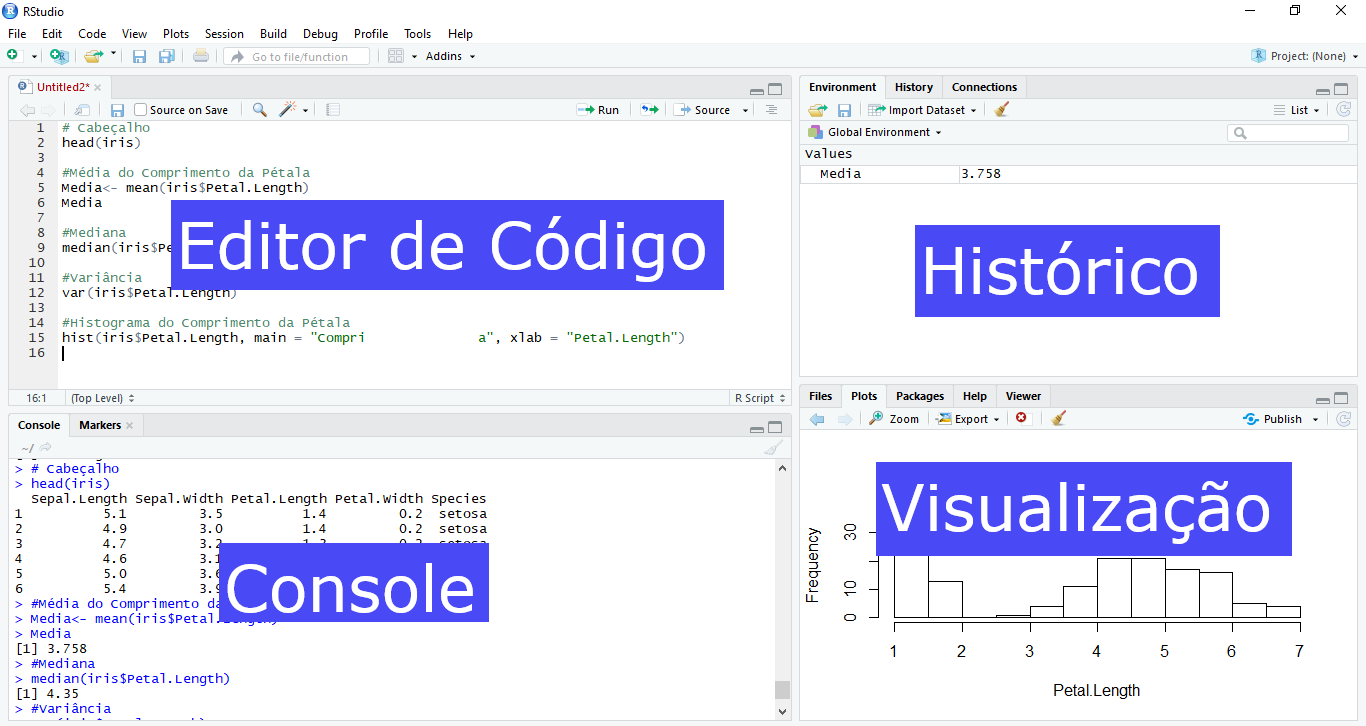
\includegraphics{figure/fig1_rstudio.png}
\caption{Janelas do RStudio. Ref: \url{https://www.est.ufmg.br/~cristianocs/Pacotes2021/Intro.html\#6}}
\end{figure}

\hypertarget{pacotes}{%
\section{Pacotes}\label{pacotes}}

Por ser \emph{Open Source}, o R permite que qualquer usuário disponibilize funções e bancos de dados a comunidade. As funções/bancos de dados são disponibilizados através de pacotes. A instalação de um pacote depende do repositório que ele está armazenado: máquina local, CRAN, GitHub, Bioconductor, entre outros. O repostitório CRAN contêm muitos pacotes e não é direcionado à uma área específica (como é o caso do Bioconductor que se destina a pacotes voltados para área de biotecnologia). A instalação de um pacote do repositório CRAN é feita pelo menu ``Tools \textgreater{} Install Packages'' ou simplesmente utilizando o seguinte comando:

\begin{Shaded}
\begin{Highlighting}[]
\FunctionTok{installed.packages}\NormalTok{(}\StringTok{"nomeDoPacote"}\NormalTok{)}
\end{Highlighting}
\end{Shaded}

Para que você possa utilizar as funções do pacote que instalou, você deve usar um dos dois comandos a seguir, para de fato carregar as funções do pacote para o ambiente R:

\begin{Shaded}
\begin{Highlighting}[]
\FunctionTok{library}\NormalTok{(nomeDoPacote)}
\FunctionTok{require}\NormalTok{(nomeDoPacote)}
\end{Highlighting}
\end{Shaded}

A função \texttt{library()} é utilizada normalmente no corpo do script, enquanto que a função \texttt{require()} é utilizada dentro de outras funções.

\hypertarget{comeuxe7ando-de-fato-a-programar-em-r}{%
\section{Começando de fato a programar em R}\label{comeuxe7ando-de-fato-a-programar-em-r}}

No console (janela do canto inferior esquerdo) digite o comando a seguir e tecle ENTER:

\begin{Shaded}
\begin{Highlighting}[]
\FunctionTok{print}\NormalTok{(}\StringTok{"Hello World"}\NormalTok{)}
\end{Highlighting}
\end{Shaded}

Agora digite o mesmo comando no editor de código (janela do canto superior esquerdo) e com o cursor na mesma linha do comando, tecle CTRL e ENTER simultaneamente:

\begin{Shaded}
\begin{Highlighting}[]
\FunctionTok{print}\NormalTok{(}\StringTok{"Hello World"}\NormalTok{)}
\end{Highlighting}
\end{Shaded}

A diferença é que quando executamos os comandos no editor de código, o comando continua no editor para ser executado, ou seja svocê está construindo um script. Mas você executa comando diretamente no console, eles não ficam gravados em um editor.

O dado de saída da função, foi um print do que estava dentro da função. Mas como você saber o que usar dentro de uma determinada função, como \texttt{print()}? Você precisa acessar o manual desta função.

\hypertarget{acessando-o-manual-da-funuxe7uxe3o}{%
\section{Acessando o manual da função}\label{acessando-o-manual-da-funuxe7uxe3o}}

Esta é uma etapa muito importante que antecede a sua caminhada no aprendizado do R. Você pode visualizar o manual da função executando um comando onde um ponto de interregoção (?) precisa anteceder a função:

\begin{Shaded}
\begin{Highlighting}[]
\NormalTok{?print}
\end{Highlighting}
\end{Shaded}

Mas se você deseja encontrar funções que realizam uma determinada ação, basta inserir dois pontos de interrogação antecedendo a ação desejada:

\begin{Shaded}
\begin{Highlighting}[]
\NormalTok{??priting}
\end{Highlighting}
\end{Shaded}

O comando acima realizará uma busca por tópicos que contenham a palavra \emph{ploting}. Outra opçõe alternativa ao \textbf{?} é o uso da função \texttt{help()} e \texttt{help.search()} para \textbf{??}

\begin{Shaded}
\begin{Highlighting}[]
\FunctionTok{help}\NormalTok{(}\StringTok{"print"}\NormalTok{)}
\FunctionTok{help.search}\NormalTok{(}\StringTok{"priting"}\NormalTok{)}
\end{Highlighting}
\end{Shaded}

Algumas funções possuem exemplos de sua execução. Se você quer saber como utilizar uma determinada função através de exemplos, execute a função \texttt{example()}.

\begin{Shaded}
\begin{Highlighting}[]
\FunctionTok{example}\NormalTok{(}\StringTok{"print"}\NormalTok{)}
\end{Highlighting}
\end{Shaded}

\hypertarget{comentando-cuxf3digos-no-r}{%
\section{Comentando códigos no R}\label{comentando-cuxf3digos-no-r}}

A maioria das linguagens de programação e até linguagem de marcação, possuem uma forma de inserção de textos que não serão executados pela linguagem. Esse procedimento é denominado de comentário. Você pode comentar os seus códigos. Isso é algo essencial para todos os programadores, indiferente da linguagem. Pois, códigos comentados facilitam a interpretação do mesmo por outros programadores e até mesmo pelo autor, devido a um período de tempo que se passou desde a criação daquele código.

Para comentar linhas no R você precisa inserir o \texttt{\#} antes do que seria o comentário:

\begin{Shaded}
\begin{Highlighting}[]
\CommentTok{\# isto é um comentário}
\end{Highlighting}
\end{Shaded}

Exemplo aplicado:

\begin{Shaded}
\begin{Highlighting}[]
\FunctionTok{print}\NormalTok{(}\StringTok{"Hello World"}\NormalTok{) }\CommentTok{\# imprimindo na tela Hello World}
\end{Highlighting}
\end{Shaded}

Perceba que o conteúdo após o \texttt{\#} não é interpretado no R, ou seja, este conteúdo é um comentário.

\hypertarget{fundamentos-buxe1sicos-da-programauxe7uxe3o}{%
\chapter{Fundamentos básicos da programação}\label{fundamentos-buxe1sicos-da-programauxe7uxe3o}}

\hypertarget{variuxe1veis}{%
\section{Variáveis}\label{variuxe1veis}}

Utilizamos a variável para armazenar um valor qualquer em um local da memória RAM do computador. Deste modo, é possível reutilizar esse valor, usando o nome da sua variável.

\hypertarget{declarauxe7uxe3o-e-atribuiuxe7uxe3o-de-variuxe1veis}{%
\subsection{Declaração e atribuição de variáveis}\label{declarauxe7uxe3o-e-atribuiuxe7uxe3o-de-variuxe1veis}}

Em R declaramos uma variável atribuindo a ela um valor em três formas diferente: \textbf{símbolo de atribuição \textless-}, \textbf{símbolo de atribuição =} e \textbf{função assign()}.

\begin{Shaded}
\begin{Highlighting}[]
\NormalTok{nome.var }\OtherTok{\textless{}{-}}\NormalTok{ valor }\CommentTok{\# atribuicao: menor e traco}
\NormalTok{nome.var }\OtherTok{=}\NormalTok{ valor }\CommentTok{\# atribuicao: igual}
\FunctionTok{assign}\NormalTok{(}\StringTok{"nome\_var"}\NormalTok{,valor) }\CommentTok{\# funcao: assign}
\end{Highlighting}
\end{Shaded}

\hypertarget{dicas-para-nomear-variuxe1veis}{%
\subsection{Dicas para nomear variáveis}\label{dicas-para-nomear-variuxe1veis}}

As variáveis podem ser nomeadas com o uso letras, números, ponto (.) e underline (\_), no entanto é necessário se atentar para algumas dicas de como nomear as variáveis:

\begin{enumerate}
\def\labelenumi{\arabic{enumi}.}
\item
  O nome da variável deve sempre começar com uma letra ou um ponto, ou seja, não pode iniciar com números ou símbolos. Se iniciar com ponto o próximo caracter não pode ser um número.
\item
  O nome da variável que contêm mais de uma palavra é recomendado o uso do underline (\_) para separa-la.
\item
  O nome da variável não pode ser palavras reservadas da linguagem como TRUE, if, while, entre outras.
\item
  O nome da variável não pode conter espaços.
\item
  O nome da variável deve ser condizente com o seu valor.
\end{enumerate}

\hypertarget{tipos-de-dados-das-variuxe1veis}{%
\subsection{Tipos de dados das variáveis}\label{tipos-de-dados-das-variuxe1veis}}

Em R o tipo de dado da variável é obtido a partir do valor atribuído à ela. Isto faz da linguagem R: \textbf{Linguagem dinamicamente tipada}. Pois, o tipo de dado de uma variável pode ser alterado dinamicamente enquanto o programa/script é executado.

As variáveis em R podem ser do tipo: inteiro (interger), ponto flutuante (double), complexo (complex), caracteres (character/string) e lógico (logical).

\begin{Shaded}
\begin{Highlighting}[]
\NormalTok{var\_int }\OtherTok{\textless{}{-}}\NormalTok{ 2L      }\CommentTok{\# var integer}
\NormalTok{var\_db1 }\OtherTok{\textless{}{-}} \FloatTok{1.5}     \CommentTok{\# var double}
\NormalTok{var\_db2 }\OtherTok{\textless{}{-}} \DecValTok{2}       \CommentTok{\# var double}
\NormalTok{var\_comp }\OtherTok{\textless{}{-}} \DecValTok{2} \SpecialCharTok{+}\NormalTok{ 3i }\CommentTok{\# var complex}
\NormalTok{var\_str }\OtherTok{\textless{}{-}} \StringTok{"a\_01"}  \CommentTok{\# var string/character}
\NormalTok{var\_log }\OtherTok{\textless{}{-}} \ConstantTok{TRUE}    \CommentTok{\# var logical}
\end{Highlighting}
\end{Shaded}

Podemos verificar o tipo das variáveis criadas no \emph{chunk} anterior através da função \texttt{typeof()}.

\begin{Shaded}
\begin{Highlighting}[]
\FunctionTok{typeof}\NormalTok{(var\_int)}
\end{Highlighting}
\end{Shaded}

\begin{verbatim}
## [1] "integer"
\end{verbatim}

\begin{Shaded}
\begin{Highlighting}[]
\FunctionTok{typeof}\NormalTok{(var\_db1)}
\end{Highlighting}
\end{Shaded}

\begin{verbatim}
## [1] "double"
\end{verbatim}

\begin{Shaded}
\begin{Highlighting}[]
\FunctionTok{typeof}\NormalTok{(var\_db2)}
\end{Highlighting}
\end{Shaded}

\begin{verbatim}
## [1] "double"
\end{verbatim}

\begin{Shaded}
\begin{Highlighting}[]
\FunctionTok{typeof}\NormalTok{(var\_comp)}
\end{Highlighting}
\end{Shaded}

\begin{verbatim}
## [1] "complex"
\end{verbatim}

\begin{Shaded}
\begin{Highlighting}[]
\FunctionTok{typeof}\NormalTok{(var\_str)}
\end{Highlighting}
\end{Shaded}

\begin{verbatim}
## [1] "character"
\end{verbatim}

\begin{Shaded}
\begin{Highlighting}[]
\FunctionTok{typeof}\NormalTok{(var\_log)}
\end{Highlighting}
\end{Shaded}

\begin{verbatim}
## [1] "logical"
\end{verbatim}

Para verificar quais variáveis o R está usando \emph{workspace} usando a função \texttt{ls()}.

\begin{Shaded}
\begin{Highlighting}[]
\FunctionTok{ls}\NormalTok{()}
\end{Highlighting}
\end{Shaded}

\begin{verbatim}
## [1] "var_comp" "var_db1"  "var_db2"  "var_int"  "var_log"  "var_str"
\end{verbatim}

Para excluir variáveis, ou seja, desalocar determinada variável da memória RAM, basta usar a função \texttt{rm()}.

\begin{Shaded}
\begin{Highlighting}[]
\FunctionTok{rm}\NormalTok{(var\_str)     }\CommentTok{\# desaloca a variavel var\_str}
\FunctionTok{rm}\NormalTok{(}\AttributeTok{list =} \FunctionTok{ls}\NormalTok{()) }\CommentTok{\# desaloca todas as variaveis}
\end{Highlighting}
\end{Shaded}

\hypertarget{operauxe7uxf5es-em-r}{%
\section{Operações em R}\label{operauxe7uxf5es-em-r}}

Podemos executar operações matemáticas, lógicas e comparações em R. Para isso o R faz uso de \textbf{operadores}. Os operadores são divididos em: aritmético, relacional e lógico.

Os operadores aritméticos como o nome já diz são usados em operações aritméticas e são eles:

\begin{itemize}
\tightlist
\item
  Adição: +
\item
  Subtração: -
\item
  Multiplicação: *
\item
  Divisão: /
\item
  Resto de divisão: \%\%
\item
  Divisão inteira: \%/\%
\item
  Potenciação: \^{}
\end{itemize}

\begin{Shaded}
\begin{Highlighting}[]
\DecValTok{2}\SpecialCharTok{+}\DecValTok{2}   \CommentTok{\# soma}
\DecValTok{5{-}2}   \CommentTok{\# subtracao}
\DecValTok{2}\SpecialCharTok{*}\DecValTok{5}   \CommentTok{\# multiplicacao}
\DecValTok{5}\SpecialCharTok{/}\DecValTok{2}   \CommentTok{\# divisao}
\DecValTok{5}\SpecialCharTok{\%\%}\DecValTok{2}  \CommentTok{\# resto de divisao}
\DecValTok{5}\SpecialCharTok{\%/\%}\DecValTok{2} \CommentTok{\# divisao inteira}
\DecValTok{2}\SpecialCharTok{\^{}}\DecValTok{5}   \CommentTok{\# potenciacao}
\end{Highlighting}
\end{Shaded}

Já os operadores relacionais, tratam da relação de um valor com o outro e são eles:

\begin{itemize}
\tightlist
\item
  Menor: \textless{}
\item
  Maior: \textgreater{}
\item
  Menor ou igual: \textless=
\item
  Maior ou igual: \textgreater=
\item
  Igual: ==
\item
  Diferente: !=
\end{itemize}

\begin{Shaded}
\begin{Highlighting}[]
\DecValTok{2}\SpecialCharTok{\textless{}}\DecValTok{5} \CommentTok{\# menor}
\DecValTok{2}\SpecialCharTok{\textgreater{}}\DecValTok{5} \CommentTok{\# maior}
\DecValTok{2}\SpecialCharTok{\textless{}=}\DecValTok{2} \CommentTok{\# menor ou igual}
\DecValTok{2}\SpecialCharTok{\textgreater{}=}\DecValTok{5} \CommentTok{\# maior ou igual}
\DecValTok{5}\SpecialCharTok{==}\DecValTok{5} \CommentTok{\# igual}
\DecValTok{2}\SpecialCharTok{!=}\DecValTok{2} \CommentTok{\# diferente}
\end{Highlighting}
\end{Shaded}

Por fim, os operadores lógicos são:

\begin{itemize}
\tightlist
\item
  \emph{logical NOT}: !
\item
  \emph{logical AND}: \&
\item
  \emph{logical OR}: \textbar{}
\end{itemize}

\begin{Shaded}
\begin{Highlighting}[]
\SpecialCharTok{!}\ConstantTok{TRUE} \CommentTok{\# NOT = qual e o contrario de TRUE?}
\ConstantTok{TRUE} \SpecialCharTok{|} \ConstantTok{FALSE} \CommentTok{\# OR = um dos dois ou os dois é ou são verdadeiros?}
\ConstantTok{TRUE} \SpecialCharTok{\&} \ConstantTok{FALSE} \CommentTok{\# AND = os dois são verdadeiros?}
\end{Highlighting}
\end{Shaded}

\hypertarget{condiuxe7uxf5es-e-loops}{%
\section{Condições e loops}\label{condiuxe7uxf5es-e-loops}}

Existem dois passos que são trilhados por toda linguagem de programação, e alguns progrmadores dizem que se uma linguagem de programação não permite a execução destes dois passos, ela não é bem considerada uma linguagem de programação. Um exemplo é a linguagem HTML, essa linguagem é dita como \textbf{linguagem de marcação} sua finalidade é trabalhar com estruturação de textos. Não iremos utilizá-la para cálculos ou procedimentos que demandam de uma rotina computacional com base em cálculos e nos dois passos. Mas quais são estes dois passos? R: condições e \emph{loops}.

\hypertarget{condiuxe7uxf5es}{%
\subsection{Condições}\label{condiuxe7uxf5es}}

Se alguma coisa for verdadeira (TRUE) o R vai agir de uma maneira, caso seja mentira (FALSE) ele vai agir de outra maneira. Você pode estabelecer algumas condições para que seja feita uma função.

\hypertarget{condiuxe7uxe3o-if-if}{%
\subsubsection{\texorpdfstring{Condição: if \texttt{if()}}{Condição: if if()}}\label{condiuxe7uxe3o-if-if}}

Determinado código será executado somente se a condição for verdadeira, abaixo é apresentado a estrura do \texttt{if}.

\begin{Shaded}
\begin{Highlighting}[]
\CommentTok{\# {-}{-} estrutura}

\CommentTok{\# if(condicao)\{}
\CommentTok{\#   comandos a serem executados}
\CommentTok{\# \}}
\end{Highlighting}
\end{Shaded}

Vamos agora fazer uma aplicação: se o número dois for maior que o número um, então imprima na tela a frase: dois é maior que um. Caso contrário não faça nada.

\begin{Shaded}
\begin{Highlighting}[]
\CommentTok{\# {-}{-} aplicacao}
\DocumentationTok{\#\# {-}{-} verdadeiro}
\ControlFlowTok{if}\NormalTok{(}\DecValTok{2}\SpecialCharTok{\textgreater{}}\DecValTok{1}\NormalTok{)\{}
  \FunctionTok{print}\NormalTok{(}\StringTok{"dois é maior que um"}\NormalTok{)}
\NormalTok{\}}
\end{Highlighting}
\end{Shaded}

\begin{verbatim}
## [1] "dois é maior que um"
\end{verbatim}

No exemplo abaixo a condição é falsa, logo o comando dentro de if não é executado.

\begin{Shaded}
\begin{Highlighting}[]
\DocumentationTok{\#\# {-}{-} falso}
\ControlFlowTok{if}\NormalTok{(}\DecValTok{2}\SpecialCharTok{\textless{}}\DecValTok{1}\NormalTok{)\{}
  \FunctionTok{print}\NormalTok{(}\StringTok{"dois é menor que um"}\NormalTok{)}
\NormalTok{\}}
\end{Highlighting}
\end{Shaded}

\hypertarget{condiuxe7uxe3o-if-else-if-else}{%
\subsubsection{\texorpdfstring{Condição: if else \texttt{if()\ else()}}{Condição: if else if() else()}}\label{condiuxe7uxe3o-if-else-if-else}}

Podemos querer que um comando seja executado se condição for verdadeira e outro comando seja executado se a condição for falsa. Faremos da seguinte forma:

\begin{Shaded}
\begin{Highlighting}[]
\ControlFlowTok{if}\NormalTok{(}\ConstantTok{TRUE}\NormalTok{)\{}
  \FunctionTok{print}\NormalTok{(}\StringTok{"comando dentro do if"}\NormalTok{)}
\NormalTok{\}}\ControlFlowTok{else}\NormalTok{\{}
  \FunctionTok{print}\NormalTok{(}\StringTok{"comando dentro do else"}\NormalTok{)}
\NormalTok{\}}
\end{Highlighting}
\end{Shaded}

\begin{verbatim}
## [1] "comando dentro do if"
\end{verbatim}

Por ser verdadeira a condição dentro do \texttt{if}, foi executado o primeiro comando.

\begin{Shaded}
\begin{Highlighting}[]
\ControlFlowTok{if}\NormalTok{(}\ConstantTok{FALSE}\NormalTok{)\{}
  \FunctionTok{print}\NormalTok{(}\StringTok{"comando dentro do if"}\NormalTok{)}
\NormalTok{\}}\ControlFlowTok{else}\NormalTok{\{}
  \FunctionTok{print}\NormalTok{(}\StringTok{"comando dentro do else"}\NormalTok{)}
\NormalTok{\}}
\end{Highlighting}
\end{Shaded}

\begin{verbatim}
## [1] "comando dentro do else"
\end{verbatim}

A condição dentro do \texttt{if} é falsa então foi executado o comando dentro do \texttt{else}

Outra forma de aplicar a condição if else é usando a função \texttt{ifelse()}.

\begin{Shaded}
\begin{Highlighting}[]
\FunctionTok{ifelse}\NormalTok{(}\DecValTok{2} \SpecialCharTok{\textgreater{}} \DecValTok{1}\NormalTok{, }\DecValTok{2}\SpecialCharTok{*}\DecValTok{1}\NormalTok{, }\DecValTok{1}\SpecialCharTok{/}\DecValTok{2}\NormalTok{) }\CommentTok{\# condicao verdadeira}
\end{Highlighting}
\end{Shaded}

\begin{verbatim}
## [1] 2
\end{verbatim}

\begin{Shaded}
\begin{Highlighting}[]
\FunctionTok{ifelse}\NormalTok{(}\DecValTok{2} \SpecialCharTok{\textless{}} \DecValTok{1}\NormalTok{, }\DecValTok{2}\SpecialCharTok{*}\DecValTok{1}\NormalTok{, }\DecValTok{1}\SpecialCharTok{/}\DecValTok{2}\NormalTok{) }\CommentTok{\# condicao falsa}
\end{Highlighting}
\end{Shaded}

\begin{verbatim}
## [1] 0.5
\end{verbatim}

\hypertarget{loops}{%
\subsection{\texorpdfstring{\emph{Loops}}{Loops}}\label{loops}}

É muito trabalhoso reescrever código a fim de obeter repetições, sem mencionar o tempo gasto nesta reescrita. Sendo assi, o R possui algumas funções de repetições são elas: \texttt{for()}, \texttt{while()} e \texttt{repeat()}.

A função \texttt{for()} repete o código para o comprimento da sequência indicada à ela.

\begin{Shaded}
\begin{Highlighting}[]
\ControlFlowTok{for}\NormalTok{(variavel }\ControlFlowTok{in}\NormalTok{ sequencia)\{}
\NormalTok{  comandos a serem repetidos}
\NormalTok{\}}
\end{Highlighting}
\end{Shaded}

No exemplo abaixo a variável \emph{i} vai assumir um valor da sequência numérica 1, 2, 3, 4 e 5, e então executar a função \texttt{print()} em i para cada valor da sequência adotada por \emph{i}.

\begin{Shaded}
\begin{Highlighting}[]
\CommentTok{\# : cria uma sequencia Ex.: sequencia do 1 ao 5 = 1:5}
\ControlFlowTok{for}\NormalTok{(i }\ControlFlowTok{in} \DecValTok{1}\SpecialCharTok{:}\DecValTok{5}\NormalTok{)\{ }
  \FunctionTok{print}\NormalTok{(i)}
\NormalTok{\}}
\end{Highlighting}
\end{Shaded}

\begin{verbatim}
## [1] 1
## [1] 2
## [1] 3
## [1] 4
## [1] 5
\end{verbatim}

Outro exemplo do uso do for: Vamos printar na tela as cindo primeiras letras do alfabeto.

\begin{Shaded}
\begin{Highlighting}[]
\ControlFlowTok{for}\NormalTok{(letra }\ControlFlowTok{in}\NormalTok{ letters[}\DecValTok{1}\SpecialCharTok{:}\DecValTok{5}\NormalTok{])\{}
  \FunctionTok{print}\NormalTok{(letra)}
\NormalTok{\}}
\end{Highlighting}
\end{Shaded}

\begin{verbatim}
## [1] "a"
## [1] "b"
## [1] "c"
## [1] "d"
## [1] "e"
\end{verbatim}

Já a função \texttt{while()} executa os comandos enquanto a condição informada a ela for verdadeira.

\begin{Shaded}
\begin{Highlighting}[]
\ControlFlowTok{while}\NormalTok{(condição)\{}
\NormalTok{  comandos a serem repetidos}
\NormalTok{\}}
\end{Highlighting}
\end{Shaded}

Por exempĺo: vamos construir um temporizador que determina um espaço de tempo de cinco segundos.

\begin{Shaded}
\begin{Highlighting}[]
\NormalTok{contador }\OtherTok{\textless{}{-}} \DecValTok{1}
\ControlFlowTok{while}\NormalTok{(contador }\SpecialCharTok{\textless{}=} \DecValTok{5}\NormalTok{)\{}
  \FunctionTok{print}\NormalTok{(contador)}
\NormalTok{  contador }\OtherTok{=}\NormalTok{ contador }\SpecialCharTok{+} \DecValTok{1}
\NormalTok{\}}
\end{Highlighting}
\end{Shaded}

\begin{verbatim}
## [1] 1
## [1] 2
## [1] 3
## [1] 4
## [1] 5
\end{verbatim}

Perceba que não foi exatamente um espaço de tempo de cinco segundos, foi mais rápido. Vamos inserir um comando ao R dizendo a ele para aguardar um segundo após a execução anterior.

\begin{Shaded}
\begin{Highlighting}[]
\NormalTok{contador }\OtherTok{\textless{}{-}} \DecValTok{1}
\ControlFlowTok{while}\NormalTok{(contador }\SpecialCharTok{\textless{}=} \DecValTok{5}\NormalTok{)\{}
  \FunctionTok{print}\NormalTok{(contador)}
\NormalTok{  contador }\OtherTok{=}\NormalTok{ contador }\SpecialCharTok{+} \DecValTok{1}
  \FunctionTok{Sys.sleep}\NormalTok{(}\DecValTok{1}\NormalTok{)}
\NormalTok{\}}
\end{Highlighting}
\end{Shaded}

\begin{verbatim}
## [1] 1
## [1] 2
## [1] 3
## [1] 4
## [1] 5
\end{verbatim}

A função \texttt{repeat()} é usada quando queremos repetir um código sem a avaliação de uma condição. Atenção: vamos precisar utilizazr a função \texttt{break()} para dizer ao programa o momento em que deve parar a execução, ou seja a repetição. Também utilizaremos a função \texttt{if()} para avaliar a condição e então chamar o \textbf{break}.

\begin{Shaded}
\begin{Highlighting}[]
\NormalTok{contador }\OtherTok{\textless{}{-}} \DecValTok{10}
\ControlFlowTok{repeat}\NormalTok{\{}
  \FunctionTok{print}\NormalTok{(contador)}
\NormalTok{  contador }\OtherTok{\textless{}{-}}\NormalTok{ contador }\SpecialCharTok{+} \DecValTok{10}
  \ControlFlowTok{if}\NormalTok{(contador }\SpecialCharTok{\textgreater{}} \DecValTok{100}\NormalTok{) }\ControlFlowTok{break}\NormalTok{()}
\NormalTok{\}}
\end{Highlighting}
\end{Shaded}

\begin{verbatim}
## [1] 10
## [1] 20
## [1] 30
## [1] 40
## [1] 50
## [1] 60
## [1] 70
## [1] 80
## [1] 90
## [1] 100
\end{verbatim}

\hypertarget{lista-de-exercuxedcios}{%
\section{Lista de exercícios}\label{lista-de-exercuxedcios}}

\begin{enumerate}
\def\labelenumi{\arabic{enumi}.}
\item
  Declare três variáveis atribuindo valores numéricos e apresente o resultado da multiplicação das suas combinações dois a dois destas três variáveis (cada variável com um número). Ex.: variáveis A, B, e C mostre AxB, AxC e BxC com atribuição dos valores as variáveis.
\item
  Converta (no R) a temperatura Fahrenheit 78 °F para Centígrados. Fórmula: C = (F-32) x (5/9).
\item
  Calcule (no R):
\end{enumerate}

\begin{itemize}
\tightlist
\item
  o resto da divisão de 7 por 9
\item
  2 elevado ao cubo
\item
  raiz quadrada de 64
\end{itemize}

\begin{enumerate}
\def\labelenumi{\arabic{enumi}.}
\setcounter{enumi}{3}
\tightlist
\item
  Elabore um algoritmo que:
\end{enumerate}

\begin{itemize}
\tightlist
\item
  crie um vetor com uma sequência numérica de 5 números
\item
  faça um loop para calcular a soma destes números
\end{itemize}

\begin{enumerate}
\def\labelenumi{\arabic{enumi}.}
\setcounter{enumi}{4}
\tightlist
\item
  Elabore um algoritmo que:
\end{enumerate}

\begin{itemize}
\tightlist
\item
  crie um vetor com uma sequência numérica de 7 números
\item
  faça um loop para calcular a média destes números
\end{itemize}

\begin{enumerate}
\def\labelenumi{\arabic{enumi}.}
\setcounter{enumi}{5}
\tightlist
\item
  Elabore um algoritmo que:
\end{enumerate}

\begin{itemize}
\tightlist
\item
  crie um vetor com uma sequência numérica de 12 números
\item
  faça a soma dos números pares
\end{itemize}

\hypertarget{fundamentos-do-r}{%
\chapter{Fundamentos do R}\label{fundamentos-do-r}}

Em linguagens de programação um objeto é qualquer coisa que pode ser armazenado em uma variável. Em R, os principais tipos de objetos são:

\begin{itemize}
\tightlist
\item
  \textbf{Vetores}: objeto unidimensional contendo TODOS os valores de um tipo de dado.
\item
  \textbf{Matrizes}: vetor (es) em duas dimensões.
\item
  \textbf{Arrays}: matrizes em mais dimensões.
\item
  \textbf{Fatores}: semelhante a vetores, mas com níveis/agrupamentos.
\item
  \textbf{Dataframes}: parecido com matriz mas permite vetores de vários tipos
\item
  \textbf{Listas}: parecido com vetor mas os elementos podem ser de tipos diferentes.
\item
  \textbf{Funções}: cálculo
\end{itemize}

Vamos comentar sobre alguns objetos. Não iremos falar sobre todos, pois depende do porquê você quer usar o R, qual tipo de dado e análises você vai utilizar.

\hypertarget{vetores}{%
\section{Vetores}\label{vetores}}

Haverá momentos que precisaremos armazenar uma sequência de dados. Por exemplo: queremos armazenar as idades de pacientes de uma clínica, não seria viável declarar uma variável para cada paciente. Sendo assim, o R possui alguns objetos que são capazes de trabalhar com dados de acordo com o seu tipo.

O primeiro objeto que iremos trabalhar é o \textbf{vetor}. Em R um vetor é uma sequência de dados de um mesmo tipo. A função que iremos utilizar para criarmos um vetor é a \texttt{c()} de concatenar.

\begin{Shaded}
\begin{Highlighting}[]
\NormalTok{idades }\OtherTok{\textless{}{-}} \FunctionTok{c}\NormalTok{(}\DecValTok{45}\NormalTok{,}\DecValTok{67}\NormalTok{,}\DecValTok{78}\NormalTok{,}\DecValTok{49}\NormalTok{)}
\NormalTok{idades}
\end{Highlighting}
\end{Shaded}

\begin{verbatim}
## [1] 45 67 78 49
\end{verbatim}

Podemos armazenar dados de textos em um vetor.

\begin{Shaded}
\begin{Highlighting}[]
\NormalTok{pacientes }\OtherTok{\textless{}{-}} \FunctionTok{c}\NormalTok{(}\StringTok{"id\_003"}\NormalTok{,}\StringTok{"id084"}\NormalTok{,}\StringTok{"id009"}\NormalTok{,}\StringTok{"id102"}\NormalTok{)}
\NormalTok{pacientes}
\end{Highlighting}
\end{Shaded}

\begin{verbatim}
## [1] "id_003" "id084"  "id009"  "id102"
\end{verbatim}

Mas não podemos criar um vetor mesclando os tipos de dados, ao fazer isso o R converte todos os valores para \texttt{character}. Isso é um procedimento denominado de coerção, veremos mais adiante

\begin{Shaded}
\begin{Highlighting}[]
\NormalTok{exemplo }\OtherTok{\textless{}{-}} \FunctionTok{c}\NormalTok{(}\DecValTok{5}\NormalTok{,}\StringTok{"Maria"}\NormalTok{,}\ConstantTok{TRUE}\NormalTok{)}
\end{Highlighting}
\end{Shaded}

Os vetores são classificados em classes, são elas:

\begin{itemize}
\tightlist
\item
  \textbf{Vetor numérico}: constituído por valores numéricos.
\item
  \textbf{Vetor de \emph{strings}}: constituído por caracteres.
\item
  \textbf{Vetor lógico}: constituído por valores lógicos
\end{itemize}

\begin{Shaded}
\begin{Highlighting}[]
\NormalTok{v\_num }\OtherTok{\textless{}{-}} \FunctionTok{c}\NormalTok{(}\DecValTok{1}\NormalTok{,}\DecValTok{2}\NormalTok{,}\DecValTok{3}\NormalTok{,}\DecValTok{4}\NormalTok{,}\DecValTok{5}\NormalTok{)   }\CommentTok{\# vetor numerico}
\NormalTok{v\_str }\OtherTok{\textless{}{-}} \FunctionTok{c}\NormalTok{(}\StringTok{"a"}\NormalTok{,}\StringTok{"b"}\NormalTok{,}\StringTok{"c"}\NormalTok{) }\CommentTok{\# vetor de strings/character}
\NormalTok{v\_log }\OtherTok{\textless{}{-}} \FunctionTok{c}\NormalTok{(T,F,T)       }\CommentTok{\# vetor logico}
\end{Highlighting}
\end{Shaded}

Para verificar a classe de um objeto, iremos utilizar a função \texttt{class()}.

\begin{Shaded}
\begin{Highlighting}[]
\FunctionTok{class}\NormalTok{(v\_num)}
\end{Highlighting}
\end{Shaded}

\begin{verbatim}
## [1] "numeric"
\end{verbatim}

\begin{Shaded}
\begin{Highlighting}[]
\FunctionTok{class}\NormalTok{(v\_str)}
\end{Highlighting}
\end{Shaded}

\begin{verbatim}
## [1] "character"
\end{verbatim}

\begin{Shaded}
\begin{Highlighting}[]
\FunctionTok{class}\NormalTok{(v\_log)}
\end{Highlighting}
\end{Shaded}

\begin{verbatim}
## [1] "logical"
\end{verbatim}

\hypertarget{indexauxe7uxe3o-de-vetores}{%
\subsection{Indexação de vetores}\label{indexauxe7uxe3o-de-vetores}}

Podemos recuperar todos os valores de uma só vez de um vetor ou apenas alguns elementos. A posição inicial de um vetor possui valor 1 e segue de forma crescente da esquerda para a direita. Se quisermos acessar um elemento de determinada posição no vetor, precisaremos utilizar \texttt{{[}posição\ desejada{]}}

\begin{Shaded}
\begin{Highlighting}[]
\NormalTok{genes }\OtherTok{\textless{}{-}} \FunctionTok{c}\NormalTok{(}\StringTok{"TP53"}\NormalTok{,}\StringTok{"COI"}\NormalTok{,}\StringTok{"RHO"}\NormalTok{)}
\NormalTok{genes[}\DecValTok{2}\NormalTok{]}
\end{Highlighting}
\end{Shaded}

\begin{verbatim}
## [1] "COI"
\end{verbatim}

\hypertarget{gerando-sequuxeancias-e-nuxfamero-aleatuxf3rios}{%
\subsection{Gerando sequências e número aleatórios}\label{gerando-sequuxeancias-e-nuxfamero-aleatuxf3rios}}

Uma forma de criar sequências é utilizar \texttt{:} (início:fim).

\begin{Shaded}
\begin{Highlighting}[]
\DecValTok{1}\SpecialCharTok{:}\DecValTok{10}
\end{Highlighting}
\end{Shaded}

\begin{verbatim}
##  [1]  1  2  3  4  5  6  7  8  9 10
\end{verbatim}

Outra forma é utilizar a função \texttt{seq()}. Com ela podemos informar o início, fim e intervalo.

\begin{Shaded}
\begin{Highlighting}[]
\FunctionTok{seq}\NormalTok{(}\DecValTok{1}\NormalTok{,}\DecValTok{10}\NormalTok{,}\DecValTok{2}\NormalTok{)}
\end{Highlighting}
\end{Shaded}

\begin{verbatim}
## [1] 1 3 5 7 9
\end{verbatim}

As funções que geram números aleatórios são importantes nos processos de amostragem. as funções mais utilizada para esse tipo de terafa são: \texttt{sample()} e \texttt{runif()}.

\begin{Shaded}
\begin{Highlighting}[]
\FunctionTok{sample}\NormalTok{(}\DecValTok{0}\SpecialCharTok{:}\DecValTok{50}\NormalTok{, }\DecValTok{10}\NormalTok{) }\CommentTok{\# gerar 10 num inteiros entre 0 e 50 sem reposicao}
\end{Highlighting}
\end{Shaded}

\begin{verbatim}
##  [1] 34 40 10 37 15 39 48 26 30 12
\end{verbatim}

\begin{Shaded}
\begin{Highlighting}[]
\FunctionTok{sample}\NormalTok{(}\DecValTok{0}\SpecialCharTok{:}\DecValTok{10}\NormalTok{, }\DecValTok{5}\NormalTok{, }\AttributeTok{replace =} \ConstantTok{TRUE}\NormalTok{) }\CommentTok{\# gerar 5 valores entre 0 e 10 com reposicao}
\end{Highlighting}
\end{Shaded}

\begin{verbatim}
## [1] 9 2 5 8 8
\end{verbatim}

\begin{Shaded}
\begin{Highlighting}[]
\FunctionTok{runif}\NormalTok{(}\DecValTok{5}\NormalTok{, }\DecValTok{0}\NormalTok{, }\DecValTok{10}\NormalTok{) }\CommentTok{\# gerar 5 valores decimais entre 0 e 10}
\end{Highlighting}
\end{Shaded}

\begin{verbatim}
## [1] 7.140828 9.151112 1.084829 3.646512 3.254787
\end{verbatim}

Também podemos trabalhar com do tipo \texttt{character}.

\begin{Shaded}
\begin{Highlighting}[]
\FunctionTok{sample}\NormalTok{(}\FunctionTok{c}\NormalTok{(}\StringTok{"feminino"}\NormalTok{, }\StringTok{"masculino"}\NormalTok{), }\DecValTok{10}\NormalTok{, }\AttributeTok{replace =} \ConstantTok{TRUE}\NormalTok{)}
\end{Highlighting}
\end{Shaded}

\begin{verbatim}
##  [1] "masculino" "feminino"  "feminino"  "feminino"  "masculino" "masculino"
##  [7] "masculino" "feminino"  "masculino" "masculino"
\end{verbatim}

\hypertarget{operauxe7uxf5es-com-vetores}{%
\subsection{Operações com vetores}\label{operauxe7uxf5es-com-vetores}}

Depois de criar os vetores podemos fazer diversas operações com eles. Abaixo seguem alguns exemplos básicos de algumas operações com vetores.

\begin{Shaded}
\begin{Highlighting}[]
\CommentTok{\# vetores}
\NormalTok{a }\OtherTok{\textless{}{-}} \FunctionTok{c}\NormalTok{(}\DecValTok{1}\NormalTok{,}\DecValTok{3}\NormalTok{,}\DecValTok{5}\NormalTok{,}\DecValTok{7}\NormalTok{)}
\NormalTok{b }\OtherTok{\textless{}{-}} \FunctionTok{c}\NormalTok{(}\DecValTok{2}\NormalTok{,}\DecValTok{4}\NormalTok{,}\DecValTok{6}\NormalTok{,}\DecValTok{8}\NormalTok{)}

\CommentTok{\# soma de vetores}
\NormalTok{soma\_V }\OtherTok{\textless{}{-}}\NormalTok{ a}\SpecialCharTok{+}\NormalTok{b}
\NormalTok{soma\_V}
\end{Highlighting}
\end{Shaded}

\begin{verbatim}
## [1]  3  7 11 15
\end{verbatim}

\begin{Shaded}
\begin{Highlighting}[]
\CommentTok{\# subtracao\_V de vetores}
\NormalTok{subtacao\_V }\OtherTok{\textless{}{-}}\NormalTok{ b}\SpecialCharTok{{-}}\NormalTok{a}
\NormalTok{subtacao\_V}
\end{Highlighting}
\end{Shaded}

\begin{verbatim}
## [1] 1 1 1 1
\end{verbatim}

\begin{Shaded}
\begin{Highlighting}[]
\CommentTok{\# produtos escalares}
\NormalTok{produto\_V }\OtherTok{\textless{}{-}}\NormalTok{ a}\SpecialCharTok{*}\NormalTok{b}
\NormalTok{produto\_V}
\end{Highlighting}
\end{Shaded}

\begin{verbatim}
## [1]  2 12 30 56
\end{verbatim}

\begin{Shaded}
\begin{Highlighting}[]
\CommentTok{\# divisao}
\NormalTok{divisao\_V }\OtherTok{\textless{}{-}}\NormalTok{ b}\SpecialCharTok{/}\NormalTok{a}
\NormalTok{divisao\_V}
\end{Highlighting}
\end{Shaded}

\begin{verbatim}
## [1] 2.000000 1.333333 1.200000 1.142857
\end{verbatim}

\begin{Shaded}
\begin{Highlighting}[]
\CommentTok{\# potenciacao}
\NormalTok{potenciacao }\OtherTok{\textless{}{-}}\NormalTok{ a}\SpecialCharTok{\^{}}\NormalTok{b}
\NormalTok{potenciacao}
\end{Highlighting}
\end{Shaded}

\begin{verbatim}
## [1]       1      81   15625 5764801
\end{verbatim}

Algumas operações básicas voltadas para a parte estatística envolvendo os vetores:

\begin{Shaded}
\begin{Highlighting}[]
\NormalTok{prostate }\OtherTok{\textless{}{-}} \FunctionTok{c}\NormalTok{(}\DecValTok{65}\NormalTok{,}\DecValTok{58}\NormalTok{,}\DecValTok{59}\NormalTok{,}\DecValTok{63}\NormalTok{,}\DecValTok{78}\NormalTok{,}\DecValTok{67}\NormalTok{)}

\FunctionTok{max}\NormalTok{(prostate)      }\CommentTok{\# valor maximo}
\end{Highlighting}
\end{Shaded}

\begin{verbatim}
## [1] 78
\end{verbatim}

\begin{Shaded}
\begin{Highlighting}[]
\FunctionTok{min}\NormalTok{(prostate)      }\CommentTok{\# valor minimo}
\end{Highlighting}
\end{Shaded}

\begin{verbatim}
## [1] 58
\end{verbatim}

\begin{Shaded}
\begin{Highlighting}[]
\FunctionTok{range}\NormalTok{(prostate)    }\CommentTok{\# minimo e maximo}
\end{Highlighting}
\end{Shaded}

\begin{verbatim}
## [1] 58 78
\end{verbatim}

\begin{Shaded}
\begin{Highlighting}[]
\FunctionTok{sum}\NormalTok{(prostate)      }\CommentTok{\# soma dos valores}
\end{Highlighting}
\end{Shaded}

\begin{verbatim}
## [1] 390
\end{verbatim}

\begin{Shaded}
\begin{Highlighting}[]
\FunctionTok{length}\NormalTok{(prostate)   }\CommentTok{\# numero de observacoes}
\end{Highlighting}
\end{Shaded}

\begin{verbatim}
## [1] 6
\end{verbatim}

\begin{Shaded}
\begin{Highlighting}[]
\FunctionTok{mean}\NormalTok{(prostate)     }\CommentTok{\# media}
\end{Highlighting}
\end{Shaded}

\begin{verbatim}
## [1] 65
\end{verbatim}

\begin{Shaded}
\begin{Highlighting}[]
\FunctionTok{median}\NormalTok{(prostate)   }\CommentTok{\# mediana}
\end{Highlighting}
\end{Shaded}

\begin{verbatim}
## [1] 64
\end{verbatim}

\begin{Shaded}
\begin{Highlighting}[]
\FunctionTok{quantile}\NormalTok{(prostate) }\CommentTok{\# quartis}
\end{Highlighting}
\end{Shaded}

\begin{verbatim}
##   0%  25%  50%  75% 100% 
## 58.0 60.0 64.0 66.5 78.0
\end{verbatim}

\begin{Shaded}
\begin{Highlighting}[]
\FunctionTok{summary}\NormalTok{(prostate)  }\CommentTok{\# resumo}
\end{Highlighting}
\end{Shaded}

\begin{verbatim}
##    Min. 1st Qu.  Median    Mean 3rd Qu.    Max. 
##    58.0    60.0    64.0    65.0    66.5    78.0
\end{verbatim}

\hypertarget{matrizes}{%
\section{Matrizes}\label{matrizes}}

Matriz é um objeto que distribui os elementos em coordenadas (linhas e colunas). Matriz é mais utilizada em análises multivariadas de fenômenos biológicos, como por exemplo, na organização, manejo e cálculos realizados com dados de mudanças
conformacionais de proteínas ao longo do tempo. Há diversas formas de construir uma matriz, veremos algumas delas.

\textbf{Função \texttt{matrix()}}: Esta função é própria para a criação de matrizes em R. Para saber mais a fundo sosbre os argumentos da função acesse o manual da função (\texttt{?matrix}). Basicamente precisamos informar um conjunto de dados para a função criar a matriz.

\begin{Shaded}
\begin{Highlighting}[]
\FunctionTok{matrix}\NormalTok{(}\DecValTok{1}\SpecialCharTok{:}\DecValTok{10}\NormalTok{)}
\end{Highlighting}
\end{Shaded}

\begin{verbatim}
##       [,1]
##  [1,]    1
##  [2,]    2
##  [3,]    3
##  [4,]    4
##  [5,]    5
##  [6,]    6
##  [7,]    7
##  [8,]    8
##  [9,]    9
## [10,]   10
\end{verbatim}

No entanto, podemos usar mais argumentos da função.

\begin{Shaded}
\begin{Highlighting}[]
\CommentTok{\# setando numero de linhas e colunas}
\FunctionTok{matrix}\NormalTok{(}\DecValTok{1}\SpecialCharTok{:}\DecValTok{10}\NormalTok{, }\AttributeTok{ncol =} \DecValTok{5}\NormalTok{, }\AttributeTok{nrow =} \DecValTok{2}\NormalTok{)}
\end{Highlighting}
\end{Shaded}

\begin{verbatim}
##      [,1] [,2] [,3] [,4] [,5]
## [1,]    1    3    5    7    9
## [2,]    2    4    6    8   10
\end{verbatim}

\begin{Shaded}
\begin{Highlighting}[]
\CommentTok{\# setando a ordem prenchimento pelas linhas}
\FunctionTok{matrix}\NormalTok{(}\DecValTok{1}\SpecialCharTok{:}\DecValTok{10}\NormalTok{, }\AttributeTok{ncol =} \DecValTok{5}\NormalTok{, }\AttributeTok{nrow =} \DecValTok{2}\NormalTok{, }\AttributeTok{byrow =} \ConstantTok{TRUE}\NormalTok{)}
\end{Highlighting}
\end{Shaded}

\begin{verbatim}
##      [,1] [,2] [,3] [,4] [,5]
## [1,]    1    2    3    4    5
## [2,]    6    7    8    9   10
\end{verbatim}

\textbf{Funções \texttt{cbind()} e \texttt{rbind()}}: Outr forma de criar matrizes é juntando vetores por meio da junção de colunas (\texttt{cbind()}) ou linhas (\texttt{rbind()}).

\begin{Shaded}
\begin{Highlighting}[]
\NormalTok{vet\_1 }\OtherTok{\textless{}{-}} \DecValTok{1}\SpecialCharTok{:}\DecValTok{5}
\NormalTok{vet\_2 }\OtherTok{\textless{}{-}} \FunctionTok{seq}\NormalTok{(}\AttributeTok{from=}\DecValTok{12}\NormalTok{, }\AttributeTok{to=}\DecValTok{20}\NormalTok{, }\AttributeTok{by=}\DecValTok{2}\NormalTok{)}

\CommentTok{\# unindo vetores atraves das colunas}
\FunctionTok{cbind}\NormalTok{(vet\_1, vet\_2) }
\end{Highlighting}
\end{Shaded}

\begin{verbatim}
##      vet_1 vet_2
## [1,]     1    12
## [2,]     2    14
## [3,]     3    16
## [4,]     4    18
## [5,]     5    20
\end{verbatim}

\begin{Shaded}
\begin{Highlighting}[]
\CommentTok{\# unindo vetores atraves das linhas}
\FunctionTok{rbind}\NormalTok{(vet\_1, vet\_2)}
\end{Highlighting}
\end{Shaded}

\begin{verbatim}
##       [,1] [,2] [,3] [,4] [,5]
## vet_1    1    2    3    4    5
## vet_2   12   14   16   18   20
\end{verbatim}

\hypertarget{acessando-elementos-da-matriz}{%
\subsection{Acessando elementos da matriz}\label{acessando-elementos-da-matriz}}

Os comandos para acessar elementos de uma matriz são parecidos com os comandos utilizados para acessar os elementos de vetores, a diferença é que na matriz temos linhas e colunas, sendo assim precisamos informar a linha e a coluna do elemento que desejamos visualizar.

\begin{Shaded}
\begin{Highlighting}[]
\NormalTok{A }\OtherTok{\textless{}{-}} \FunctionTok{matrix}\NormalTok{(}\FunctionTok{runif}\NormalTok{(}\DecValTok{15}\NormalTok{,}\DecValTok{0}\NormalTok{,}\DecValTok{10}\NormalTok{), }\AttributeTok{ncol =} \DecValTok{3}\NormalTok{)}

\NormalTok{A[}\DecValTok{3}\NormalTok{,}\DecValTok{2}\NormalTok{] }\CommentTok{\# elemento com coordenadas: terceira linha  e segunda coluna}
\end{Highlighting}
\end{Shaded}

\begin{verbatim}
## [1] 0.855985
\end{verbatim}

\begin{Shaded}
\begin{Highlighting}[]
\NormalTok{A[,}\DecValTok{1}\NormalTok{] }\CommentTok{\# elemento com coordenadas: todas as linhas e somente a primeira coluna}
\end{Highlighting}
\end{Shaded}

\begin{verbatim}
## [1] 1.306608 4.739329 9.630789 5.942796 3.803989
\end{verbatim}

\begin{Shaded}
\begin{Highlighting}[]
\NormalTok{A[}\DecValTok{1}\SpecialCharTok{:}\DecValTok{3}\NormalTok{,] }\CommentTok{\# elemento com coordenadas: linhas 1, 2 e 3 e todas as colunas}
\end{Highlighting}
\end{Shaded}

\begin{verbatim}
##          [,1]     [,2]     [,3]
## [1,] 1.306608 3.983593 9.743948
## [2,] 4.739329 4.767966 1.260433
## [3,] 9.630789 0.855985 5.003543
\end{verbatim}

\hypertarget{data-frames}{%
\section{\texorpdfstring{\emph{Data frames}}{Data frames}}\label{data-frames}}

Esse objeto é como um banco de dados, as colunas são as variáveis e as linhas referem-se aos registros. A diferença entre matrizes e data frames é que matrizes são vetores com duas dimensões de modo que, possuem uma única classe, já os data frames possuem colunas que podem ter classes diferentes.

\hypertarget{data-frames-disponibilizazdos-pelo-r}{%
\subsection{\texorpdfstring{\emph{Data frames} disponibilizazdos pelo R}{Data frames disponibilizazdos pelo R}}\label{data-frames-disponibilizazdos-pelo-r}}

O R disponibiliza vários bancos de dados como exemplo. Vamos trabalhar com um banco de dados disponibilizado pelo R. Para isso vamos utilizar a função \texttt{data()}.

\begin{Shaded}
\begin{Highlighting}[]
\CommentTok{\# consultando os bancos de dados disponiveis}
\FunctionTok{data}\NormalTok{()}

\CommentTok{\# acessando um banco de dados}
\FunctionTok{data}\NormalTok{(}\StringTok{"iris"}\NormalTok{)}

\CommentTok{\# documentacao do banco de dados}
\NormalTok{?iris}
\end{Highlighting}
\end{Shaded}

\hypertarget{criando-um-data-frame}{%
\subsection{\texorpdfstring{Criando um \emph{data frame}}{Criando um data frame}}\label{criando-um-data-frame}}

Para criar um \emph{data frame} no R vamos utilizar a função \texttt{data.frame()}.

\begin{Shaded}
\begin{Highlighting}[]
\CommentTok{\# construindo uma tabela de metadados de pacientes}
\NormalTok{metadados\_pac }\OtherTok{\textless{}{-}} \FunctionTok{data.frame}\NormalTok{(}
  \AttributeTok{paciente =} \FunctionTok{c}\NormalTok{(}\StringTok{"A01"}\NormalTok{, }\StringTok{"A02"}\NormalTok{, }\StringTok{"B03"}\NormalTok{, }\StringTok{"B05"}\NormalTok{, }\StringTok{"C01"}\NormalTok{),}
  \AttributeTok{idade =} \FunctionTok{c}\NormalTok{(}\DecValTok{45}\NormalTok{, }\DecValTok{48}\NormalTok{, }\DecValTok{65}\NormalTok{, }\DecValTok{54}\NormalTok{, }\DecValTok{72}\NormalTok{),}
  \AttributeTok{sexo =} \FunctionTok{c}\NormalTok{(}\StringTok{"masculino"}\NormalTok{, }\StringTok{"masculino"}\NormalTok{, }\StringTok{"feminino"}\NormalTok{, }\StringTok{"masculino"}\NormalTok{, }\StringTok{"feminino"}\NormalTok{),}
  \AttributeTok{fumante =} \FunctionTok{c}\NormalTok{(}\ConstantTok{TRUE}\NormalTok{, }\ConstantTok{FALSE}\NormalTok{, }\ConstantTok{FALSE}\NormalTok{, }\ConstantTok{FALSE}\NormalTok{, }\ConstantTok{TRUE}\NormalTok{))}

\CommentTok{\# visualizando o data frame}
\NormalTok{metadados\_pac}
\end{Highlighting}
\end{Shaded}

\begin{verbatim}
##   paciente idade      sexo fumante
## 1      A01    45 masculino    TRUE
## 2      A02    48 masculino   FALSE
## 3      B03    65  feminino   FALSE
## 4      B05    54 masculino   FALSE
## 5      C01    72  feminino    TRUE
\end{verbatim}

\begin{Shaded}
\begin{Highlighting}[]
\CommentTok{\# visualizando a idade e sexo}
\NormalTok{metadados\_pac[,}\FunctionTok{c}\NormalTok{(}\StringTok{"idade"}\NormalTok{,}\StringTok{"sexo"}\NormalTok{)]}
\end{Highlighting}
\end{Shaded}

\begin{verbatim}
##   idade      sexo
## 1    45 masculino
## 2    48 masculino
## 3    65  feminino
## 4    54 masculino
## 5    72  feminino
\end{verbatim}

\hypertarget{executando-algumas-funuxe7uxf5es-em-data-frames}{%
\subsection{\texorpdfstring{Executando algumas funções em \emph{data frames}}{Executando algumas funções em data frames}}\label{executando-algumas-funuxe7uxf5es-em-data-frames}}

\begin{Shaded}
\begin{Highlighting}[]
\CommentTok{\# {-}{-} banco de dados: iris {-}{-}}
\DocumentationTok{\#\# {-}{-} primeiro contato com o dado}
\NormalTok{?iris }\CommentTok{\# documentacao}

\FunctionTok{dim}\NormalTok{(iris)         }\CommentTok{\# dimensoes: linhas e colunas}
\end{Highlighting}
\end{Shaded}

\begin{verbatim}
## [1] 150   5
\end{verbatim}

\begin{Shaded}
\begin{Highlighting}[]
\FunctionTok{head}\NormalTok{(iris)        }\CommentTok{\# cabecalho}
\end{Highlighting}
\end{Shaded}

\begin{verbatim}
##   Sepal.Length Sepal.Width Petal.Length Petal.Width Species
## 1          5.1         3.5          1.4         0.2  setosa
## 2          4.9         3.0          1.4         0.2  setosa
## 3          4.7         3.2          1.3         0.2  setosa
## 4          4.6         3.1          1.5         0.2  setosa
## 5          5.0         3.6          1.4         0.2  setosa
## 6          5.4         3.9          1.7         0.4  setosa
\end{verbatim}

\begin{Shaded}
\begin{Highlighting}[]
\FunctionTok{tail}\NormalTok{(iris)        }\CommentTok{\# calda}
\end{Highlighting}
\end{Shaded}

\begin{verbatim}
##     Sepal.Length Sepal.Width Petal.Length Petal.Width   Species
## 145          6.7         3.3          5.7         2.5 virginica
## 146          6.7         3.0          5.2         2.3 virginica
## 147          6.3         2.5          5.0         1.9 virginica
## 148          6.5         3.0          5.2         2.0 virginica
## 149          6.2         3.4          5.4         2.3 virginica
## 150          5.9         3.0          5.1         1.8 virginica
\end{verbatim}

\begin{Shaded}
\begin{Highlighting}[]
\FunctionTok{summary}\NormalTok{(iris)     }\CommentTok{\# resumo estatistico}
\end{Highlighting}
\end{Shaded}

\begin{verbatim}
##   Sepal.Length    Sepal.Width     Petal.Length    Petal.Width   
##  Min.   :4.300   Min.   :2.000   Min.   :1.000   Min.   :0.100  
##  1st Qu.:5.100   1st Qu.:2.800   1st Qu.:1.600   1st Qu.:0.300  
##  Median :5.800   Median :3.000   Median :4.350   Median :1.300  
##  Mean   :5.843   Mean   :3.057   Mean   :3.758   Mean   :1.199  
##  3rd Qu.:6.400   3rd Qu.:3.300   3rd Qu.:5.100   3rd Qu.:1.800  
##  Max.   :7.900   Max.   :4.400   Max.   :6.900   Max.   :2.500  
##        Species  
##  setosa    :50  
##  versicolor:50  
##  virginica :50  
##                 
##                 
## 
\end{verbatim}

\begin{Shaded}
\begin{Highlighting}[]
\FunctionTok{str}\NormalTok{(iris)         }\CommentTok{\# estrutura}
\end{Highlighting}
\end{Shaded}

\begin{verbatim}
## 'data.frame':    150 obs. of  5 variables:
##  $ Sepal.Length: num  5.1 4.9 4.7 4.6 5 5.4 4.6 5 4.4 4.9 ...
##  $ Sepal.Width : num  3.5 3 3.2 3.1 3.6 3.9 3.4 3.4 2.9 3.1 ...
##  $ Petal.Length: num  1.4 1.4 1.3 1.5 1.4 1.7 1.4 1.5 1.4 1.5 ...
##  $ Petal.Width : num  0.2 0.2 0.2 0.2 0.2 0.4 0.3 0.2 0.2 0.1 ...
##  $ Species     : Factor w/ 3 levels "setosa","versicolor",..: 1 1 1 1 1 1 1 1 1 1 ...
\end{verbatim}

\begin{Shaded}
\begin{Highlighting}[]
\NormalTok{iris}\SpecialCharTok{$}\NormalTok{Sepal.Length }\CommentTok{\# selecionando uma variavel}
\end{Highlighting}
\end{Shaded}

\begin{verbatim}
##   [1] 5.1 4.9 4.7 4.6 5.0 5.4 4.6 5.0 4.4 4.9 5.4 4.8 4.8 4.3 5.8 5.7 5.4 5.1
##  [19] 5.7 5.1 5.4 5.1 4.6 5.1 4.8 5.0 5.0 5.2 5.2 4.7 4.8 5.4 5.2 5.5 4.9 5.0
##  [37] 5.5 4.9 4.4 5.1 5.0 4.5 4.4 5.0 5.1 4.8 5.1 4.6 5.3 5.0 7.0 6.4 6.9 5.5
##  [55] 6.5 5.7 6.3 4.9 6.6 5.2 5.0 5.9 6.0 6.1 5.6 6.7 5.6 5.8 6.2 5.6 5.9 6.1
##  [73] 6.3 6.1 6.4 6.6 6.8 6.7 6.0 5.7 5.5 5.5 5.8 6.0 5.4 6.0 6.7 6.3 5.6 5.5
##  [91] 5.5 6.1 5.8 5.0 5.6 5.7 5.7 6.2 5.1 5.7 6.3 5.8 7.1 6.3 6.5 7.6 4.9 7.3
## [109] 6.7 7.2 6.5 6.4 6.8 5.7 5.8 6.4 6.5 7.7 7.7 6.0 6.9 5.6 7.7 6.3 6.7 7.2
## [127] 6.2 6.1 6.4 7.2 7.4 7.9 6.4 6.3 6.1 7.7 6.3 6.4 6.0 6.9 6.7 6.9 5.8 6.8
## [145] 6.7 6.7 6.3 6.5 6.2 5.9
\end{verbatim}

\hypertarget{listas}{%
\section{Listas}\label{listas}}

Uma lista no R é como um vetor capaz de armazenar elementos com diferentes tipos de dados (armazenando em uma dimensão). Uma mesma lista podemos armazenar vetor, matriz, dataframe, e outros. Sendo assim, as lista podem ser complexas .

Para criar uma lista utilize a função \texttt{list()}

\begin{Shaded}
\begin{Highlighting}[]
\NormalTok{lista }\OtherTok{\textless{}{-}} \FunctionTok{list}\NormalTok{(}\StringTok{"Hello world"}\NormalTok{,vet\_1,A, metadados\_pac) }
\NormalTok{lista}
\end{Highlighting}
\end{Shaded}

\begin{verbatim}
## [[1]]
## [1] "Hello world"
## 
## [[2]]
## [1] 1 2 3 4 5
## 
## [[3]]
##          [,1]     [,2]     [,3]
## [1,] 1.306608 3.983593 9.743948
## [2,] 4.739329 4.767966 1.260433
## [3,] 9.630789 0.855985 5.003543
## [4,] 5.942796 5.574652 9.877238
## [5,] 3.803989 4.237133 2.326340
## 
## [[4]]
##   paciente idade      sexo fumante
## 1      A01    45 masculino    TRUE
## 2      A02    48 masculino   FALSE
## 3      B03    65  feminino   FALSE
## 4      B05    54 masculino   FALSE
## 5      C01    72  feminino    TRUE
\end{verbatim}

Os colchetes duplos \texttt{{[}{[}{]}{]}} indicam qual elemento da lista está sendo apresentado, enquanto que o simples \texttt{{[}{]}} mostra o subelemento da lista.

\hypertarget{funuxe7uxf5es}{%
\section{Funções}\label{funuxe7uxf5es}}

Um dos grandes poderes do R é a criação de funções com o intuito de realizar trabalhos específicos. A sintaxe básica é: function(lista de argumentos) corpo da função. function indica para o R que estamos criando uma função. Lista de argumentos são argumentos que serão avaliados pela função, tais argumentos são separados por vírgulas. Já o corpo da função é onde iremos escrever o nosso algoritmo a ser utilizado para realizar os cálculos. Utilizamos o assignment para nomear a função.

\begin{Shaded}
\begin{Highlighting}[]
\CommentTok{\# criando a funcao}
\NormalTok{mult\_lad }\OtherTok{\textless{}{-}} \ControlFlowTok{function}\NormalTok{(x,y)\{}
\NormalTok{  x }\SpecialCharTok{*}\NormalTok{ y}
\NormalTok{\}}

\CommentTok{\# executando a funcao}
\FunctionTok{mult\_lad}\NormalTok{(}\DecValTok{2}\NormalTok{,}\DecValTok{5}\NormalTok{)}
\end{Highlighting}
\end{Shaded}

\begin{verbatim}
## [1] 10
\end{verbatim}

\begin{Shaded}
\begin{Highlighting}[]
\FunctionTok{mult\_lad}\NormalTok{(}\DecValTok{10}\NormalTok{,}\DecValTok{17}\NormalTok{)}
\end{Highlighting}
\end{Shaded}

\begin{verbatim}
## [1] 170
\end{verbatim}

Podemos criar uma funcao que calcule o pH de écidos e bases fortes

\begin{Shaded}
\begin{Highlighting}[]
\CommentTok{\# criando a funcao}
\NormalTok{ph }\OtherTok{\textless{}{-}} \ControlFlowTok{function}\NormalTok{(h)\{}
  \SpecialCharTok{{-}}\FunctionTok{log10}\NormalTok{(h)}
\NormalTok{\}}

\CommentTok{\# utilizando a funcao}
\FunctionTok{ph}\NormalTok{(}\FloatTok{0.01}\NormalTok{)}
\end{Highlighting}
\end{Shaded}

\begin{verbatim}
## [1] 2
\end{verbatim}

\begin{Shaded}
\begin{Highlighting}[]
\FunctionTok{ph}\NormalTok{(}\DecValTok{10}\SpecialCharTok{\^{}{-}}\DecValTok{5}\NormalTok{)}
\end{Highlighting}
\end{Shaded}

\begin{verbatim}
## [1] 5
\end{verbatim}

\hypertarget{lista-de-exercuxedcios-1}{%
\section{Lista de exercícios}\label{lista-de-exercuxedcios-1}}

\begin{enumerate}
\def\labelenumi{\arabic{enumi}.}
\tightlist
\item
  Crie uma matriz com a sequência de 1 a 20, contendo 4 linhas
\item
  Calcule a média de todas as colunas da matriz do exercício anterior.
\item
  Calcule a média dos números pares de todas as colunas da matriz do exercício 1.
\item
  Crie um objeto com 100 valores aleatórios de uma distribuição uniforme. Quantos elementos são maiores ou iguais a 0,5?
\end{enumerate}

\hypertarget{processamento-de-dados}{%
\chapter{Processamento de dados}\label{processamento-de-dados}}

O R possui diversas funções para várias operações com manejo de dados e neste tópico iremos ensinar o básico, ou seja, como importá-los, exportá-los e editá-los no R. Na maioria das vezes os dados não estão em um formato ideal e precisamos manejá-los. A manipulação de dados envolve a transformação de um tipo de objeto em outro, limpeza e filtragem, agregações, reestruturação e junção dos dados.

Para obter os arquivos de input utilizados neste tópico acesse:

\hypertarget{primeiros-passos}{%
\section{Primeiros passos}\label{primeiros-passos}}

\hypertarget{tipos-de-variuxe1veis}{%
\subsection{Tipos de variáveis}\label{tipos-de-variuxe1veis}}

Os objetos no R, podem armazenar diferentes tipos de dados, no decorrer deste subtópico iremos trabalhar com alguns desses tipos.

\begin{Shaded}
\begin{Highlighting}[]
\CommentTok{\# {-}{-} TIPOS DE VARIAVEIS {-}{-}}

\DocumentationTok{\#\# tipo caracter}
\NormalTok{caracter }\OtherTok{\textless{}{-}} \StringTok{"string"}

\DocumentationTok{\#\# tipo numerico inteiro}
\NormalTok{inteiro }\OtherTok{\textless{}{-}}\NormalTok{ 7L}

\DocumentationTok{\#\# tipo numerico decimal}
\NormalTok{decimal }\OtherTok{\textless{}{-}} \FloatTok{7.5}

\DocumentationTok{\#\# tipo logico}
\NormalTok{logico }\OtherTok{\textless{}{-}} \ConstantTok{TRUE}
\end{Highlighting}
\end{Shaded}

Para verificar o tipo de cada objeto criado vamos utilizar a função \texttt{class()}.

\begin{Shaded}
\begin{Highlighting}[]
\CommentTok{\# {-}{-} VERIFICACAO DE VARIAVEIS {-}{-}}
\DocumentationTok{\#\# funcao class()}
\FunctionTok{class}\NormalTok{(caracter)}
\end{Highlighting}
\end{Shaded}

\begin{verbatim}
## [1] "character"
\end{verbatim}

\begin{Shaded}
\begin{Highlighting}[]
\FunctionTok{class}\NormalTok{(inteiro)}
\end{Highlighting}
\end{Shaded}

\begin{verbatim}
## [1] "integer"
\end{verbatim}

\begin{Shaded}
\begin{Highlighting}[]
\FunctionTok{class}\NormalTok{(decimal)}
\end{Highlighting}
\end{Shaded}

\begin{verbatim}
## [1] "numeric"
\end{verbatim}

\begin{Shaded}
\begin{Highlighting}[]
\FunctionTok{class}\NormalTok{(logico)}
\end{Highlighting}
\end{Shaded}

\begin{verbatim}
## [1] "logical"
\end{verbatim}

\begin{Shaded}
\begin{Highlighting}[]
\DocumentationTok{\#\# funcao is.}
\FunctionTok{is.double}\NormalTok{(caracter)}
\end{Highlighting}
\end{Shaded}

\begin{verbatim}
## [1] FALSE
\end{verbatim}

\begin{Shaded}
\begin{Highlighting}[]
\FunctionTok{is.numeric}\NormalTok{(caracter)}
\end{Highlighting}
\end{Shaded}

\begin{verbatim}
## [1] FALSE
\end{verbatim}

\begin{Shaded}
\begin{Highlighting}[]
\FunctionTok{is.character}\NormalTok{(caracter)}
\end{Highlighting}
\end{Shaded}

\begin{verbatim}
## [1] TRUE
\end{verbatim}

\begin{Shaded}
\begin{Highlighting}[]
\FunctionTok{is.double}\NormalTok{(decimal)}
\end{Highlighting}
\end{Shaded}

\begin{verbatim}
## [1] TRUE
\end{verbatim}

\begin{Shaded}
\begin{Highlighting}[]
\FunctionTok{is.numeric}\NormalTok{(decimal)}
\end{Highlighting}
\end{Shaded}

\begin{verbatim}
## [1] TRUE
\end{verbatim}

\begin{Shaded}
\begin{Highlighting}[]
\FunctionTok{is.integer}\NormalTok{(decimal)}
\end{Highlighting}
\end{Shaded}

\begin{verbatim}
## [1] FALSE
\end{verbatim}

Existem também tipos mais complexos como: vector; array; matrix; list; data.frame;
factor.

\hypertarget{conversuxe3o-de-tipos-de-variuxe1veis}{%
\subsection{Conversão de tipos de variáveis}\label{conversuxe3o-de-tipos-de-variuxe1veis}}

Muitas vezes quando importamos os dados para o R, ele os trata como sendo de um tipo diferente do qual desejamos, assim, é preciso convertê-los.

\begin{Shaded}
\begin{Highlighting}[]
\CommentTok{\# {-}{-} CONVERSAO DE VARIAVEIS {-}{-}}
\DocumentationTok{\#\# alguns exemplos de transformacoes}
\NormalTok{conv\_decimal }\OtherTok{\textless{}{-}} \FunctionTok{as.double}\NormalTok{(inteiro) }\CommentTok{\# convertendo para decimal}
\NormalTok{conv\_inteiro }\OtherTok{\textless{}{-}} \FunctionTok{as.integer}\NormalTok{(decimal) }\CommentTok{\# convertendo para inteiro}
\NormalTok{conv\_caracter }\OtherTok{\textless{}{-}} \FunctionTok{as.character}\NormalTok{(inteiro) }\CommentTok{\# convertendo para caracter}
\end{Highlighting}
\end{Shaded}

\hypertarget{valores-faltantes}{%
\subsection{Valores faltantes}\label{valores-faltantes}}

Valores faltantes, assim como o próprio nome já diz, são valores ausentes, ou seja, quando você estiver trabalhando com seus dados, talvez você não tenha todos os valores esperados, então você precisa preencher esses ``valores faltantes''com a sigla NA, pois o R ao encontrar o NA ele entende que é um valor que está faltando. Abaixo seguem algumas funções para trabalhar com NA.

\begin{Shaded}
\begin{Highlighting}[]
\CommentTok{\# {-}{-} TRABALHANDO COM VALORES FALTANTES {-}{-}}
\DocumentationTok{\#\# Trabalhando com banco de dados do R}
\DocumentationTok{\#\#\# verificar os bancos de dados data () disponiveis no R}

\DocumentationTok{\#\#\# escolher o banco de dados iris para tralhar}
\FunctionTok{data}\NormalTok{(}\StringTok{"iris"}\NormalTok{)}

\DocumentationTok{\#\#\# fazer uma copia do banco de dados}
\NormalTok{data\_iris }\OtherTok{\textless{}{-}}\NormalTok{ iris}

\DocumentationTok{\#\#\# remover o banco de dados do ambiente de trabalho}
\FunctionTok{rm}\NormalTok{(iris)}

\DocumentationTok{\#\#\# estudar o banco de dados}
\NormalTok{?iris}

\DocumentationTok{\#\#\# verificar o tipo do objeto}
\FunctionTok{class}\NormalTok{(data\_iris)}

\DocumentationTok{\#\#\# "sentindo os dados" {-} resumo estatistico}
\FunctionTok{summary}\NormalTok{(data\_iris)}

\DocumentationTok{\#\#\# verificar a ocorrencia de NA}
\DocumentationTok{\#\#\#\# is.na retorna TRUE caso haja NA (valores não anotados), do contrário retorna FALSE}
\FunctionTok{is.na}\NormalTok{(data\_iris}\SpecialCharTok{$}\NormalTok{Sepal.Length)}
\FunctionTok{is.na}\NormalTok{(data\_iris}\SpecialCharTok{$}\NormalTok{Sepal.Width)}

\DocumentationTok{\#\#\# verificar se todo o objeto esta preenchido}
\DocumentationTok{\#\#\#\# complete.cases retorna TRUE se todos os dados estão preenchidos e FALSE para os faltantes}
\FunctionTok{complete.cases}\NormalTok{(data\_iris}\SpecialCharTok{$}\NormalTok{Sepal.Length)}
\FunctionTok{complete.cases}\NormalTok{(data\_iris}\SpecialCharTok{$}\NormalTok{Sepal.Width)}

\DocumentationTok{\#\# Trabalhando com seus dados (exemplo)}
\DocumentationTok{\#\#\# criando banco de dados}
\NormalTok{coorte }\OtherTok{\textless{}{-}} \FunctionTok{data.frame}\NormalTok{(}
\AttributeTok{barcode =} \FunctionTok{c}\NormalTok{(}\StringTok{"A01B1"}\NormalTok{, }\StringTok{"A01B2"}\NormalTok{, }\StringTok{"A02B3"}\NormalTok{),}
\AttributeTok{sexo =} \FunctionTok{c}\NormalTok{(}\StringTok{"Feminino"}\NormalTok{, }\StringTok{"Feminino"}\NormalTok{, }\ConstantTok{NA}\NormalTok{),}
\AttributeTok{fumante =} \FunctionTok{c}\NormalTok{(T, F, T),}
\AttributeTok{idade =} \FunctionTok{c}\NormalTok{(}\DecValTok{65}\NormalTok{, }\DecValTok{68}\NormalTok{, }\DecValTok{79}\NormalTok{))}

\DocumentationTok{\#\#\# visualizar os dados}
\FunctionTok{View}\NormalTok{(coorte)}

\DocumentationTok{\#\#\# "sentindo os dados" {-} resumo estatistico}
\FunctionTok{summary}\NormalTok{(coorte)}

\DocumentationTok{\#\#\# vericar o conteudo de NA}
\FunctionTok{is.na}\NormalTok{(coorte}\SpecialCharTok{$}\NormalTok{sexo)}
\FunctionTok{complete.cases}\NormalTok{(coorte}\SpecialCharTok{$}\NormalTok{sexo)}

\CommentTok{\# Perceba que complete.cases e is.na retornam respostas contrários, pois o primeiro verifica se os dados estão preenchidos e o segundo se existem dados faltantes.}

\DocumentationTok{\#\#\# preencher NA com "Não informado"}
\NormalTok{coorte}\SpecialCharTok{$}\NormalTok{sexo[}\FunctionTok{is.na}\NormalTok{(coorte}\SpecialCharTok{$}\NormalTok{sexo)] }\OtherTok{\textless{}{-}} \StringTok{"Não informado"}
\DocumentationTok{\#\#\# verificar se o objeto esta preenchido}
\FunctionTok{complete.cases}\NormalTok{(coorte}\SpecialCharTok{$}\NormalTok{fumante)}
\end{Highlighting}
\end{Shaded}

\hypertarget{importauxe7uxe3o-de-arquivos}{%
\section{Importação de arquivos}\label{importauxe7uxe3o-de-arquivos}}

Haverá momentos que precisaremos importar arquivos para o ambiente R e transformá-los em objetos. Antes de importar nossos dados, precisamos executar alguns comandos para averiguar se estamos no diretório correto (onde o arquivo está armazenado), ou seja, confirmar se o arquivo realmente está no diretório.

\begin{Shaded}
\begin{Highlighting}[]
\CommentTok{\# {-}{-} DIRETORO DE TRABALHO {-}{-}}
\DocumentationTok{\#\# Verificar o diretorio de trabalho}
\FunctionTok{getwd}\NormalTok{()}

\DocumentationTok{\#\# Definir diretorio de trabalho}
\FunctionTok{setwd}\NormalTok{(}\StringTok{"caminho/onde/se/encontra/o/arquivo"}\NormalTok{)}

\DocumentationTok{\#\# Verificar quais arquivos estao no mesmo diretorio}
\FunctionTok{dir}\NormalTok{()}
\end{Highlighting}
\end{Shaded}

Agora iremos utilizar alguns comandos para importar para o ambiente R arquivos com diferentes extensões.

\begin{Shaded}
\begin{Highlighting}[]
\CommentTok{\# {-}{-} IMPORTACAO DE ARQUIVOS PARA O AMBIENTE R {-}{-}}
\NormalTok{input\_1 }\OtherTok{\textless{}{-}} \FunctionTok{read.table}\NormalTok{(}\AttributeTok{file =} \StringTok{"ChickWeight.csv"}\NormalTok{, }\AttributeTok{header =}\NormalTok{ T, }\AttributeTok{sep =} \StringTok{","}\NormalTok{)}
\NormalTok{input\_2 }\OtherTok{\textless{}{-}} \FunctionTok{read.csv}\NormalTok{(}\AttributeTok{file =} \StringTok{"arquivo(,).csv"}\NormalTok{, }\AttributeTok{header =}\NormalTok{ T)}
\NormalTok{input\_3 }\OtherTok{\textless{}{-}} \FunctionTok{read.csv2}\NormalTok{(}\StringTok{"arquivo(;).csv"}\NormalTok{, }\AttributeTok{header =}\NormalTok{ T)}
\end{Highlighting}
\end{Shaded}

Agora vamos utilizar a função read\_delim() do pacote readr para ler arquivos com
diversos tipos de separadores. Por exemplo, vamos importar um arquivo compactado:

\begin{Shaded}
\begin{Highlighting}[]
\CommentTok{\# {-}{-} IMPORTACAO DE ARQUIVOS COMPACTADOS PARA O AMBIENTE R {-}{-}}
\FunctionTok{library}\NormalTok{(readr)}
\NormalTok{input\_zip }\OtherTok{\textless{}{-}} \FunctionTok{read\_delim}\NormalTok{(}\StringTok{"arquivo.zip"}\NormalTok{, }\AttributeTok{delim =} \StringTok{";"}\NormalTok{)}
\end{Highlighting}
\end{Shaded}

Quando não quisermos importar um arquivo inteiro, mas apenas algumas observações (linhas) e variáveis (colunas), faremos da seguinte maneira:

\begin{Shaded}
\begin{Highlighting}[]
\CommentTok{\# {-}{-} IMPORTACAO DE PARTES DE UM ARQUIVO PARA O AMBIENTE R {-}{-}}
\DocumentationTok{\#\# Vamos importar as quatro primeiras linhas de um arquivo}
\NormalTok{input\_txt\_4l }\OtherTok{\textless{}{-}} \FunctionTok{read\_delim}\NormalTok{(}\StringTok{"arquivo(;).csv"}\NormalTok{, }\AttributeTok{delim =} \StringTok{";"}\NormalTok{, }\AttributeTok{n\_max =} \DecValTok{4}\NormalTok{)}
\end{Highlighting}
\end{Shaded}

Para importar arquivos do Excel (extensão ``xlsx'') utilizaremos o pacote readxl.

\begin{Shaded}
\begin{Highlighting}[]
\CommentTok{\# {-}{-} IMPORTACAO DE ARQUIVOS DO EXCEL {-}{-}}
\NormalTok{input\_xlsx }\OtherTok{\textless{}{-}}\NormalTok{ readxl}\SpecialCharTok{::}\FunctionTok{read\_xlsx}\NormalTok{(}\StringTok{"arquivo.xlsx"}\NormalTok{)}
\end{Highlighting}
\end{Shaded}

\hypertarget{exportauxe7uxe3o-de-arquivos}{%
\section{Exportação de arquivos}\label{exportauxe7uxe3o-de-arquivos}}

Para exportar arquivos do ambiente R, para um diretório do seu computador, utilizaremos a função \texttt{write.table()}. Esta função está contida no pacote base do R, ou seja, esse pacote é instalado no momento em que instalamos o R.

\begin{Shaded}
\begin{Highlighting}[]
\CommentTok{\#  {-}{-} EXPORTACAO DE ARQUIVOS DO AMBIENTE R PARA O UM DIRETORIO NO COMPUTADOR}
\DocumentationTok{\#\# Exportando arquivo no diretorio de trabalho}
\FunctionTok{write.csv}\NormalTok{(input\_csv\_4l, }\AttributeTok{file =} \StringTok{"teste.csv"}\NormalTok{, }\AttributeTok{row.names =}\NormalTok{ F, }\AttributeTok{quote =}\NormalTok{ F)}
\FunctionTok{write.csv2}\NormalTok{(input\_csv\_4l, }\AttributeTok{file =} \StringTok{"teste2.csv"}\NormalTok{, }\AttributeTok{row.names =}\NormalTok{ F, }\AttributeTok{quote =}\NormalTok{ F)}

\DocumentationTok{\#\# Exportando arquivo em um dirtorio especifico}
\FunctionTok{write.csv2}\NormalTok{(input\_csv\_4l, }\AttributeTok{file =}\StringTok{"\textasciitilde{}/caminho/do/diretorio/desejado/teste.csv"}\NormalTok{,}\AttributeTok{row.names =}\NormalTok{ F, }\AttributeTok{quote =}\NormalTok{ F)}
\end{Highlighting}
\end{Shaded}

\hypertarget{manipulauxe7uxe3o-de-dados-com-pacotes-buxe1sicos}{%
\section{Manipulação de dados com pacotes básicos}\label{manipulauxe7uxe3o-de-dados-com-pacotes-buxe1sicos}}

A manipulação de dados consiste em modificar ou selecionar variáveis de interesse dentro de um conjunto de dados. Nesse exercício, vamos baixar dados de biópsias de nódulos de mama de Wiscosin (W.N. Street, W.H. Wolberg and O.L. Mangasarian, 1993).

\begin{Shaded}
\begin{Highlighting}[]
\CommentTok{\# Vamos baixar os dados de características de nódulos de mama de Wiscosin}
\CommentTok{\# Mais informações sobre esse dataset em https://archive.ics.uci.edu/ml/datasets/Breast+Cancer+Wisconsin+\%28Diagnostic\%29}

\FunctionTok{download.file}\NormalTok{(}
\AttributeTok{url =} \StringTok{\textquotesingle{}https://archive.ics.uci.edu/ml/machine{-}learning{-}databases/breast{-}}
\StringTok{cancer{-}wisconsin/wdbc.data\textquotesingle{}}\NormalTok{,}
\AttributeTok{destfile =} \StringTok{"wbdc.data"}\NormalTok{)}

\CommentTok{\# Vamos importar os dados para o ambiente do R.}
\CommentTok{\# Os dados estão separados por vírgula, por isso o argumento sep=\textquotesingle{},\textquotesingle{}}
\CommentTok{\# outras opções e argumentos podem ser vistos em help(read.table)}
\NormalTok{brca }\OtherTok{\textless{}{-}} \FunctionTok{read.table}\NormalTok{(}\AttributeTok{file =} \StringTok{"./wbdc.data"}\NormalTok{, }\AttributeTok{sep =} \StringTok{\textquotesingle{},\textquotesingle{}}\NormalTok{)}

\CommentTok{\# Ver nomes das colunas}
\FunctionTok{colnames}\NormalTok{(brca)}
\FunctionTok{View}\NormalTok{(brca)}
\CommentTok{\# Mudar nome da segunda coluna}
\FunctionTok{colnames}\NormalTok{(brca)[}\DecValTok{2}\NormalTok{] }\OtherTok{\textless{}{-}} \StringTok{"Coluna2"}
\FunctionTok{colnames}\NormalTok{(brca)}
\CommentTok{\# Mudar todos os nomes de colunas conforme descritos no dataset}
\FunctionTok{colnames}\NormalTok{(brca) }\OtherTok{\textless{}{-}} \FunctionTok{c}\NormalTok{(}\StringTok{\textquotesingle{}id\_number\textquotesingle{}}\NormalTok{, }\StringTok{\textquotesingle{}diagnosis\textquotesingle{}}\NormalTok{, }\StringTok{\textquotesingle{}radius\_mean\textquotesingle{}}\NormalTok{,}
                    \StringTok{\textquotesingle{}texture\_mean\textquotesingle{}}\NormalTok{, }\StringTok{\textquotesingle{}perimeter\_mean\textquotesingle{}}\NormalTok{, }\StringTok{\textquotesingle{}area\_mean\textquotesingle{}}\NormalTok{,}
                    \StringTok{\textquotesingle{}smoothness\_mean\textquotesingle{}}\NormalTok{, }\StringTok{\textquotesingle{}compactness\_mean\textquotesingle{}}\NormalTok{,}
                    \StringTok{\textquotesingle{}concavity\_mean\textquotesingle{}}\NormalTok{,}\StringTok{\textquotesingle{}concave\_points\_mean\textquotesingle{}}\NormalTok{,}
                    \StringTok{\textquotesingle{}symmetry\_mean\textquotesingle{}}\NormalTok{, }\StringTok{\textquotesingle{}fractal\_dimension\_mean\textquotesingle{}}\NormalTok{,}
                    \StringTok{\textquotesingle{}radius\_se\textquotesingle{}}\NormalTok{, }\StringTok{\textquotesingle{}texture\_se\textquotesingle{}}\NormalTok{, }\StringTok{\textquotesingle{}perimeter\_se\textquotesingle{}}\NormalTok{,}
                    \StringTok{\textquotesingle{}area\_se\textquotesingle{}}\NormalTok{, }\StringTok{\textquotesingle{}smoothness\_se\textquotesingle{}}\NormalTok{, }\StringTok{\textquotesingle{}compactness\_se\textquotesingle{}}\NormalTok{,}
                    \StringTok{\textquotesingle{}concavity\_se\textquotesingle{}}\NormalTok{, }\StringTok{\textquotesingle{}concave\_points\_se\textquotesingle{}}\NormalTok{,}
                    \StringTok{\textquotesingle{}symmetry\_se\textquotesingle{}}\NormalTok{, }\StringTok{\textquotesingle{}fractal\_dimension\_se\textquotesingle{}}\NormalTok{,}
                    \StringTok{\textquotesingle{}radius\_worst\textquotesingle{}}\NormalTok{, }\StringTok{\textquotesingle{}texture\_worst\textquotesingle{}}\NormalTok{,}
                    \StringTok{\textquotesingle{}perimeter\_worst\textquotesingle{}}\NormalTok{, }\StringTok{\textquotesingle{}area\_worst\textquotesingle{}}\NormalTok{,}
                    \StringTok{\textquotesingle{}smoothness\_worst\textquotesingle{}}\NormalTok{, }\StringTok{\textquotesingle{}compactness\_worst\textquotesingle{}}\NormalTok{,}
                    \StringTok{\textquotesingle{}concavity\_worst\textquotesingle{}}\NormalTok{, }\StringTok{\textquotesingle{}concave\_points\_worst\textquotesingle{}}\NormalTok{,}
                    \StringTok{\textquotesingle{}symmetry\_worst\textquotesingle{}}\NormalTok{, }\StringTok{\textquotesingle{}fractal\_dimension\_worst\textquotesingle{}}\NormalTok{)}
\FunctionTok{head}\NormalTok{(brca)}
\FunctionTok{View}\NormalTok{(brca)}
\FunctionTok{class}\NormalTok{(brca)}
\FunctionTok{summary}\NormalTok{(brca)}
\end{Highlighting}
\end{Shaded}

Ao observarmos o summary do data frame que criamos, percebemos que a maioria das colunas foram identificadas com valores numéricos, com exceção da coluna 'diagnosis'. Essa coluna foi identificada contendo caracteres e no summary indica 369 caracteres (1 para cada linha). Entretanto, ao observarmos melhor, essa coluna apresenta somente valores de 'B' para amostras benignas e 'M' para amostras malignas. Nesse caso, podemos alterá-los para fatores para facilitar o manejo dos
dados.

\begin{Shaded}
\begin{Highlighting}[]
\CommentTok{\# Acessando o resumo da coluna \textquotesingle{}diagnosis\textquotesingle{} do data frame \textquotesingle{}brca\textquotesingle{}}
\FunctionTok{summary}\NormalTok{(brca}\SpecialCharTok{$}\NormalTok{diagnosis)}

\CommentTok{\# Transformando os valores da coluna em fatores}
\NormalTok{brca}\SpecialCharTok{$}\NormalTok{diagnosis }\OtherTok{\textless{}{-}} \FunctionTok{as.factor}\NormalTok{(brca}\SpecialCharTok{$}\NormalTok{diagnosis)}

\CommentTok{\# Agora o summary indica a quantidade de linhas em cada fator. Um resumo que faz mais sentido para nossa análise.}
\FunctionTok{summary}\NormalTok{(brca}\SpecialCharTok{$}\NormalTok{diagnosis)}
\end{Highlighting}
\end{Shaded}

\hypertarget{acessando-e-modificando-dados}{%
\subsection{Acessando e modificando dados}\label{acessando-e-modificando-dados}}

Aqui vamos ver maneiras de acessar, visualizar ou modificar elementos dentro de um data frame. Existe mais de uma forma de realizar as mesmas ações como podemos ver nos exemplos a seguir.

\begin{Shaded}
\begin{Highlighting}[]
\CommentTok{\# Acessando itens do data frame}
\CommentTok{\# Visualizando item na 2 linha e 3 coluna}
\NormalTok{brca[}\DecValTok{2}\NormalTok{,}\DecValTok{3}\NormalTok{]}

\CommentTok{\# Mudando valor da 2 linha e 3 coluna}
\NormalTok{brca[}\DecValTok{2}\NormalTok{,}\DecValTok{3}\NormalTok{] }\OtherTok{\textless{}{-}} \DecValTok{22}
\NormalTok{brca[}\DecValTok{2}\NormalTok{,}\DecValTok{3}\NormalTok{]}

\CommentTok{\# Visualizando valores da 5 linha}
\NormalTok{brca[}\DecValTok{5}\NormalTok{,]}

\CommentTok{\# Visualizando valores da 1 à5 linha}
\NormalTok{brca[}\DecValTok{1}\SpecialCharTok{:}\DecValTok{5}\NormalTok{,]}

\CommentTok{\# Visualizando valores da 2 coluna}
\NormalTok{brca[,}\DecValTok{2}\NormalTok{]}

\CommentTok{\# Visualizando coluna "diagnosis"}
\NormalTok{brca}\SpecialCharTok{$}\NormalTok{diagnosis}

\CommentTok{\# Visualizando as 2, 3 e 4 colunas}
\NormalTok{brca[,}\FunctionTok{c}\NormalTok{(}\DecValTok{2}\NormalTok{,}\DecValTok{3}\NormalTok{,}\DecValTok{4}\NormalTok{)]}

\CommentTok{\# Visualizando a 2, 3 e 4 colunas e as linhas 2,4,6}
\NormalTok{brca[}\FunctionTok{c}\NormalTok{(}\DecValTok{2}\NormalTok{,}\DecValTok{4}\NormalTok{,}\DecValTok{6}\NormalTok{), }\FunctionTok{c}\NormalTok{(}\DecValTok{2}\NormalTok{,}\DecValTok{3}\NormalTok{,}\DecValTok{4}\NormalTok{)]}

\CommentTok{\# Visualizando as colunas "diagnosis", "radius\_mean" e}
\CommentTok{\# "texture\_mean" para as linhas 2,4,6}
\NormalTok{brca[}\FunctionTok{c}\NormalTok{(}\DecValTok{2}\NormalTok{,}\DecValTok{4}\NormalTok{,}\DecValTok{6}\NormalTok{), }\FunctionTok{c}\NormalTok{(}\StringTok{"diagnosis"}\NormalTok{, }\StringTok{"radius\_mean"}\NormalTok{, }\StringTok{"texture\_mean"}\NormalTok{)]}

\CommentTok{\# Mudando ordem na visualização das colunas}
\NormalTok{brca[}\FunctionTok{c}\NormalTok{(}\DecValTok{2}\NormalTok{,}\DecValTok{4}\NormalTok{,}\DecValTok{6}\NormalTok{), }\FunctionTok{c}\NormalTok{(}\StringTok{"radius\_mean"}\NormalTok{, }\StringTok{"diagnosis"}\NormalTok{, }\StringTok{"texture\_mean"}\NormalTok{)]}

\CommentTok{\# Excluir 1 coluna}
\NormalTok{brca }\OtherTok{\textless{}{-}}\NormalTok{ brca[,}\SpecialCharTok{{-}}\DecValTok{1}\NormalTok{]}

\CommentTok{\# Criando novo data frame somente com as colunas de interesse:}
\NormalTok{brca }\OtherTok{\textless{}{-}}\NormalTok{ brca[,}\FunctionTok{c}\NormalTok{(}\StringTok{"diagnosis"}\NormalTok{, }\StringTok{"radius\_mean"}\NormalTok{, }\StringTok{"texture\_mean"}\NormalTok{,}
\StringTok{"symmetry\_mean"}\NormalTok{, }\StringTok{"area\_mean"}\NormalTok{, }\StringTok{"perimeter\_mean"}\NormalTok{)]}

\CommentTok{\# Adicionar coluna com a razão do perímetro pelo raio dos nódulos}
\NormalTok{brca}\SpecialCharTok{$}\NormalTok{perimeter.radius }\OtherTok{\textless{}{-}}\NormalTok{ brca}\SpecialCharTok{$}\NormalTok{perimeter\_mean}\SpecialCharTok{/}\NormalTok{brca}\SpecialCharTok{$}\NormalTok{radius\_mean }\FunctionTok{summary}\NormalTok{(brca}\SpecialCharTok{$}\NormalTok{perimeter.radius)}

\CommentTok{\# Perceba como os valores da razão do perímetro pelo raio dos nódulos se}
\NormalTok{aproxima do valor de }\DecValTok{2}\SpecialCharTok{*}\FunctionTok{pi}\NormalTok{ (aprox. }\FloatTok{6.28}\NormalTok{)}
\end{Highlighting}
\end{Shaded}

\hypertarget{filtrar-observauxe7uxf5es}{%
\subsection{Filtrar observações}\label{filtrar-observauxe7uxf5es}}

Os data frames ou matrizes no R são entendidos como objetos com 2 dimensões, a primeira sendo as observações (linhas) e a segunda as variáveis (colunas). Aqui começaremos tratando de operações com as linhas (observações).

As observações (linhas) do data frame podem ser selecionados de acordo com seus valores ou características. Para isso podemos usar valores lógicos (TRUE or FALSE) ou índices (1,2,3\ldots). Operadores lógicos são úteis para adicionarmos condições a serem cumpridas na seleção dos dados. Na linguagem R, o operador de igual '=' se refere a atribuição de valores, assim como '\textless-'. Portanto, o operador lógico para igualdade é '=='. Ele irá testar se o valor à esquerda é igual ao valor da direita, caso positivo retorna TRUE, do contrário FALSE. O operador para diferença é '!=', tendo uso análogo. Além disso é possível comparar valores maiores ('\textgreater'), menores ('\textless'), maiores e iguais ('\textgreater=') ou menores e iguais ('\textless=').

\begin{Shaded}
\begin{Highlighting}[]
\CommentTok{\# Filtrar só amostras benignas}
\NormalTok{benign }\OtherTok{\textless{}{-}}\NormalTok{ brca[brca}\SpecialCharTok{$}\NormalTok{diagnosis }\SpecialCharTok{==} \StringTok{"B"}\NormalTok{,]}
\FunctionTok{summary}\NormalTok{(benign)}
\FunctionTok{dim}\NormalTok{(benign)}

\CommentTok{\# Filtrar só amostras não benignas}
\NormalTok{malign }\OtherTok{\textless{}{-}}\NormalTok{ brca[brca}\SpecialCharTok{$}\NormalTok{diagnosis }\SpecialCharTok{!=} \StringTok{"B"}\NormalTok{,]}
\FunctionTok{summary}\NormalTok{(malign)}
\FunctionTok{dim}\NormalTok{(malign)}

\CommentTok{\# Filtrar só tumores com raio maior do 16}
\NormalTok{radius16 }\OtherTok{\textless{}{-}}\NormalTok{ brca[brca}\SpecialCharTok{$}\NormalTok{radius\_mean }\SpecialCharTok{\textgreater{}} \DecValTok{16}\NormalTok{,]}
\FunctionTok{summary}\NormalTok{(radius16)}

\CommentTok{\# Filtrar tumores com raio menor ou igual a 16}
\NormalTok{radius.menor16 }\OtherTok{\textless{}{-}}\NormalTok{ brca[brca}\SpecialCharTok{$}\NormalTok{radius\_mean }\SpecialCharTok{\textless{}=} \DecValTok{16}\NormalTok{,]}
\FunctionTok{summary}\NormalTok{(radius16.menor16)}
\end{Highlighting}
\end{Shaded}

Além disso, é possível adicionar condições. Por exemplo o operador '\,' ('E') indica a intersecção de condições, ou seja, a condição1 E a condição2 devem ser atendidas para que o valor retornado seja TRUE. Caso qualquer uma não seja atendida, o teste lógico retorna FALSE.

\begin{Shaded}
\begin{Highlighting}[]
\CommentTok{\# Filtrar só tumores com raio maior do que 16 E (\&) benignas}
\NormalTok{radius16ebenign }\OtherTok{\textless{}{-}}\NormalTok{ brca[brca}\SpecialCharTok{$}\NormalTok{radius\_mean }\SpecialCharTok{\textgreater{}} \DecValTok{16} \SpecialCharTok{\&}\NormalTok{ brca}\SpecialCharTok{$}\NormalTok{diagnosis }\SpecialCharTok{==} \StringTok{"B"}\NormalTok{,]}
\FunctionTok{summary}\NormalTok{(radius16ebenign)}
\end{Highlighting}
\end{Shaded}

á o operador '\textbar' ('OU') indica a união de condições, ou seja, a condição1 OU a condição2, ou ambas podem ser atendidas para que o valor retornado seja TRUE. Nesse caso, o teste lógico só retorna FALSE caso as duas condições NÃO sejam atendidas.

\begin{Shaded}
\begin{Highlighting}[]
\CommentTok{\# Filtrar só tumores com raio maior do que 16 ou (|) benignas}
\NormalTok{radius16oubenign }\OtherTok{\textless{}{-}}\NormalTok{ brca[brca}\SpecialCharTok{$}\NormalTok{radius\_mean }\SpecialCharTok{\textgreater{}} \DecValTok{16} \SpecialCharTok{|}\NormalTok{ brca}\SpecialCharTok{$}\NormalTok{diagnosis }\SpecialCharTok{==} \StringTok{"B"}\NormalTok{,]}
\FunctionTok{summary}\NormalTok{(radius16oubenign)}
\end{Highlighting}
\end{Shaded}

\hypertarget{adicionar-e-ordenar-linhas}{%
\subsection{Adicionar e ordenar linhas}\label{adicionar-e-ordenar-linhas}}

Por fim, podemos adicionar linhas ao data frame ou mesmo unir dois data frames verticalmente utilizando a função \texttt{rbind()} (row bind).

\begin{Shaded}
\begin{Highlighting}[]
\CommentTok{\# Adicionar linhas, importante ter o mesmo número de variáveis do que o dataframe}
\NormalTok{novalinha }\OtherTok{\textless{}{-}} \FunctionTok{c}\NormalTok{(}\StringTok{"M"}\NormalTok{, }\FloatTok{20.5}\NormalTok{, }\FloatTok{21.5}\NormalTok{, }\FloatTok{0.2}\NormalTok{, }\DecValTok{1203}\NormalTok{, }\FloatTok{130.5}\NormalTok{, }\FloatTok{6.6}\NormalTok{)}
\FunctionTok{dim}\NormalTok{(brca)}
\NormalTok{brca2 }\OtherTok{\textless{}{-}} \FunctionTok{rbind}\NormalTok{(brca, novalinha)}
\FunctionTok{dim}\NormalTok{(brca2)}

\CommentTok{\# Unindo dados de benignos e malignos}
\NormalTok{brca2 }\OtherTok{\textless{}{-}} \FunctionTok{rbind}\NormalTok{(benign, malign)}
\FunctionTok{summary}\NormalTok{(brca2)}
\end{Highlighting}
\end{Shaded}

A função \texttt{order()} retorna o ordenamento dos índices das linhas. Essa função serve justamente para ordenar um objeto de acordo com seu valor. Caso tenha valor numérico, a função ordena do menor para o maior, caso seja uma letra ou palavra, a função ordena em ordem alfabética. O argumento \texttt{decreasing\ =\ T}, oferece a opção de ordenamento decrescente tanto numérico quanto alfabético.

\begin{Shaded}
\begin{Highlighting}[]
\CommentTok{\# Ordenar tabela}
\NormalTok{brca }\OtherTok{\textless{}{-}}\NormalTok{ brca[}\FunctionTok{order}\NormalTok{(brca}\SpecialCharTok{$}\NormalTok{radius\_mean),]}
\NormalTok{brca }\OtherTok{\textless{}{-}}\NormalTok{ brca[}\FunctionTok{order}\NormalTok{(brca}\SpecialCharTok{$}\NormalTok{radius\_mean, }\AttributeTok{decreasing =}\NormalTok{ T),]}
\NormalTok{brca }\OtherTok{\textless{}{-}}\NormalTok{ brca[}\FunctionTok{order}\NormalTok{(brca}\SpecialCharTok{$}\NormalTok{diagnosis, }\AttributeTok{decreasing =}\NormalTok{ F),]}
\end{Highlighting}
\end{Shaded}

\hypertarget{selecionar-colunas-unir-data-frames-horizontalmente-e-adicionar-colunas}{%
\subsection{Selecionar colunas, unir data frames horizontalmente e adicionar colunas}\label{selecionar-colunas-unir-data-frames-horizontalmente-e-adicionar-colunas}}

De maneira semelhante ao que foi feito com as observações (linhas), aqui podemos selecionar e unir variáveis (colunas). Alguns exemplos já foram mostrados nas seções anteriores. Aqui focaremos em como criar novos data frames com algumas colunas e uni-los com a função \texttt{cbind()} (column bind).

\begin{Shaded}
\begin{Highlighting}[]
\CommentTok{\# Ver dimensões do data frame}
\FunctionTok{dim}\NormalTok{(brca)}

\DocumentationTok{\#\# Cria novo data frame com as 3 primeiras colunas}
\NormalTok{MeiaTabela }\OtherTok{\textless{}{-}}\NormalTok{ brca[,}\DecValTok{1}\SpecialCharTok{:}\DecValTok{3}\NormalTok{]}
\FunctionTok{dim}\NormalTok{(MeiaTabela)}

\DocumentationTok{\#\# Cria novo data frame com as 3 colunas seguintes}
\NormalTok{MeiaTabela2 }\OtherTok{\textless{}{-}}\NormalTok{ brca[,}\DecValTok{4}\SpecialCharTok{:}\DecValTok{6}\NormalTok{]}
\FunctionTok{dim}\NormalTok{(MeiaTabela2)}

\DocumentationTok{\#\# Une as duas tabelas}
\NormalTok{NovaTabela }\OtherTok{\textless{}{-}} \FunctionTok{cbind}\NormalTok{(MeiaTabela, MeiaTabela2)}
\FunctionTok{dim}\NormalTok{(NovaTabela)}

\DocumentationTok{\#\# Adiciona coluna perimeter.radius ao data frame}
\NormalTok{NovaTabela2 }\OtherTok{\textless{}{-}} \FunctionTok{cbind}\NormalTok{(NovaTabela, brca}\SpecialCharTok{$}\NormalTok{perimeter.radius)}
\NormalTok{NovaTabela3 }\OtherTok{\textless{}{-}} \FunctionTok{cbind}\NormalTok{(NovaTabela, }\AttributeTok{perimeter.radius =}\NormalTok{ brca}\SpecialCharTok{$}\NormalTok{perimeter.radius)}
\end{Highlighting}
\end{Shaded}

\hypertarget{removendo-objetos}{%
\subsection{Removendo objetos}\label{removendo-objetos}}

Os objetos no R são salvos na memória RAM. Ao final da seção, podemos salvar os objetos ou liberar a memória alocada. Entretanto, durante o trabalho podemos limpar o ambiente de trabalho removendo objetos que não serão mais utilizados. Em especial, isso se torna útil quando carregamos data frames muito grandes, os quais podem consumir muito espaço na memória do computador.

\begin{Shaded}
\begin{Highlighting}[]
\CommentTok{\# Remover objetos do ambiente de trabalho}
\FunctionTok{rm}\NormalTok{(NovaTabela, NovaTabela2, NovaTabela3, novalinha,}
\NormalTok{MeiaTabela, MeiaTabela2, brca2, radius16.benign,}
\NormalTok{radius16ebenign, radius16oubenign)}
\end{Highlighting}
\end{Shaded}

\hypertarget{manipulauxe7uxe3o-de-dados-com-tidyverse}{%
\section{Manipulação de dados com tidyverse}\label{manipulauxe7uxe3o-de-dados-com-tidyverse}}

Neste tópico vamos trabalhar com funções do pacote \texttt{dplyr} e \texttt{tidyr.} A comunidade que trabalha com R conhece bem esses pacotes devido às funções importantes para manipulação de dados que eles contêm. Essencialmente os pacotes \texttt{dplyr} e \texttt{tidyr} desempenham as mesmas funções das apresentadas pelas funções básicas. As vantagens se dão em tornar o código mais limpo e legível.

\hypertarget{filtrar-observauxe7uxf5es-1}{%
\subsection{Filtrar observações}\label{filtrar-observauxe7uxf5es-1}}

A primeira função que utilizaremos é a função \texttt{filter()} do pacote \texttt{dplyr}, ela filtra observações.

\begin{Shaded}
\begin{Highlighting}[]
\CommentTok{\# {-}{-} MANIPULACAO DE DADOS {-}{-}}
\DocumentationTok{\#\# {-} FILTRAR DADOS {-}}
\DocumentationTok{\#\#\# Criando banco de dados}
\NormalTok{alunos }\OtherTok{\textless{}{-}} \FunctionTok{data.frame}\NormalTok{(}
\AttributeTok{nome =} \FunctionTok{c}\NormalTok{(}\StringTok{"Jean"}\NormalTok{, }\StringTok{"Dan"}\NormalTok{, }\StringTok{"Pepe"}\NormalTok{, }\StringTok{"Bruna"}\NormalTok{, }\StringTok{"Rafaela"}\NormalTok{),}
\AttributeTok{altura =} \FunctionTok{c}\NormalTok{(}\FloatTok{1.74}\NormalTok{, }\FloatTok{1.70}\NormalTok{, }\FloatTok{1.73}\NormalTok{, }\FloatTok{1.65}\NormalTok{, }\FloatTok{1.68}\NormalTok{),}
\AttributeTok{massa =} \FunctionTok{c}\NormalTok{(}\DecValTok{69}\NormalTok{, }\DecValTok{66}\NormalTok{, }\ConstantTok{NA}\NormalTok{, }\DecValTok{55}\NormalTok{, }\DecValTok{53}\NormalTok{),}
\AttributeTok{sexo =} \FunctionTok{c}\NormalTok{(}\StringTok{"masculino"}\NormalTok{, }\StringTok{"masculino"}\NormalTok{, }\StringTok{"masculino"}\NormalTok{, }\StringTok{"feminino"}\NormalTok{, }\StringTok{"feminino"}\NormalTok{)}
\NormalTok{)}

\DocumentationTok{\#\#\# Filtrar dados}
\FunctionTok{library}\NormalTok{(dplyr)}

\DocumentationTok{\#\#\#\# filtrar observacoes com altura maior que 1.7}
\FunctionTok{filter}\NormalTok{(alunos, altura }\SpecialCharTok{\textgreater{}=} \FloatTok{1.7}\NormalTok{)}

\DocumentationTok{\#\#\#\# filtrar observacoes com altura maior ou igual a 1.68 sendo do sexo}
\NormalTok{feminino}
\FunctionTok{filter}\NormalTok{(alunos, altura }\SpecialCharTok{\textgreater{}=} \FloatTok{1.68} \SpecialCharTok{\&}\NormalTok{ sexo }\SpecialCharTok{==} \StringTok{"feminino"}\NormalTok{)}

\DocumentationTok{\#\#\#\# filtrar observacoes com altura maior ou igual a 1.68, sendo do sexo}
\NormalTok{feminino e com massa maior que }\DecValTok{50}
\FunctionTok{filter}\NormalTok{(alunos, altura }\SpecialCharTok{\textgreater{}=} \FloatTok{1.68} \SpecialCharTok{\&}\NormalTok{ sexo }\SpecialCharTok{==} \StringTok{"feminino"} \SpecialCharTok{\&}\NormalTok{ massa }\SpecialCharTok{\textgreater{}} \DecValTok{50}\NormalTok{)}
\end{Highlighting}
\end{Shaded}

A função \texttt{filter()} também está disponível no pacote \texttt{stats} (um dos pacotes básicos do R), assim, certifique-se que esteja carregando o pacote correto ou utilize a sintaxe \texttt{dplyr::filter()} para ter certeza de que está usando a função certa.

\begin{Shaded}
\begin{Highlighting}[]
\CommentTok{\# {-}{-} MANIPULACAO DE DADOS {-}{-}}
\DocumentationTok{\#\# {-} FILTRAR DADOS {-}}
\NormalTok{dplyr}\SpecialCharTok{::}\FunctionTok{filter}\NormalTok{(alunos, altura }\SpecialCharTok{\textgreater{}} \FloatTok{1.68} \SpecialCharTok{\&}\NormalTok{ sexo }\SpecialCharTok{==} \StringTok{"feminino"}\NormalTok{)}
\end{Highlighting}
\end{Shaded}

\hypertarget{selecionar-variuxe1veis}{%
\subsection{Selecionar variáveis}\label{selecionar-variuxe1veis}}

O pacote dplyr disponibiliza a função select(), ela seleciona as variáveis do nosso objeto.

\begin{Shaded}
\begin{Highlighting}[]
\CommentTok{\# {-}{-} MANIPULACAO DE DADOS {-}{-}}
\DocumentationTok{\#\# {-} SELECIONAR VARIAVEIS {-}}
\DocumentationTok{\#\#\# selecionar as colunas: nomes, sexo, massa}
\FunctionTok{select}\NormalTok{(alunos, nomes, sexo, massa)}

\DocumentationTok{\#\#\# selecionar as colunas que terminam com o caracter: "a"}
\FunctionTok{select}\NormalTok{(alunos, }\FunctionTok{ends\_with}\NormalTok{(}\StringTok{"a"}\NormalTok{))}

\DocumentationTok{\#\#\# selecionar as colunas que contêm a sequência de caracteres: "no"}
\FunctionTok{select}\NormalTok{(alunos, }\FunctionTok{contains}\NormalTok{(}\StringTok{"no"}\NormalTok{))}

\DocumentationTok{\#\#\# selecionar as colunas: 2, 3 e 4}
\FunctionTok{select}\NormalTok{(alunos, }\DecValTok{2}\SpecialCharTok{:}\DecValTok{4}\NormalTok{)}

\DocumentationTok{\#\#\# visualizar todas as linhas e as colunas 1, 2 e 3}
\NormalTok{alunos[,}\DecValTok{1}\SpecialCharTok{:}\DecValTok{3}\NormalTok{]}

\DocumentationTok{\#\#\# visuzalizar todas as linhas e as colunas 1, 4 e 3}
\NormalTok{alunos[, }\FunctionTok{c}\NormalTok{(}\DecValTok{1}\NormalTok{,}\DecValTok{4}\NormalTok{,}\DecValTok{3}\NormalTok{)]}
\end{Highlighting}
\end{Shaded}

\hypertarget{modificauxe7uxe3o-de-dados}{%
\subsection{Modificação de dados}\label{modificauxe7uxe3o-de-dados}}

Utilizando o mesmo exemplo, vamos criar uma coluna com o nome de imc e colocarmos o
resultado do cálculo nessa coluna.

\begin{Shaded}
\begin{Highlighting}[]
\CommentTok{\# {-}{-} MANIPULACAO DE DADOS {-}{-}}
\DocumentationTok{\#\# {-} INSERIR UMA COLUNA NO CONJUNTO DE DADOS {-}}
\DocumentationTok{\#\#\# inserir uma coluna nos conjunto de dados com o resultado do imc de cada}
\NormalTok{aluno}
\NormalTok{alunos\_2 }\OtherTok{\textless{}{-}} \FunctionTok{mutate}\NormalTok{(alunos, }\AttributeTok{imc =}\NormalTok{ (peso}\SpecialCharTok{/}\NormalTok{(altura)}\SpecialCharTok{\^{}}\DecValTok{2}\NormalTok{))}
\end{Highlighting}
\end{Shaded}

\hypertarget{renomeando-variuxe1veis}{%
\subsection{Renomeando variáveis}\label{renomeando-variuxe1veis}}

Que tal renomear o nome de alguma variável? Podemos renomear nossas variáveis utilizando a função \texttt{rename()} que também é do pacote \texttt{dplyr}.

\begin{Shaded}
\begin{Highlighting}[]
\CommentTok{\# {-}{-} MANIPULACAO DE DADOS {-}{-}}
\DocumentationTok{\#\# {-} RENOMEAR UMA COLUNA DO CONJUNTO DE DADOS{-}}
\DocumentationTok{\#\#\# renomear as colunas: altura para altura.m e massa para massa.kg}
\NormalTok{alunos }\OtherTok{\textless{}{-}} \FunctionTok{rename}\NormalTok{(alunos,}
                 \AttributeTok{altura.m =}\NormalTok{ altura,}
                 \AttributeTok{massa.kg =}\NormalTok{ massa)}
\end{Highlighting}
\end{Shaded}

\hypertarget{uso-de-pipes}{%
\subsection{Uso de pipes}\label{uso-de-pipes}}

Quando queremos fazer operações múltiplas em sequência, podemos utilizar o pipe (\%\textgreater\%), ele pertence ao pacote magrittr. O uso de pipes serve para simplificar o código. Supondo que precisamos selecionar, sumarizar e plotar alguns dados, podemos fazer comandos para cada execução, porém fica confuso porque temos que executar um de cada vez. Com o uso de pipes colocamos um comando em sequência do outro e o resultado de um comando serve como entrada para o outro comando.

\begin{Shaded}
\begin{Highlighting}[]
\CommentTok{\# {-}{-} MANIPULACAO DE DADOS {-}{-}}
\DocumentationTok{\#\# {-} USO DE PIPES {-}}
\DocumentationTok{\#\#\# Sem pipes}
\FunctionTok{select}\NormalTok{(}\FunctionTok{filter}\NormalTok{(alunos\_2, imc }\SpecialCharTok{\textgreater{}=} \DecValTok{23}\NormalTok{), nome, massa)}

\DocumentationTok{\#\#\# Com pipes}
\NormalTok{alunos\_2 }\SpecialCharTok{\%\textgreater{}\%}
\FunctionTok{filter}\NormalTok{(imc }\SpecialCharTok{\textgreater{}=} \DecValTok{23}\NormalTok{) }\SpecialCharTok{\%\textgreater{}\%}
\FunctionTok{select}\NormalTok{(nome, massa, imc)}

\DocumentationTok{\#\#\#\# a media das massas e o somatorio das massas separando por sexo}
\NormalTok{alunos\_2 }\SpecialCharTok{\%\textgreater{}\%}
\FunctionTok{group\_by}\NormalTok{(sexo) }\SpecialCharTok{\%\textgreater{}\%}
\FunctionTok{summarise}\NormalTok{(}\AttributeTok{media =} \FunctionTok{mean}\NormalTok{(massa),}
\AttributeTok{somatorio =} \FunctionTok{sum}\NormalTok{(massa))}

\DocumentationTok{\#\#\#\# a media, desvio padrao e quantidade das massas separando por sexo}
\NormalTok{alunos\_2 }\SpecialCharTok{\%\textgreater{}\%}
\FunctionTok{group\_by}\NormalTok{(sexo) }\SpecialCharTok{\%\textgreater{}\%}
\FunctionTok{summarise}\NormalTok{(}\AttributeTok{media =} \FunctionTok{mean}\NormalTok{(massa),}
\AttributeTok{sd.massa =} \FunctionTok{sd}\NormalTok{(massa),}
\AttributeTok{total.massa =} \FunctionTok{n}\NormalTok{())}

\DocumentationTok{\#\#\#\# a media, desvio padrao e quantidade das massas separando por sexo}
\NormalTok{alunos }\SpecialCharTok{\%\textgreater{}\%}
\FunctionTok{group\_by}\NormalTok{(sexo) }\SpecialCharTok{\%\textgreater{}\%}
\FunctionTok{summarise}\NormalTok{(}\AttributeTok{media =} \FunctionTok{mean}\NormalTok{(massa, }\AttributeTok{na.rm =} \ConstantTok{TRUE}\NormalTok{),}
\AttributeTok{sd.massa =} \FunctionTok{sd}\NormalTok{(massa, }\AttributeTok{na.rm =}\NormalTok{ T),}
\AttributeTok{total.massa =} \FunctionTok{n}\NormalTok{())}
\end{Highlighting}
\end{Shaded}

\hypertarget{ordenar-dados}{%
\subsection{Ordenar dados}\label{ordenar-dados}}

Há momentos em que precisaremos ordenar nossos dados, para termos uma melhor visualização facilitando nossas análises. Para ordenar os dados utilizaremos a função \texttt{arrange()} do pacote \texttt{dplyr}.

\begin{Shaded}
\begin{Highlighting}[]
\CommentTok{\# {-}{-} MANIPULACAO DE DADOS {-}{-}}
\DocumentationTok{\#\# {-} ORDENAR DADOS {-}}
\DocumentationTok{\#\#\# ordenando de forma decrescente o objeto "alunos" atraves da variavel massa}
\NormalTok{alunos }\SpecialCharTok{\%\textgreater{}\%}
\FunctionTok{arrange}\NormalTok{(}\FunctionTok{desc}\NormalTok{(massa))}

\DocumentationTok{\#\#\# agrupando por sexo e ordenando pela massa}
\NormalTok{alunos }\SpecialCharTok{\%\textgreater{}\%}
\FunctionTok{group\_by}\NormalTok{(sexo) }\SpecialCharTok{\%\textgreater{}\%}
\FunctionTok{arrange}\NormalTok{(}\FunctionTok{desc}\NormalTok{(massa), }\AttributeTok{.by\_group =} \ConstantTok{TRUE}\NormalTok{)}

\DocumentationTok{\#\#\#\# {-}{-}{-}{-} note que informei ".by\_grupo = TRUE" para poder ordenar primeiro o "}
\NormalTok{feminino}\StringTok{" e depois o "}\NormalTok{masculino}\StringTok{" {-}{-}{-}{-}}
\end{Highlighting}
\end{Shaded}

\hypertarget{combinar-variuxe1veis}{%
\subsection{Combinar variáveis}\label{combinar-variuxe1veis}}

Quando quisermos combinar variáveis podemos utilizar a \texttt{função\ bind\_cols()}.

\begin{Shaded}
\begin{Highlighting}[]
\CommentTok{\# {-}{-} MANIPULACAO DE DADOS {-}{-}}
\DocumentationTok{\#\# {-} COMBINAR VARIAVEIS {-}}
\DocumentationTok{\#\#\# criar conjunto de dados para combinar}
\NormalTok{complemento }\OtherTok{\textless{}{-}} \FunctionTok{data.frame}\NormalTok{(}
  \AttributeTok{nome =} \FunctionTok{c}\NormalTok{(}\StringTok{"Jean"}\NormalTok{, }\StringTok{"Dan"}\NormalTok{, }\StringTok{"Pepe"}\NormalTok{, }\StringTok{"Bruna"}\NormalTok{, }\StringTok{"Rafaela"}\NormalTok{),}
  \AttributeTok{tipo.sang =} \FunctionTok{c}\NormalTok{(}\StringTok{"A+"}\NormalTok{, }\StringTok{"A+"}\NormalTok{, }\StringTok{"B{-}"}\NormalTok{, }\StringTok{"B+"}\NormalTok{,}\StringTok{"B{-}"}\NormalTok{))}

\DocumentationTok{\#\#\# combinando objetos}
\FunctionTok{bind\_cols}\NormalTok{(alunos, complemento)}
\end{Highlighting}
\end{Shaded}

\textbf{Unir variáveis à esquerda (left jooin)}
Neste caso não é necessário ter o mesmo número de observações, uma vez que serão unidos somente os objetos que contém a mesma chave.

\begin{Shaded}
\begin{Highlighting}[]
\CommentTok{\# {-}{-} MANIPULACAO DE DADOS {-}{-}}
\DocumentationTok{\#\# {-} UNIR VARIAVEIS A ESQUERDA {-}}
\DocumentationTok{\#\#\# criar conjunto de dados para combinar}
\NormalTok{complemento\_1 }\OtherTok{\textless{}{-}} \FunctionTok{data.frame}\NormalTok{(}
  \AttributeTok{nome =} \FunctionTok{c}\NormalTok{(}\StringTok{"Dan"}\NormalTok{, }\StringTok{"Pepe"}\NormalTok{),}
  \AttributeTok{estado =} \FunctionTok{c}\NormalTok{(}\StringTok{"PR"}\NormalTok{, }\StringTok{"SC"}\NormalTok{))}

\DocumentationTok{\#\#\# combinando objetos}
\FunctionTok{left\_join}\NormalTok{(alunos, complemento\_1)}
\end{Highlighting}
\end{Shaded}

\textbf{Unir variáveis à direita (right join)}
Vamos unir observações que correspondem à objetos a direita. Para unir objetos cuja variável de um seja diferente da variável do outro basta informar ao comando.

\begin{Shaded}
\begin{Highlighting}[]
\CommentTok{\# {-}{-} MANIPULACAO DE DADOS {-}{-}}
\DocumentationTok{\#\# {-} UNIR VARIAVEIS A DIREITA {-}}
\DocumentationTok{\#\#\# criar conjunto de dados para combinar}
\NormalTok{alunos\_4 }\OtherTok{\textless{}{-}} \FunctionTok{data.frame}\NormalTok{(}
  \AttributeTok{aluno =} \FunctionTok{c}\NormalTok{(}\StringTok{"Jean"}\NormalTok{, }\StringTok{"Tamara"}\NormalTok{, }\StringTok{"Rafaela"}\NormalTok{),}
  \AttributeTok{cid.natal =} \FunctionTok{c}\NormalTok{(}\StringTok{"Umuarama{-}PR"}\NormalTok{, }\StringTok{"Curitiba{-}PR"}\NormalTok{, }\StringTok{"Maringa{-}PR"}\NormalTok{))}

\DocumentationTok{\#\#\# unindo o objeto da direita ao da esquerda considerando que as variaveis}
\NormalTok{nome e aluno sao as mesmas}
\FunctionTok{right\_join}\NormalTok{(alunos\_4, alunos, }\AttributeTok{by =} \FunctionTok{c}\NormalTok{(}\StringTok{"aluno"} \OtherTok{=} \StringTok{"nome"}\NormalTok{))}
\end{Highlighting}
\end{Shaded}

\textbf{Unir variáveis internamente (inner join)}
Diversas vezes queremos unir bancos de dados incompletos, assim, podemos utilizar a função \texttt{inner\_join()}, ela irá desconsiderar as observações que não possuem todas as variáveis completas.

\begin{Shaded}
\begin{Highlighting}[]
\CommentTok{\# {-}{-} MANIPULACAO DE DADOS {-}{-}}
\DocumentationTok{\#\# {-} UNIR VARIAVEIS INTERNAMENTE {-}}
\DocumentationTok{\#\#\# unindo objetos considerando que as variaveis nome e aluno sao as mesmas}
\FunctionTok{inner\_join}\NormalTok{(alunos\_4, alunos, }\AttributeTok{by =} \FunctionTok{c}\NormalTok{(}\StringTok{"aluno"} \OtherTok{=} \StringTok{"nome"}\NormalTok{))}
\end{Highlighting}
\end{Shaded}

\textbf{Unir todas as observações dos objetos (full join)}
Se desejamos unir todas as observações de dois objetos podemos utilizar a função \texttt{full\_join()}.

\begin{Shaded}
\begin{Highlighting}[]
\CommentTok{\# {-}{-} MANIPULACAO DE DADOS {-}{-}}
\DocumentationTok{\#\# {-} UNIR TODAS AS VARIAVEIS {-}}
\DocumentationTok{\#\#\# unindo objetos considerando que as variaveis nome e aluno sao as mesmas}
\FunctionTok{full\_join}\NormalTok{(alunos\_4, alunos, }\AttributeTok{by =} \FunctionTok{c}\NormalTok{(}\StringTok{"aluno"} \OtherTok{=} \StringTok{"nome"}\NormalTok{))}
\end{Highlighting}
\end{Shaded}

\textbf{Semi join e anti join}
Se desejamos saber quais observações de um objeto possuem correspondências em outro objeto podemos fazer uso da função \texttt{semi\_join()}.

\begin{Shaded}
\begin{Highlighting}[]
\CommentTok{\# {-}{-} MANIPULACAO DE DADOS {-}{-}}
\DocumentationTok{\#\# {-} MESMAS CORRESPONDENCIAS {-}}
\DocumentationTok{\#\#\# criar um novo conjunto de dados.}
\NormalTok{alunos\_5 }\OtherTok{\textless{}{-}} \FunctionTok{left\_join}\NormalTok{(complemento\_1, alunos)}

\DocumentationTok{\#\#\# verificar observacoes de "alunos" que possuem correspondencias com}
\NormalTok{observacoes com }\StringTok{"alunos.5"}\NormalTok{.}
\FunctionTok{semi\_join}\NormalTok{(alunos, alunos\_5)}
\end{Highlighting}
\end{Shaded}

Porém, se desejamos saber quais observações não possuem correspondências em outro objeto podemos fazer uso da função \texttt{anti\_join()}.

\begin{Shaded}
\begin{Highlighting}[]
\CommentTok{\# {-}{-} MANIPULACAO DE DADOS {-}{-}}
\DocumentationTok{\#\# {-} CORRESPONDENCIAS DIFERENTES {-}}
\DocumentationTok{\#\#\# verificar observacoes de "alunos" que nao possuem correspondencias com observacoes de "alunos.5"}
\FunctionTok{anti\_join}\NormalTok{(alunos, alunos\_5)}
\end{Highlighting}
\end{Shaded}

Se quisermos distinguir os dados, ou seja, quais observações são de um grupo A e quais são de um grupo B, podemos criar uma lista com os objetos, nomear cada um dos elementos da lista e em seguida unir com a função \texttt{bind\_rows()} definindo o argumento ``.id''.

\begin{Shaded}
\begin{Highlighting}[]
\CommentTok{\# {-}{-} MANIPULACAO DE DADOS {-}{-}}
\DocumentationTok{\#\# {-} SEPARAR EM GRUPOS {-}}
\DocumentationTok{\#\#\# exemplo 01}
\NormalTok{lista}\FloatTok{.1} \OtherTok{\textless{}{-}} \FunctionTok{list}\NormalTok{(alunos\_5, alunos)}
\FunctionTok{names}\NormalTok{(lista}\FloatTok{.1}\NormalTok{) }\OtherTok{\textless{}{-}} \FunctionTok{c}\NormalTok{(}\StringTok{"A"}\NormalTok{, }\StringTok{"B"}\NormalTok{)}
\NormalTok{lista}\FloatTok{.1}

\DocumentationTok{\#\#\# exemplo 02}
\FunctionTok{bind\_rows}\NormalTok{(lista}\FloatTok{.1}\NormalTok{, }\AttributeTok{.id =} \StringTok{"turma"}\NormalTok{)}
\end{Highlighting}
\end{Shaded}

\textbf{Pivot wider e pivot longer}
Duas funções que podem parecer um pouco difíceis de utilizar em um primeiro momento, mas são bastante úteis em determinadas situações são \texttt{pivot\ wider()} e \texttt{pivot\ longer()}. Como o nome sugere, a função \texttt{pivot\ wider()} ``alonga''seus dados no sentido horizontal. Ou seja, ela vai distribuir os valores alocados nas linhas dentro de várias variáveis. Na prática, ela diminui o número de linhas do seu data frame distribuindo em mais colunas. A função \texttt{pivot\ longer()} faz o oposto, ela une variáveis (colunas) dentro de uma ou mais colunas pivôs, repetindo os demais valores. Na prática, ela aumenta o número de linhas e diminui o de colunas. Essa função é especialmente útil no manejo de dados para a construção de boxplots (veremos adiante).

Utilizaremos as 10 primeiras linhas do data set com informações da quantidade de cartões que cada jogador levou na Copa do Mundo de 2018.

\begin{Shaded}
\begin{Highlighting}[]
\CommentTok{\# pivot\_wider e longer}
\CommentTok{\# 10 primeiras linhas da tabela de cartões por jogador da Copa do Mundo de 2018}
\CommentTok{\# https://pt.wikipedia.org/wiki/Dados\_disciplinares\_da\_Copa\_do\_Mundo\_FIFA\_de\_2018}
\NormalTok{df }\OtherTok{\textless{}{-}} \FunctionTok{data.frame}\NormalTok{(}
  \AttributeTok{stringsAsFactors =} \ConstantTok{FALSE}\NormalTok{,}
  \AttributeTok{Jogador =} \FunctionTok{c}\NormalTok{(}\StringTok{"Carlos Sánchez"}\NormalTok{,}\StringTok{"Michael Lang"}\NormalTok{,}\StringTok{"Igor Smolnikov"}\NormalTok{,}\StringTok{"Jérôme Boateng"}\NormalTok{,}
              \StringTok{"Sebastian Larsson"}\NormalTok{,}\StringTok{"Aleksandar Mitrovi"}\NormalTok{,}\StringTok{"Ante Rebi"}\NormalTok{,}
              \StringTok{"Armando Cooper"}\NormalTok{,}\StringTok{"Blaise Matuidi"}\NormalTok{,}\StringTok{"Casemiro"}\NormalTok{),}
\AttributeTok{Selecao =} \FunctionTok{c}\NormalTok{(}\StringTok{"Colômbia"}\NormalTok{,}\StringTok{"Suíça"}\NormalTok{,}\StringTok{"Rússia"}\NormalTok{,}\StringTok{"Alemanha"}\NormalTok{,}\StringTok{"Suécia"}\NormalTok{,}\StringTok{"Sérvia"}\NormalTok{,}\StringTok{"Croácia"}\NormalTok{,}
            \StringTok{"Panamá"}\NormalTok{,}\StringTok{"França"}\NormalTok{,}\StringTok{"Brasil"}\NormalTok{),}
\AttributeTok{Cartao.Amarelo =} \FunctionTok{c}\NormalTok{(1L, 0L, 0L, 0L, 3L, 2L, 2L, 2L, 2L, 2L),}
\AttributeTok{Cartao.Amarelo.Vermelho =} \FunctionTok{c}\NormalTok{(0L, 0L, 1L, 1L, 0L, 0L, 0L, 0L, 0L, 0L),}
\AttributeTok{Cartao.Vermelho =} \FunctionTok{c}\NormalTok{(1L, 1L, 0L, 0L, 0L, 0L, 0L, 0L, 0L, 0L))}

\CommentTok{\# Vamos escolher as colunas pivôs, que nesse caso serão as 3 colunas com as quantidades de cada cartão que os jogadores receberam.}
\CommentTok{\# A opção names\_to se refere a coluna que será gerada com os nomes das colunas pivos e values\_to éo nome da coluna que será gerada com os valores.}
\FunctionTok{dim}\NormalTok{(df)}
\NormalTok{df\_longer }\OtherTok{\textless{}{-}}
\NormalTok{tidyr}\SpecialCharTok{::}\FunctionTok{pivot\_longer}\NormalTok{(}
  \AttributeTok{data =}\NormalTok{ df,}
  \AttributeTok{names\_to =} \StringTok{"Cartao"}\NormalTok{,}
  \AttributeTok{values\_to =} \StringTok{"Qtde"}\NormalTok{,}
  \AttributeTok{cols =} \FunctionTok{c}\NormalTok{(}\StringTok{"Cartao.Amarelo"}\NormalTok{,}\StringTok{"Cartao.Amarelo.Vermelho"}\NormalTok{,}\StringTok{"Cartao.Vermelho"}\NormalTok{))}
\FunctionTok{dim}\NormalTok{(df\_longer)}

\CommentTok{\# O pivot\_wider faz a operação contrária, escolhemos de onde virão os nomes das novas colunas (names\_from) e de onde virão os valores a serem preenchidos (values\_from)}
\NormalTok{df\_wider }\OtherTok{\textless{}{-}}
\NormalTok{  tidyr}\SpecialCharTok{::}\FunctionTok{pivot\_wider}\NormalTok{(}
    \AttributeTok{data =}\NormalTok{ df\_longer,}
    \AttributeTok{names\_from =} \FunctionTok{c}\NormalTok{(}\StringTok{"Cartao"}\NormalTok{),}
    \AttributeTok{values\_from =} \FunctionTok{c}\NormalTok{(}\StringTok{"Qtde"}\NormalTok{))}
\FunctionTok{dim}\NormalTok{(df\_wider)}
\end{Highlighting}
\end{Shaded}

\hypertarget{lista-de-exercuxedcios-2}{%
\section{Lista de exercícios}\label{lista-de-exercuxedcios-2}}

\begin{enumerate}
\def\labelenumi{\arabic{enumi}.}
\tightlist
\item
  Utilizando o data frame ``trees'' responda as seguintes questões:
\end{enumerate}

\begin{itemize}
\tightlist
\item
  Qual a dimensão do objeto ``trees''?
\item
  Alguma variável possui valores ausentes?
\item
  Existe alguma variável do tipo ``caracter''?
\item
  Qual a média de cada variável?
\item
  Qual o mínimo e máximo de cada variável?
\item
  Na descrição desse data set qual a unidade de cada coluna? Metros, pés, polegadas?
\end{itemize}

\begin{enumerate}
\def\labelenumi{\arabic{enumi}.}
\setcounter{enumi}{1}
\tightlist
\item
  Para esse exercício considere 1 polegada = 0.0254 metros e 1 pé = 0.3048 metros e 1 pé³ = 0.028317 metros cúbicos.Faça as seguintes alterações:
\end{enumerate}

\begin{itemize}
\tightlist
\item
  Passe os valores da variável ``Girth'' para metros.
\item
  Passe os valores da variável ``Height'' para metros.
\item
  Passe os valores da variável ``Volume'' para m³.
\end{itemize}

\begin{enumerate}
\def\labelenumi{\arabic{enumi}.}
\setcounter{enumi}{2}
\tightlist
\item
  Filtre a tabela para somente observações com altura acima de 23m. Quantas observações sobraram?
\item
  Exporte esse conjunto de dados para o seu diretório de trabalho
\end{enumerate}

\hypertarget{gruxe1ficos}{%
\chapter{Gráficos}\label{gruxe1ficos}}

\hypertarget{gruxe1ficos-no-r}{%
\section{Gráficos no R}\label{gruxe1ficos-no-r}}

Um dos maiores pontos fortes do R é sua capacidade de visualização dos dados. Existem pacotes especializados que oferecem excelentes recursos de visualização mesmo de elementos complexos. Além disso, existe a possibilidade de geração de gráficos em 3D, gráficos interativos e por fim a aplicação desses gráficos em relatórios (como no Rmarkdown) ou em dashboards ou web apps (como no Shiny).

Nesse capítulo, iremos ensinar os princípios básicos na criação de gráficos, inicialmente utilizando os pacotes básicos do R para em seguida avançarmos no pacote ggplot2. Esse pacote faz parte do conjunto de bibliotecas do tidyverse e apresenta uma sintaxe dos gráficos que facilita a manipulação ou sobreposição de elementos. Além disso, o ggplot2 é compatível com uma série de outros pacotes os quais permitem integrá-lo para as mais diversas finalidades.

Para algumas aplicações específicas outros pacotes gráficos também podem ser utilizados como por exemplo o pheatmap ou ComplexHeatmap para a geração de mapas de calor mais complexos, os quais não iremos abordar por enquanto.

\hypertarget{gruxe1ficos-base-em-r}{%
\section{Gráficos base em R}\label{gruxe1ficos-base-em-r}}

\hypertarget{visualizando-dados}{%
\subsection{Visualizando dados}\label{visualizando-dados}}

Abra o RStudio e na janela de comando instale o pacote \texttt{ggplot2}. Após a instalação, carregue o pacote com a função library.

\begin{Shaded}
\begin{Highlighting}[]
\FunctionTok{install.packages}\NormalTok{(}\StringTok{"ggplot2"}\NormalTok{)}
\end{Highlighting}
\end{Shaded}

\begin{verbatim}
## Installing package into '/home/jeanresende/R/x86_64-pc-linux-gnu-library/4.3'
## (as 'lib' is unspecified)
\end{verbatim}

\begin{Shaded}
\begin{Highlighting}[]
\FunctionTok{library}\NormalTok{(ggplot2)}
\end{Highlighting}
\end{Shaded}

Antes de conhecer o pacote ggplot2, para uma exploração rápida de dados em R as vezes é mais útil utilizar as funções básicas de plots no R. Essas funções básicas já vem previamente instaladas e não requerem a instalação de pacotes para serem utilizadas. No entanto, para fazer gráficos mais elaborados se torna mais fácil de usar o pacote ggplot2. Primeiramente vamos aprender a utilizar as funções básicas para a criação de plots em R para então, na segunda parte da aula passar a utilizar
as funções do pacote ggplot2.

\hypertarget{criando-gruxe1ficos-de-pontos}{%
\subsection{Criando gráficos de pontos}\label{criando-gruxe1ficos-de-pontos}}

Basicamente para montar um gráfico de pontos basta usar a função plot() e passar como argumento os valores de x e y. Na janela de comando no RStudio digite o seguinte código:

\begin{Shaded}
\begin{Highlighting}[]
\FunctionTok{plot}\NormalTok{(mtcars}\SpecialCharTok{$}\NormalTok{wt, mtcars}\SpecialCharTok{$}\NormalTok{mpg)}
\end{Highlighting}
\end{Shaded}

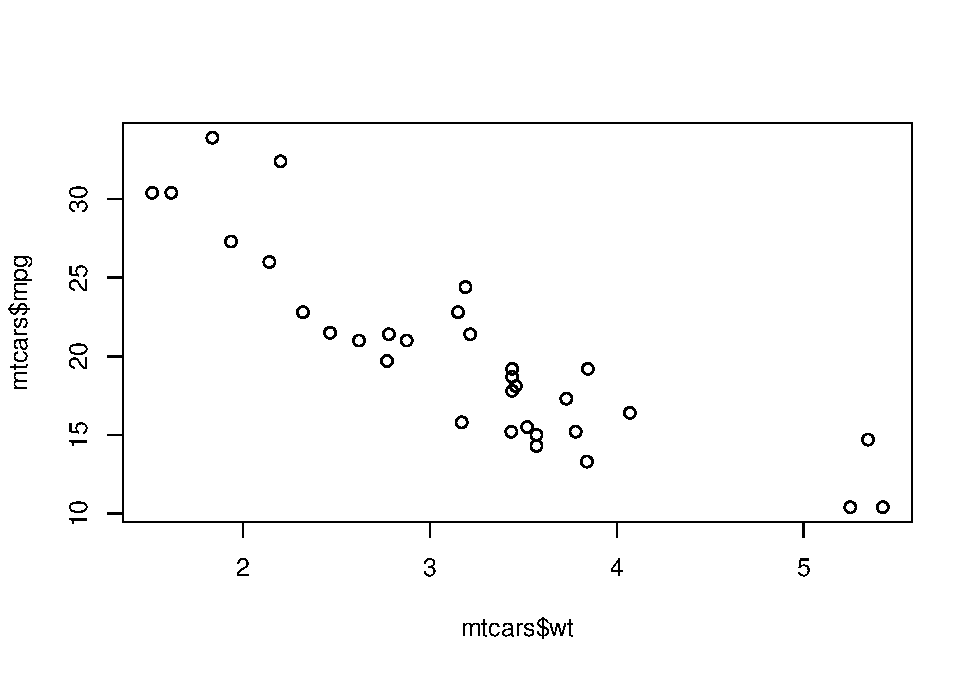
\includegraphics{_main_files/figure-latex/unnamed-chunk-92-1.pdf}

\begin{Shaded}
\begin{Highlighting}[]
\CommentTok{\# com o ggplot2 faríamos}
\FunctionTok{qplot}\NormalTok{(wt, mpg, }\AttributeTok{data =}\NormalTok{ mtcars)}
\end{Highlighting}
\end{Shaded}

\begin{verbatim}
## Warning: `qplot()` was deprecated in ggplot2 3.4.0.
## This warning is displayed once every 8 hours.
## Call `lifecycle::last_lifecycle_warnings()` to see where this warning was
## generated.
\end{verbatim}

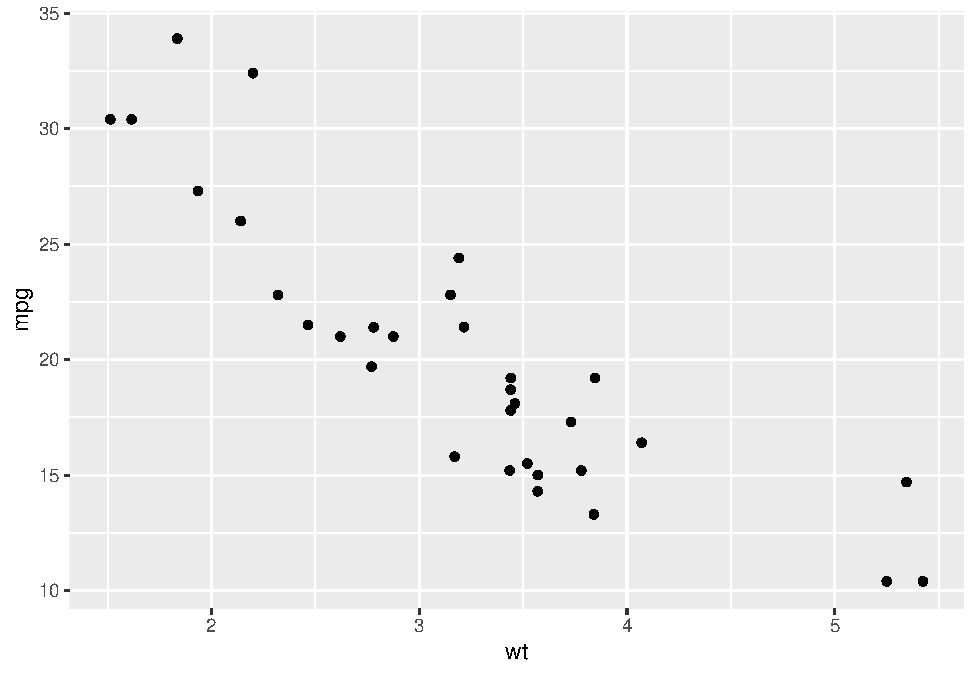
\includegraphics{_main_files/figure-latex/unnamed-chunk-92-2.pdf}

\hypertarget{criando-gruxe1ficos-de-linha}{%
\subsection{Criando gráficos de linha}\label{criando-gruxe1ficos-de-linha}}

Para fazer um gráfico em linha com a função plot, basta adicionar um outro argumento a função. Na janela de comando (Console) digite o código abaixo e atente para o argumento type = ``l''.

\begin{Shaded}
\begin{Highlighting}[]
\FunctionTok{plot}\NormalTok{(pressure}\SpecialCharTok{$}\NormalTok{temperature, pressure}\SpecialCharTok{$}\NormalTok{pressure, }\AttributeTok{type =} \StringTok{"l"}\NormalTok{)}

\CommentTok{\# para adicionar pontos e/ou múltiplas linhas, primeiramente}
\CommentTok{\# faz se o uso de plot() para a primeira linha e então usa{-}se}
\CommentTok{\# a função points() para pontos adicionais e lines() para}
\CommentTok{\# linhas adicionais}

\FunctionTok{plot}\NormalTok{(pressure}\SpecialCharTok{$}\NormalTok{temperature, pressure}\SpecialCharTok{$}\NormalTok{pressure, }\AttributeTok{type =} \StringTok{"l"}\NormalTok{)}
\FunctionTok{points}\NormalTok{(pressure}\SpecialCharTok{$}\NormalTok{temperature, pressure}\SpecialCharTok{$}\NormalTok{pressure)}
\FunctionTok{lines}\NormalTok{(pressure}\SpecialCharTok{$}\NormalTok{temperature, pressure}\SpecialCharTok{$}\NormalTok{pressure}\SpecialCharTok{/}\DecValTok{2}\NormalTok{, }\AttributeTok{col =} \StringTok{"red"}\NormalTok{)}
\FunctionTok{points}\NormalTok{(pressure}\SpecialCharTok{$}\NormalTok{temperature, pressure}\SpecialCharTok{$}\NormalTok{pressure}\SpecialCharTok{/}\DecValTok{2}\NormalTok{, }\AttributeTok{col =} \StringTok{"red"}\NormalTok{)}
\end{Highlighting}
\end{Shaded}

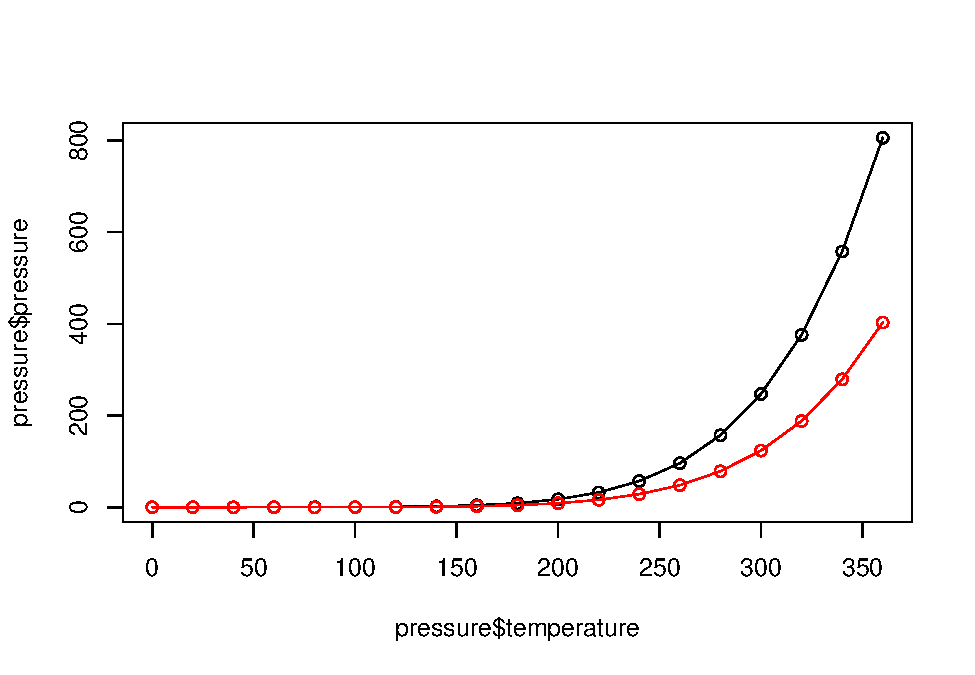
\includegraphics{_main_files/figure-latex/unnamed-chunk-93-1.pdf}

\begin{Shaded}
\begin{Highlighting}[]
\CommentTok{\# com o pacote ggplot2 fazemos uso da}
\CommentTok{\# função qplot(), concatenando linhas e pontos no mesmo vetor}
\CommentTok{\# da seguinte forma}

\FunctionTok{qplot}\NormalTok{(temperature, pressure, }\AttributeTok{data =}\NormalTok{ pressure, }\AttributeTok{geom =} \FunctionTok{c}\NormalTok{(}\StringTok{"line"}\NormalTok{,}
\StringTok{"point"}\NormalTok{))}
\end{Highlighting}
\end{Shaded}

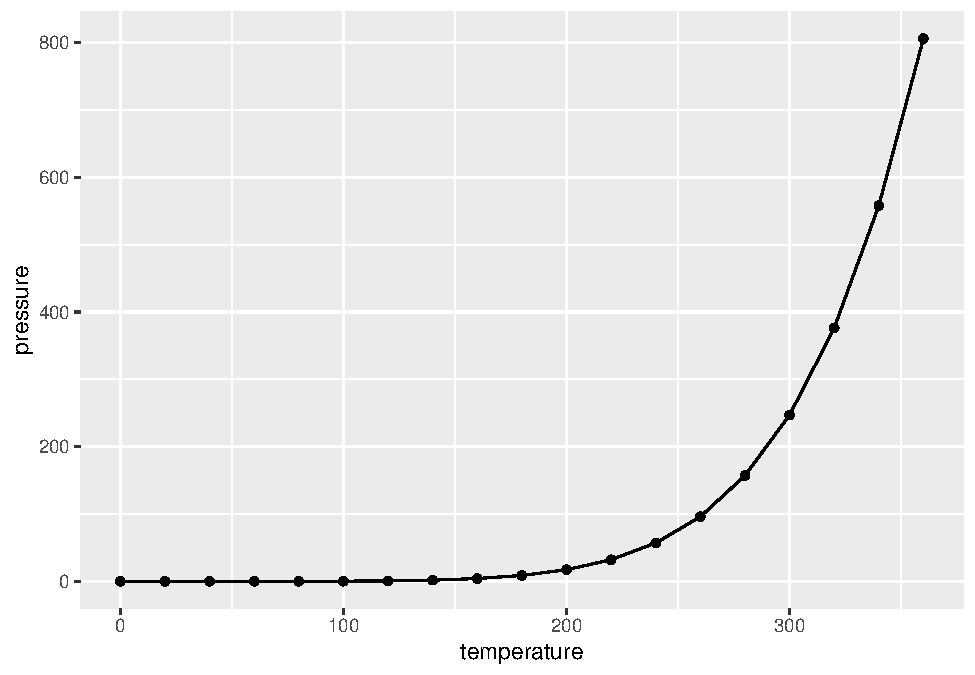
\includegraphics{_main_files/figure-latex/unnamed-chunk-93-2.pdf}

\hypertarget{criando-gruxe1ficos-de-barra}{%
\subsection{Criando gráficos de barra}\label{criando-gruxe1ficos-de-barra}}

A função utilizada para criar gráficos em barra é a \texttt{barplot()} e é utilizada passando-se o vetor de valores para a altura de cada barra como argumento da função e de modo opcional, outro argumento que também é utilizado é o vetor de labels para cada barra. As vezes, gráficos em barra se referem a gráficos onde as barras representam a quantidade de casos em cada categoria. Para gerar a quantia de cada valor único em um vetor, usa-se a função \texttt{table()}.

\begin{Shaded}
\begin{Highlighting}[]
\FunctionTok{table}\NormalTok{(mtcars}\SpecialCharTok{$}\NormalTok{cyl)}
\end{Highlighting}
\end{Shaded}

\begin{verbatim}
## 
##  4  6  8 
## 11  7 14
\end{verbatim}

\begin{Shaded}
\begin{Highlighting}[]
\DocumentationTok{\#\#}
\DocumentationTok{\#\# 4 6 8}
\DocumentationTok{\#\# 11 7 14}
\CommentTok{\# o que significa que há 11 casos do valor 4, 7 casos do}
\CommentTok{\# valor 6 e 14 casos do valor 8}

\CommentTok{\# para gerar um gráfico em barra dessas quantias basta passar}
\CommentTok{\# como argumento para a função barplot()}
\FunctionTok{barplot}\NormalTok{(}\FunctionTok{table}\NormalTok{(mtcars}\SpecialCharTok{$}\NormalTok{cyl))}
\end{Highlighting}
\end{Shaded}

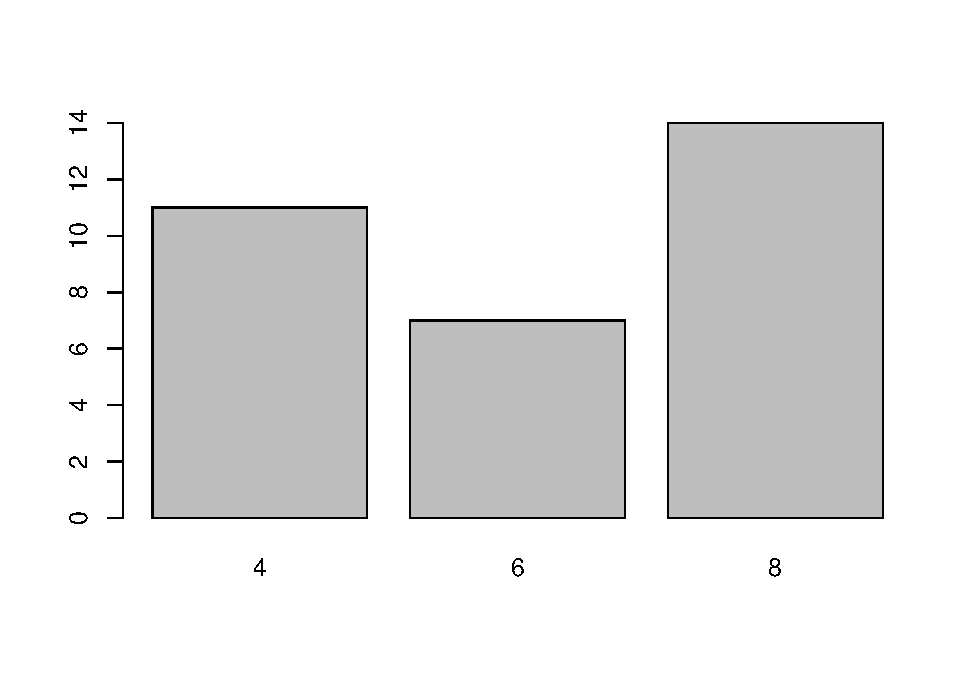
\includegraphics{_main_files/figure-latex/unnamed-chunk-94-1.pdf}

\hypertarget{criando-histogramas}{%
\subsection{Criando histogramas}\label{criando-histogramas}}

Para histogramas faz-se uso da função \texttt{hist()} passando como argumento o vetor de valores.

\begin{Shaded}
\begin{Highlighting}[]
\FunctionTok{hist}\NormalTok{(mtcars}\SpecialCharTok{$}\NormalTok{mpg)}
\end{Highlighting}
\end{Shaded}

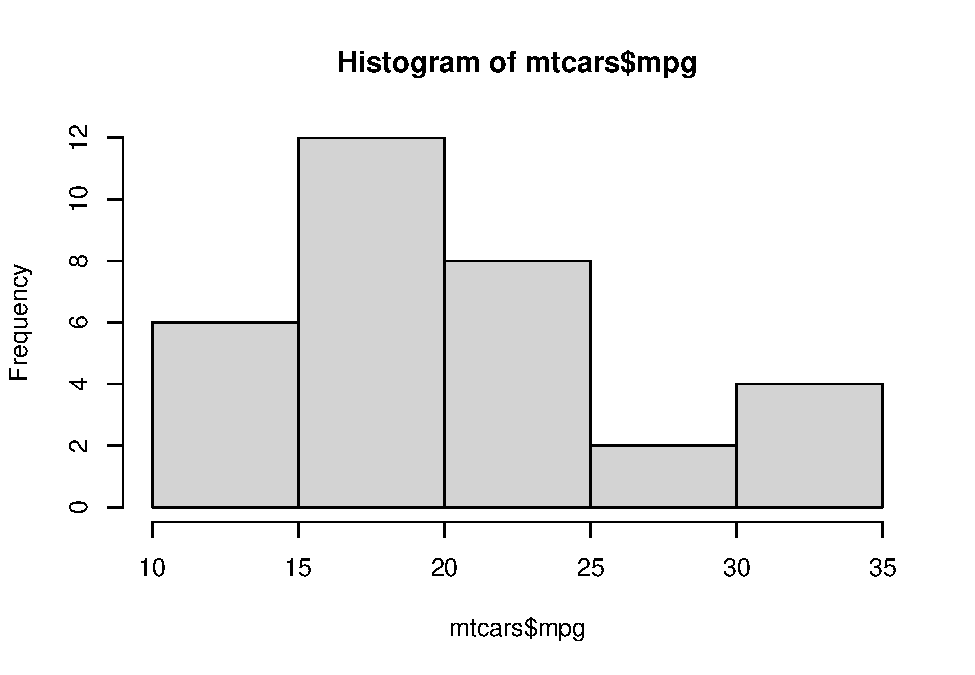
\includegraphics{_main_files/figure-latex/unnamed-chunk-95-1.pdf}

\begin{Shaded}
\begin{Highlighting}[]
\CommentTok{\# para especificar o número de quebras usa{-}se o argumento}
\CommentTok{\# breaks}
\FunctionTok{hist}\NormalTok{(mtcars}\SpecialCharTok{$}\NormalTok{mpg, }\AttributeTok{breaks =} \DecValTok{10}\NormalTok{)}
\end{Highlighting}
\end{Shaded}

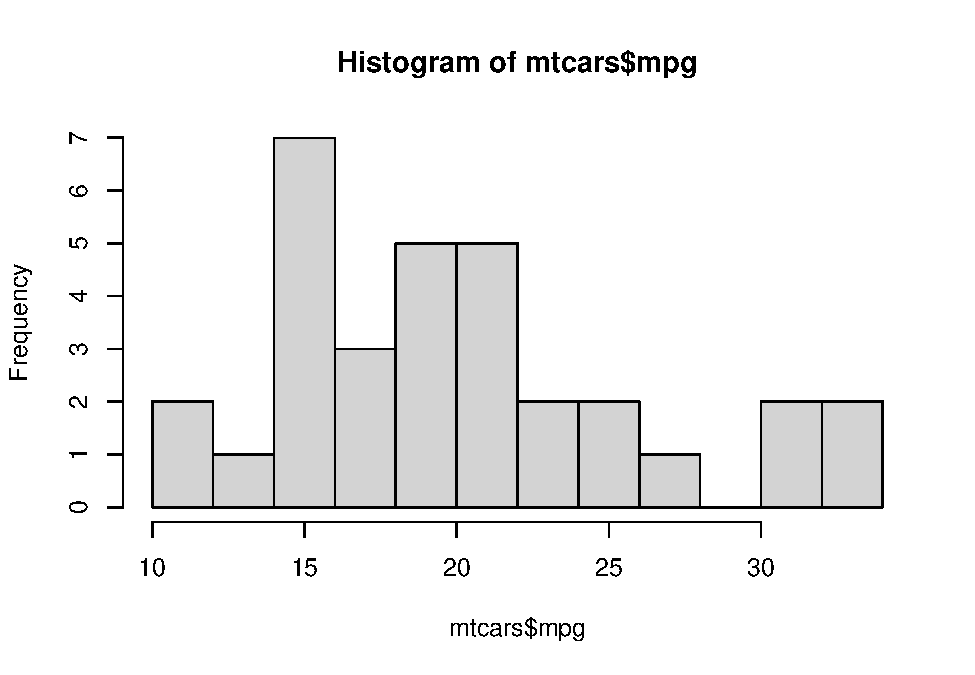
\includegraphics{_main_files/figure-latex/unnamed-chunk-95-2.pdf}

\hypertarget{criando-boxplot}{%
\subsection{Criando boxplot}\label{criando-boxplot}}

O gráfico do tipo boxplot é utilizado para comparar distribuições. Utiliza-se uma fórmula de sintaxe para combinar as variáveis a serem analisadas.

\begin{Shaded}
\begin{Highlighting}[]
\FunctionTok{boxplot}\NormalTok{(len }\SpecialCharTok{\textasciitilde{}}\NormalTok{ supp, }\AttributeTok{data =}\NormalTok{ ToothGrowth)}
\end{Highlighting}
\end{Shaded}

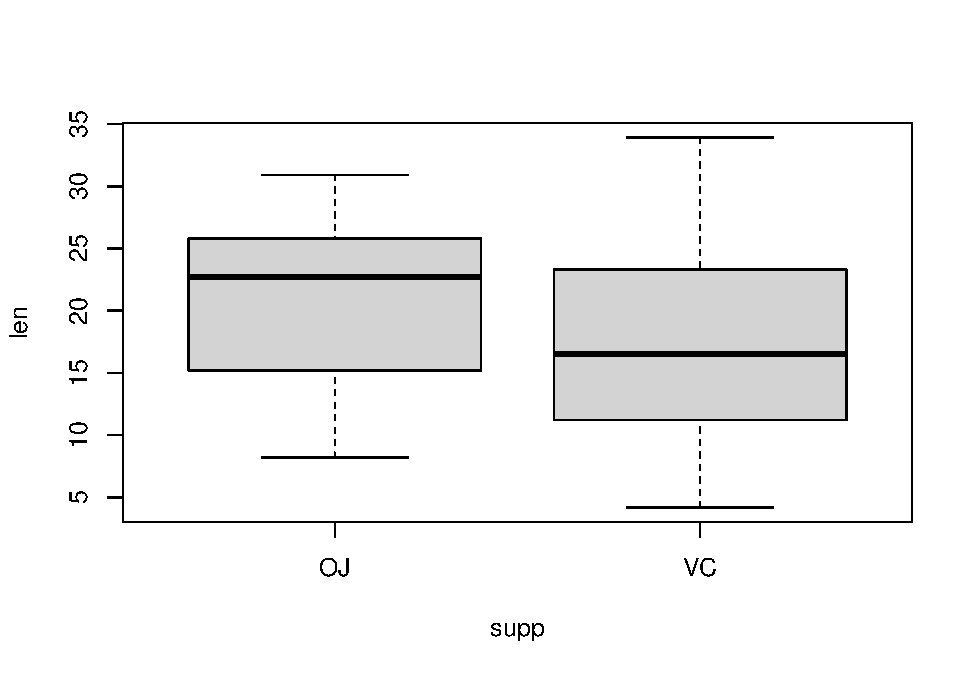
\includegraphics{_main_files/figure-latex/unnamed-chunk-96-1.pdf}

\begin{Shaded}
\begin{Highlighting}[]
\CommentTok{\# outra forma de obter o mesmo gráfico com o pacote ggplot2 é}
\FunctionTok{qplot}\NormalTok{(supp, len, }\AttributeTok{data =}\NormalTok{ ToothGrowth, }\AttributeTok{geom =} \StringTok{"boxplot"}\NormalTok{)}
\end{Highlighting}
\end{Shaded}

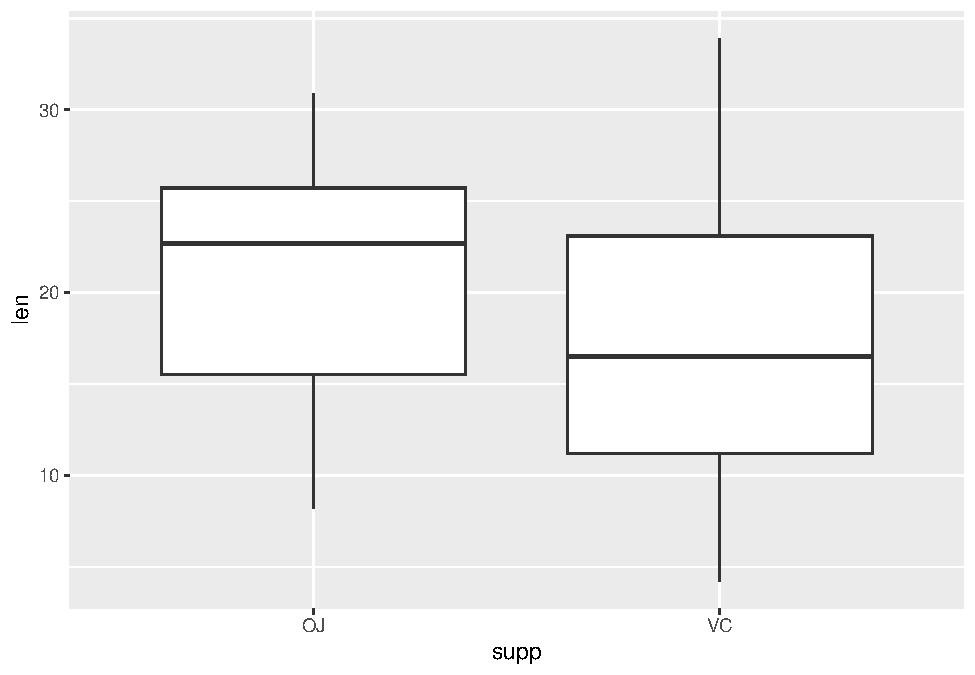
\includegraphics{_main_files/figure-latex/unnamed-chunk-96-2.pdf}

Ao longo desta primeira parte da aula pudemos observar que os gráficos em R são montados passo a passo. E que, caso se queira incrementar títulos, e especificar outros detalhes, isso pode ser feito com a adição de outros argumentos nas funções utilizadas para criar os gráficos. Para saber mais a respeito dos argumentos de cada função, basta fazer \texttt{?} seguido do nome da função ou através de \texttt{help(“nomedafuncao”)}.

\begin{Shaded}
\begin{Highlighting}[]
\CommentTok{\# \textasciigrave{}?\textasciigrave{}(plot)}
\CommentTok{\# help("plot")}

\FunctionTok{data}\NormalTok{(mtcars)}
\FunctionTok{head}\NormalTok{(mtcars)}
\end{Highlighting}
\end{Shaded}

\begin{verbatim}
##                    mpg cyl disp  hp drat    wt  qsec vs am gear carb
## Mazda RX4         21.0   6  160 110 3.90 2.620 16.46  0  1    4    4
## Mazda RX4 Wag     21.0   6  160 110 3.90 2.875 17.02  0  1    4    4
## Datsun 710        22.8   4  108  93 3.85 2.320 18.61  1  1    4    1
## Hornet 4 Drive    21.4   6  258 110 3.08 3.215 19.44  1  0    3    1
## Hornet Sportabout 18.7   8  360 175 3.15 3.440 17.02  0  0    3    2
## Valiant           18.1   6  225 105 2.76 3.460 20.22  1  0    3    1
\end{verbatim}

\begin{Shaded}
\begin{Highlighting}[]
\FunctionTok{plot}\NormalTok{(disp }\SpecialCharTok{\textasciitilde{}}\NormalTok{ mpg, }\AttributeTok{data =}\NormalTok{ mtcars, }\AttributeTok{main =} \StringTok{"My First Plot"}\NormalTok{)}
\end{Highlighting}
\end{Shaded}

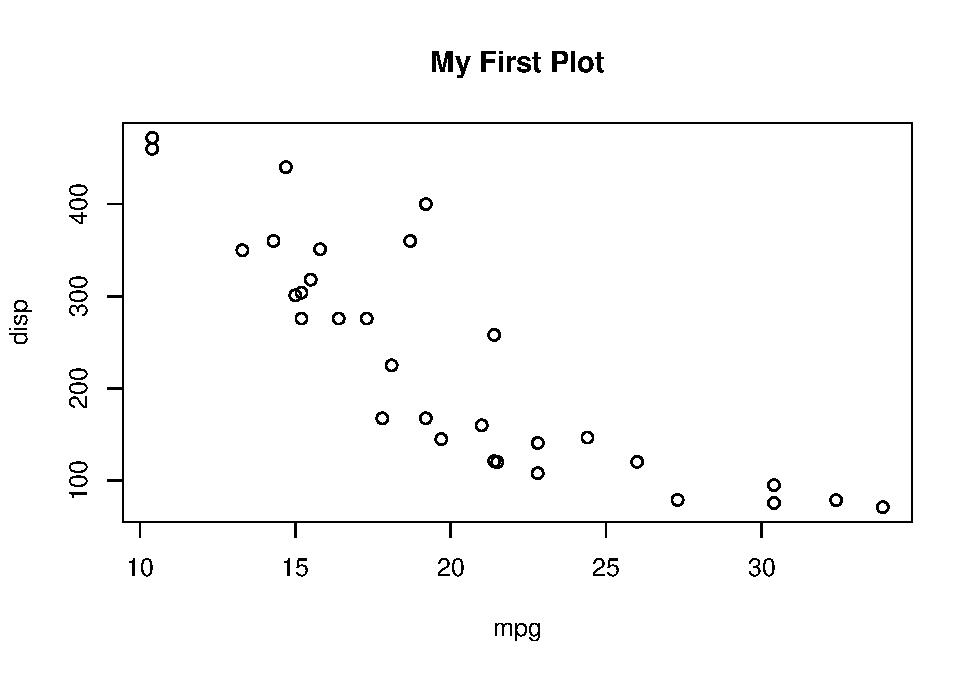
\includegraphics{_main_files/figure-latex/unnamed-chunk-97-1.pdf}

\hypertarget{lista-de-exercuxedcios-01}{%
\section{Lista de exercícios 01}\label{lista-de-exercuxedcios-01}}

\begin{enumerate}
\def\labelenumi{\arabic{enumi}.}
\item
  Utilizando o dataset cars, construa um gráfico com a função \texttt{plot()}. Mostre a
  relação entre as variáveis distância (dist) e velocidade (speed). Como título do gráfico coloque ``Relação entre distância e velocidade'' e, para as labels do eixo x e y, ``Velocidade (milhas por hora)'' e ``Distância percorrida (milhas)'', respectivamente. Os pontos do gráfico devem ser vermelhos.
\item
  A função \texttt{rnorm()} gera desvios aleatórios. Usando a ajuda, veja a documentação para essa função e exemplos de utilização. Comece com \texttt{rnorm(10)} e veja o que é retornado. Em seguida, usando a função \texttt{hist()} plote um histograma para visualizar a distribuição destes desvios aleatórios, agora com \texttt{rnorm(1000)}.
\item
  Utilizando o dataset airquality, use a função head() para ver quantas colunas
  contém o data set. Para selecionar uma coluna específica do dataset, usamos a notação ``\$''. Ou seja, se desejamos utilizar os dados contidos na camada ``Ozone'' devemos usar o seguinte comando airquality\$Ozone. Plote um histograma da coluna Ozone contida neste dataset, fazendo uso da notação \$.
\item
  Ainda utilizando o dataset airquality, agora vamos construir um boxplot. Plote um boxplot de Ozônio em função dos Meses, para o dataset airquality. Lembre-se de utilizar a sintaxe vista em aula \texttt{Ozone\ \textasciitilde{}\ Month}, ou seja, uma em função da outra, da mesma maneira que fazemos, y dependente de x \texttt{(y\ \textasciitilde{}\ x)}, neste caso, fazendo Ozone dependente de Month.
\item
  No boxplot do exercício anterior, os nomes dos eixos x e y não foram especificados e logo, não foram mostrados no gráfico. Como vimos, os gráficos em R são montados em etapas, com a adição de argumentos nas funções. Utilizando a seta para cima do teclado, recupere o comando digitado anteriormente e adicione novos argumentos. Defina o argumento \texttt{xlab} igual à ``Month'' e o argumento \texttt{ylab} igual à ``Ozone(ppb)''. Além destes, coloque também os argumentos \texttt{col.axis} igual à ``blue'' e \texttt{col.lab} igual à ``red'' e veja o que acontece com o seu boxplot.
\end{enumerate}

\hypertarget{ggplot2}{%
\section{GGPLOT2}\label{ggplot2}}

GGPlot2 é um pacote R disponível no repositório CRAN e pode ser instalado através da função install.packages(). Trata-se de uma implementação do conceito ``A Gramática dosGráficos'' criado por Leland Wilkinson e implementada por Hadley Wickham enquanto ele eraestudante de graduação na Universidade Estatal de Iowa. Uma gramática de gráficos representauma abstração de gráficos, ou seja, a teoria dos gráficos na qual conceitualiza peças básicas a partirdas quais você pode construir novos gráficos e objetos gráficos.

O pacote ggplot2 é composto por um conjunto de componentes independentes que podem
ser compostos de muitas diferentes formas. Utilizando este pacote você pode criar gráficos que sejam precisamente adaptados para o seu problema. Os componentes utilizados para construir um gráfico incluem estéticas (aesthetics) as quais são atributos como cor; forma; tamanho e objetos geométricos (geoms) tais como pontos, linhas e barras.

O pacote GGPlot2 possui duas funções principais, sendo elas \texttt{qplot()} e \texttt{ggplot()}. A função \texttt{qplot()} funciona como a função \texttt{plot()} base do R. Com a função \texttt{qplot()} é possível criar muitos tipos de plots (como gráficos de pontos, histogramas, boxplot). Já a função \texttt{ggplot()} é mais avançada, a qual é mais flexível e pode ser customizada para fazer coisas que a \texttt{qplot()} não faz. Vamos começar vendo a utilização da função \texttt{qplot()}.

Para isso vamos fazer uso de um dataset que vem com o pacote ggplot2, o dataset mpg. Este contém dados econômicos de combustível para 38 modelos de carros manufaturados em 1999 e 2008.

\begin{Shaded}
\begin{Highlighting}[]
\FunctionTok{library}\NormalTok{(ggplot2)}
\CommentTok{\# A utilização da função ésimilar as funções base para a}
\CommentTok{\# construção de gráficos Para montar um scatterplot, e}
\CommentTok{\# analisar a relação entre variáveis do data set como por}
\CommentTok{\# exemplo deslocamento do motor (displ) e milhas de rodovia}
\CommentTok{\# por galão (hwy) precisamos passar essas duas variáveis como}
\CommentTok{\# parâmetro na função e especificar o data set que contém}
\CommentTok{\# estas variáveis}
\FunctionTok{qplot}\NormalTok{(displ, hwy, }\AttributeTok{data =}\NormalTok{ mpg)}
\end{Highlighting}
\end{Shaded}

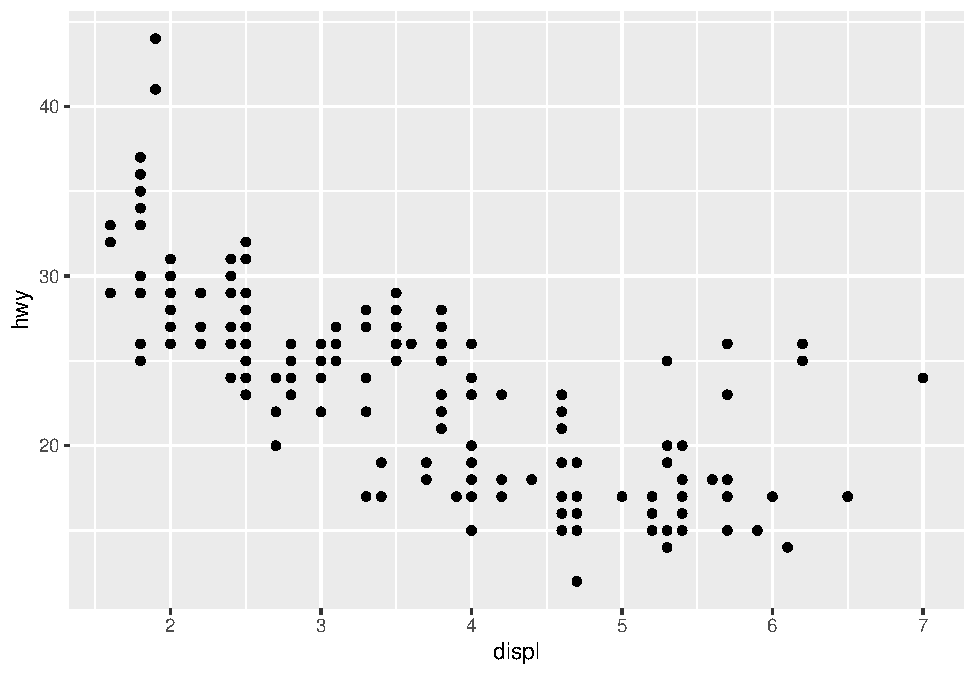
\includegraphics{_main_files/figure-latex/unnamed-chunk-98-1.pdf}

\begin{Shaded}
\begin{Highlighting}[]
\CommentTok{\# Supondo que gostaríamos de utilizar diferentes cores para}
\CommentTok{\# distinguir entre os 3 subconjuntos (fatores) tipos de}
\CommentTok{\# movimentação (drv) bastaria colocar um novo argumento,}
\CommentTok{\# conhecido como estética. Neste caso, cor, e definir igual a}
\CommentTok{\# drv}
\FunctionTok{qplot}\NormalTok{(displ, hwy, }\AttributeTok{data =}\NormalTok{ mpg, }\AttributeTok{color =}\NormalTok{ drv)}
\end{Highlighting}
\end{Shaded}

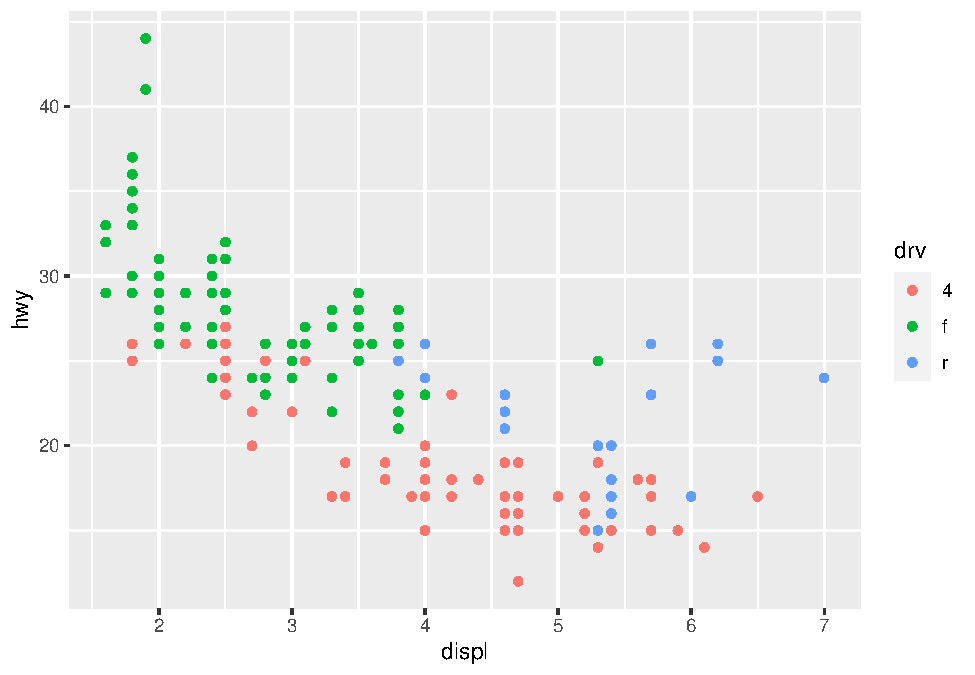
\includegraphics{_main_files/figure-latex/unnamed-chunk-98-2.pdf}

Utilizando o argumento geom (que se refere aos objetos geométricos) podemos especificar pontos, formas e até mesmo o tipo de gráfico que será plotado. Agora vamos construir um boxplot utilizando a função \texttt{qplot()}.

\begin{Shaded}
\begin{Highlighting}[]
\CommentTok{\# Primeiro especificamos a variável na qual queremos dividir}
\CommentTok{\# os dados (drv), para então em seguida, especificar a}
\CommentTok{\# variável na qual queremos examinar, neste caso hwy. O}
\CommentTok{\# terceiro argumento se refere ao dado (=mpg) e o quarto,}
\CommentTok{\# geom definido como a string \textquotesingle{}boxplot\textquotesingle{}}
\FunctionTok{qplot}\NormalTok{(drv, hwy, }\AttributeTok{data =}\NormalTok{ mpg, }\AttributeTok{geom =} \StringTok{"boxplot"}\NormalTok{)}
\end{Highlighting}
\end{Shaded}

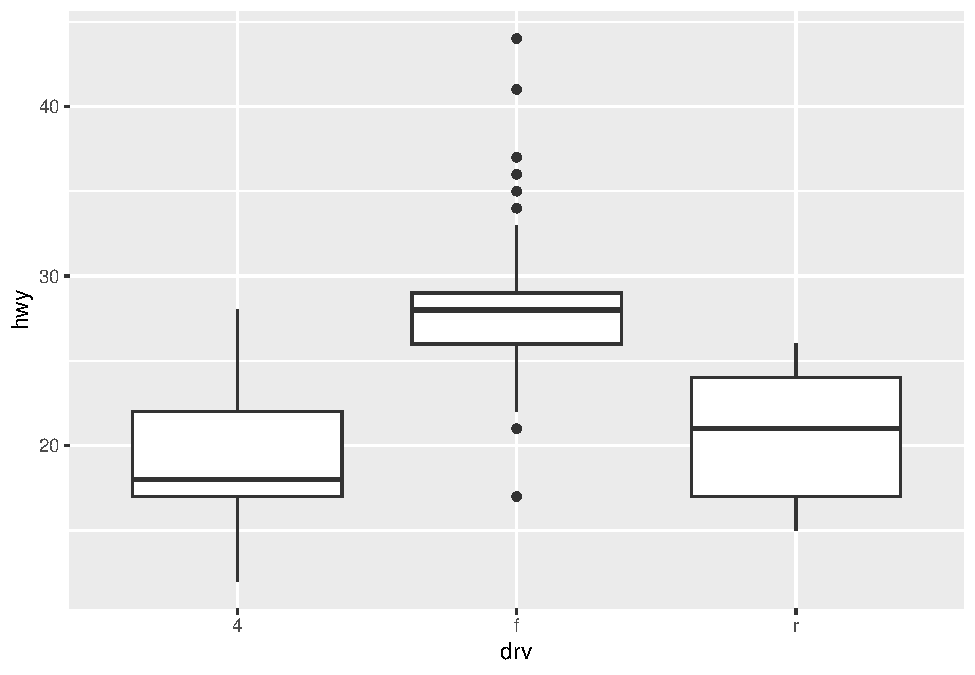
\includegraphics{_main_files/figure-latex/unnamed-chunk-99-1.pdf}

Com o código acima pudemos visualizar 3 boxes, um para cada tipo de movimentação. No entanto, podemos definir com cores, para cada marca, basta colocar um outro argumento ao código anterior, color igual a manufacturer.

\begin{Shaded}
\begin{Highlighting}[]
\FunctionTok{qplot}\NormalTok{(drv, hwy, }\AttributeTok{data =}\NormalTok{ mpg, }\AttributeTok{geom =} \StringTok{"boxplot"}\NormalTok{, }\AttributeTok{color =}\NormalTok{ manufacturer)}
\end{Highlighting}
\end{Shaded}

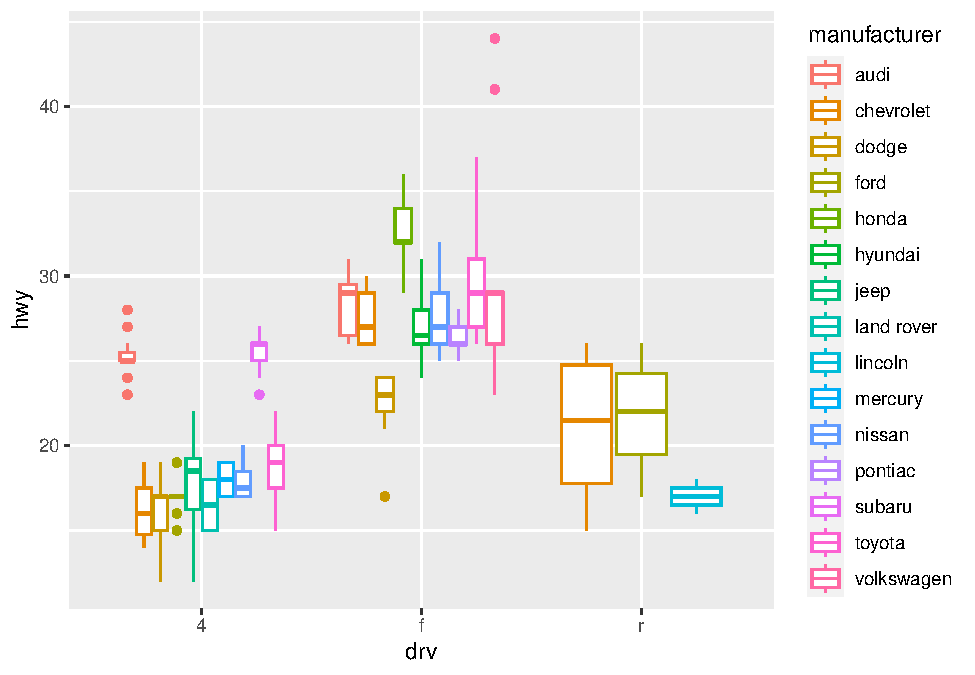
\includegraphics{_main_files/figure-latex/unnamed-chunk-100-1.pdf}

\begin{Shaded}
\begin{Highlighting}[]
\CommentTok{\# note que ainda temos 3 regiões nos gráficos,}
\CommentTok{\# correspondentes aos 3 tipos de movimentação, e em cada}
\CommentTok{\# temos subdivisões de acordo com as marcas}
\end{Highlighting}
\end{Shaded}

Agora depois de ver um pouco sobre a função \texttt{qplot()} iremos focar em alguns componentes fundamentais do pacote ggplot2. Para montar gráficos utilizando a função \texttt{ggplot()} vamos fazer em uma série de etapas. Isto com o intuito de analisar o que está acontecendo em cada passo até a obtenção do gráfico final. Primeiro iremos criar uma variável ``g'' e designar à esta uma chamada a função ggplot com 2 argumentos. O primeiro se refere a mpg (nosso data set em questão) e o segundo dirá a ggplot o que queremos plotar, que neste caso são as variáveis displ e hwy. Como estas se tratam das estéticas que queremos representar, passamos as mesmas como argumentos na função \texttt{aes}.

\begin{Shaded}
\begin{Highlighting}[]
\NormalTok{g }\OtherTok{\textless{}{-}} \FunctionTok{ggplot}\NormalTok{(mpg, }\FunctionTok{aes}\NormalTok{(displ, hwy))}

\CommentTok{\# o que ggplot fez foi criar um objeto gráfico o qual}
\CommentTok{\# designamos àvariável g O pacote ggplot2 precisa saber como}
\CommentTok{\# os dados serão visualizados, logo épreciso especificar.}
\CommentTok{\# Para criar um gráfico de pontos, podemos fazer por exemplo}

\NormalTok{g }\SpecialCharTok{+} \FunctionTok{geom\_point}\NormalTok{()}
\end{Highlighting}
\end{Shaded}

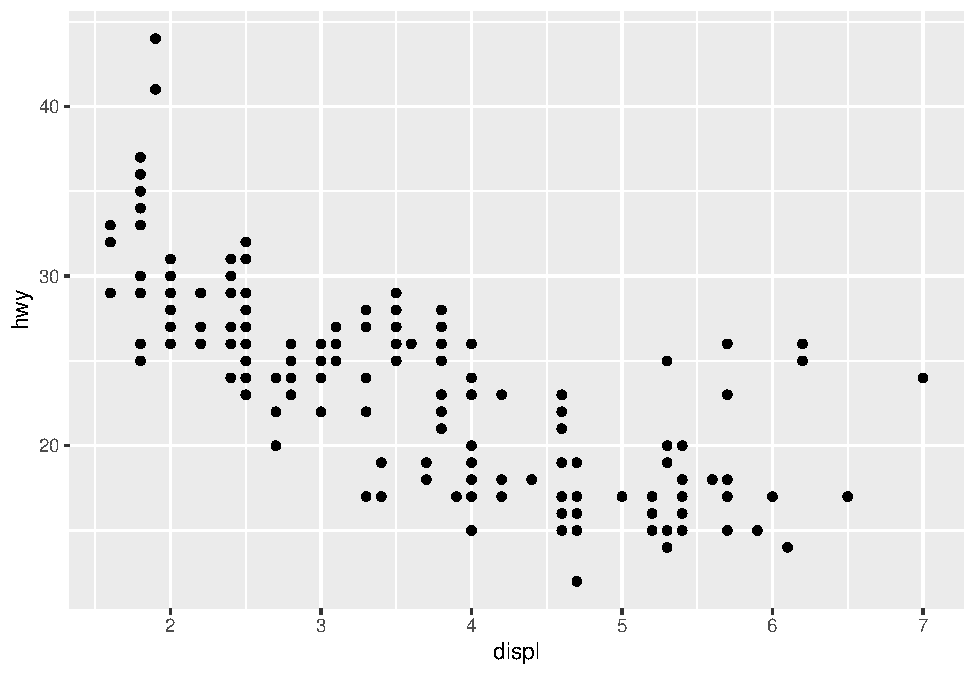
\includegraphics{_main_files/figure-latex/unnamed-chunk-101-1.pdf}

\begin{Shaded}
\begin{Highlighting}[]
\CommentTok{\# ao fazer chamada para a função geom\_point() foi adicionada}
\CommentTok{\# uma camada ao objeto gráfico. Perceba que você nao precisou}
\CommentTok{\# passar nenhum argumento para a função geom\_point(), isto}
\CommentTok{\# porque o objeto g já possui todo o dado armazenado nele.}
\CommentTok{\# Vamos agora adicionar outra camada, fazendo uma chamada}
\CommentTok{\# para a função geom\_smooth}

\NormalTok{g }\SpecialCharTok{+} \FunctionTok{geom\_point}\NormalTok{() }\SpecialCharTok{+} \FunctionTok{geom\_smooth}\NormalTok{()}
\end{Highlighting}
\end{Shaded}

\begin{verbatim}
## `geom_smooth()` using method = 'loess' and formula = 'y ~ x'
\end{verbatim}

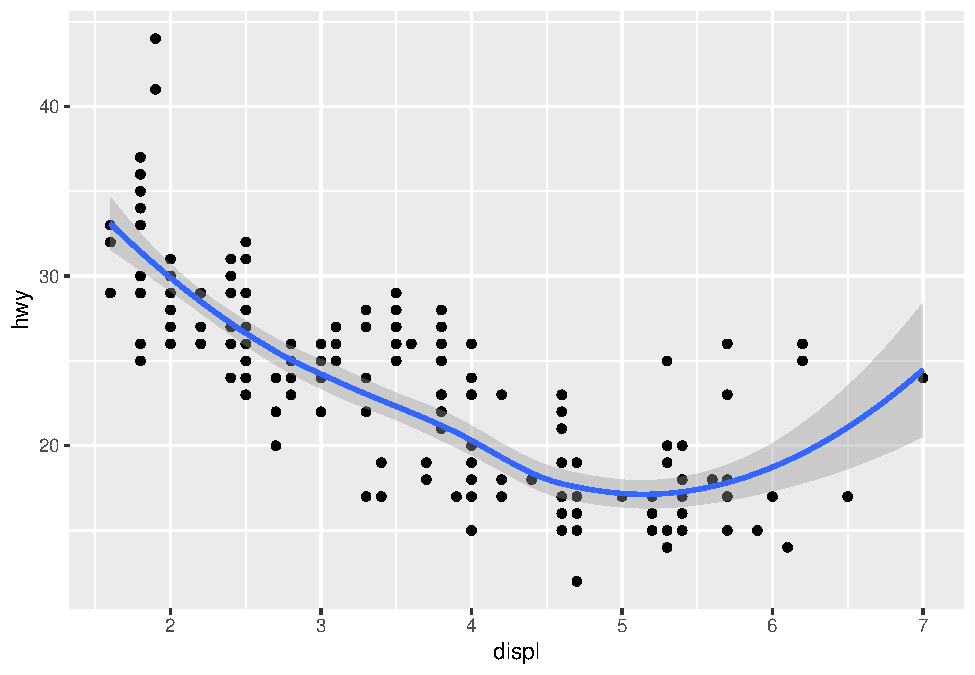
\includegraphics{_main_files/figure-latex/unnamed-chunk-101-2.pdf}

\begin{Shaded}
\begin{Highlighting}[]
\CommentTok{\# A sombra cinza ao redor da linha azul éo intervalo de}
\CommentTok{\# confiança. Épossível utilizar uma função diferente de}
\CommentTok{\# suavização, definindo método igual àlm (method = \textquotesingle{}lm\textquotesingle{})}
\end{Highlighting}
\end{Shaded}

Além das definições padrões, podemos adicionar outras anotações utilizando funções como \texttt{xlab()}, \texttt{ylab()} e \texttt{ggtitle()}. Vamos fazer um exemplo adicionando um título ao gráfico. Como por exemplo ``Meu GGPlot''.

\begin{Shaded}
\begin{Highlighting}[]
\NormalTok{g }\SpecialCharTok{+} \FunctionTok{geom\_point}\NormalTok{() }\SpecialCharTok{+} \FunctionTok{geom\_smooth}\NormalTok{(}\AttributeTok{method =} \StringTok{"lm"}\NormalTok{) }\SpecialCharTok{+} \FunctionTok{ggtitle}\NormalTok{(}\StringTok{"Meu GGPlot"}\NormalTok{)}
\end{Highlighting}
\end{Shaded}

\begin{verbatim}
## `geom_smooth()` using formula = 'y ~ x'
\end{verbatim}

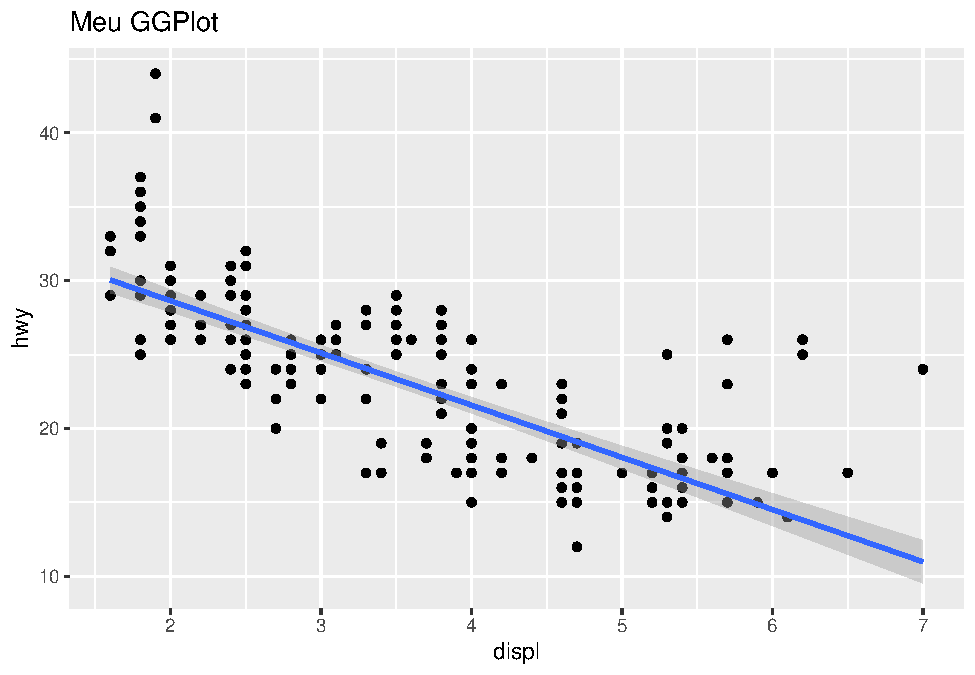
\includegraphics{_main_files/figure-latex/unnamed-chunk-102-1.pdf}

\begin{Shaded}
\begin{Highlighting}[]
\CommentTok{\# Podemos mudar outras estéticas do gráfico, ao definir cores}
\CommentTok{\# e tamanhos, por ex:}
\NormalTok{g }\SpecialCharTok{+} \FunctionTok{geom\_point}\NormalTok{(}\AttributeTok{color =} \StringTok{"pink"}\NormalTok{, }\AttributeTok{size =} \DecValTok{4}\NormalTok{, }\AttributeTok{alpha =} \DecValTok{1}\SpecialCharTok{/}\DecValTok{2}\NormalTok{)}
\end{Highlighting}
\end{Shaded}

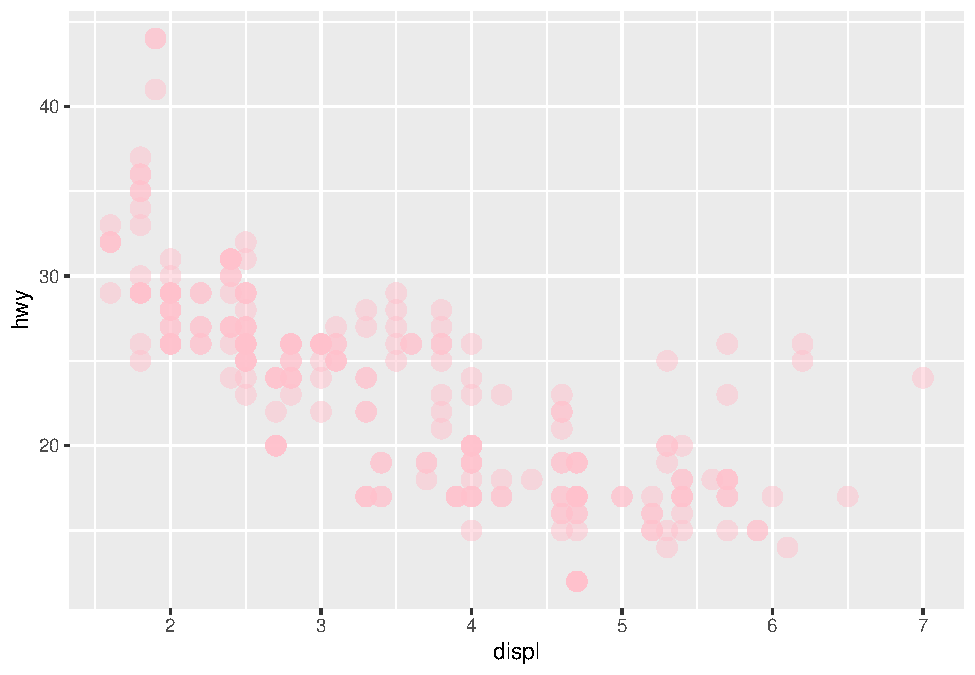
\includegraphics{_main_files/figure-latex/unnamed-chunk-102-2.pdf}

\begin{Shaded}
\begin{Highlighting}[]
\CommentTok{\# os diferentes tons de rosa são resultado do argumento}
\CommentTok{\# alpha, que diz o quão transparentes os pontos precisam ser.}
\CommentTok{\# Os círculos mais escuros indicam que há múltiplos pontos}
\end{Highlighting}
\end{Shaded}

\begin{Shaded}
\begin{Highlighting}[]
\NormalTok{g }\SpecialCharTok{+} \FunctionTok{geom\_point}\NormalTok{(}\FunctionTok{aes}\NormalTok{(}\AttributeTok{color =}\NormalTok{ drv)) }\SpecialCharTok{+} \FunctionTok{theme\_bw}\NormalTok{(}\AttributeTok{base\_family =} \StringTok{"Times"}\NormalTok{)}
\end{Highlighting}
\end{Shaded}

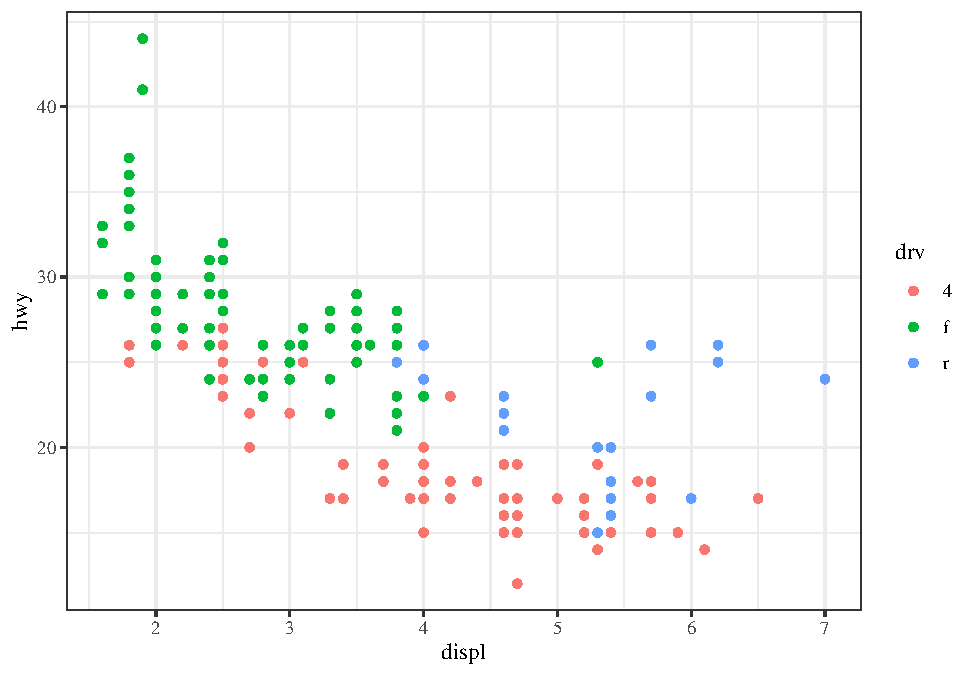
\includegraphics{_main_files/figure-latex/unnamed-chunk-103-1.pdf}

\hypertarget{exemplos-com-os-dados-de-tumor-de-mama-de-wiscosin}{%
\subsection{Exemplos com os dados de tumor de mama de Wiscosin}\label{exemplos-com-os-dados-de-tumor-de-mama-de-wiscosin}}

Nos exemplos abaixo, iremos utilizar novamente o data set com informações sobre nódulos de mama de Wiscosin. Vamos gerar gráficos utilizando as funções básicas do R e do GGplot. Alteramos algumas variáveis dos gráficos para apresentar algumas possibilidade de customização.

\begin{Shaded}
\begin{Highlighting}[]
\CommentTok{\# Vamos baixar os dados de características de nódulos de mama de Wiscosin}
\CommentTok{\# Mais informações sobre esse dataset em https://archive.ics.uci.edu/ml/datasets/Breast+Cancer+Wisconsin+\%28Diagnostic\%29}
\FunctionTok{download.file}\NormalTok{(}\AttributeTok{url =} \StringTok{\textquotesingle{}https://archive.ics.uci.edu/ml/machine{-}learning{-}databases/breast{-}cancer{-}wisconsin/wdbc.data\textquotesingle{}}\NormalTok{,}\AttributeTok{destfile =} \StringTok{"wbdc.data"}\NormalTok{)}

\CommentTok{\# Vamos importar os dados para o ambiente do R.}
\CommentTok{\# Os dados estão separados por vírgula, por isso o argumento sep=\textquotesingle{},\textquotesingle{}}
\CommentTok{\# outras opções e argumentos podem ser vistos em help(read.table)}
\NormalTok{brca }\OtherTok{\textless{}{-}} \FunctionTok{read.table}\NormalTok{(}\AttributeTok{file =} \StringTok{"./wbdc.data"}\NormalTok{, }\AttributeTok{sep =} \StringTok{\textquotesingle{},\textquotesingle{}}\NormalTok{)}
\FunctionTok{colnames}\NormalTok{(brca) }\OtherTok{\textless{}{-}} \FunctionTok{c}\NormalTok{(}\StringTok{\textquotesingle{}id\_number\textquotesingle{}}\NormalTok{, }\StringTok{\textquotesingle{}diagnosis\textquotesingle{}}\NormalTok{, }\StringTok{\textquotesingle{}radius\_mean\textquotesingle{}}\NormalTok{,}
                    \StringTok{\textquotesingle{}texture\_mean\textquotesingle{}}\NormalTok{, }\StringTok{\textquotesingle{}perimeter\_mean\textquotesingle{}}\NormalTok{, }\StringTok{\textquotesingle{}area\_mean\textquotesingle{}}\NormalTok{,}
                    \StringTok{\textquotesingle{}smoothness\_mean\textquotesingle{}}\NormalTok{, }\StringTok{\textquotesingle{}compactness\_mean\textquotesingle{}}\NormalTok{,}
                    \StringTok{\textquotesingle{}concavity\_mean\textquotesingle{}}\NormalTok{,}\StringTok{\textquotesingle{}concave\_points\_mean\textquotesingle{}}\NormalTok{,}
                    \StringTok{\textquotesingle{}symmetry\_mean\textquotesingle{}}\NormalTok{, }\StringTok{\textquotesingle{}fractal\_dimension\_mean\textquotesingle{}}\NormalTok{,}
                    \StringTok{\textquotesingle{}radius\_se\textquotesingle{}}\NormalTok{, }\StringTok{\textquotesingle{}texture\_se\textquotesingle{}}\NormalTok{, }\StringTok{\textquotesingle{}perimeter\_se\textquotesingle{}}\NormalTok{,}
                    \StringTok{\textquotesingle{}area\_se\textquotesingle{}}\NormalTok{, }\StringTok{\textquotesingle{}smoothness\_se\textquotesingle{}}\NormalTok{, }\StringTok{\textquotesingle{}compactness\_se\textquotesingle{}}\NormalTok{,}
                    \StringTok{\textquotesingle{}concavity\_se\textquotesingle{}}\NormalTok{, }\StringTok{\textquotesingle{}concave\_points\_se\textquotesingle{}}\NormalTok{,}
                    \StringTok{\textquotesingle{}symmetry\_se\textquotesingle{}}\NormalTok{, }\StringTok{\textquotesingle{}fractal\_dimension\_se\textquotesingle{}}\NormalTok{,}
                    \StringTok{\textquotesingle{}radius\_worst\textquotesingle{}}\NormalTok{, }\StringTok{\textquotesingle{}texture\_worst\textquotesingle{}}\NormalTok{,}
                    \StringTok{\textquotesingle{}perimeter\_worst\textquotesingle{}}\NormalTok{, }\StringTok{\textquotesingle{}area\_worst\textquotesingle{}}\NormalTok{,}
                    \StringTok{\textquotesingle{}smoothness\_worst\textquotesingle{}}\NormalTok{, }\StringTok{\textquotesingle{}compactness\_worst\textquotesingle{}}\NormalTok{,}
                    \StringTok{\textquotesingle{}concavity\_worst\textquotesingle{}}\NormalTok{, }\StringTok{\textquotesingle{}concave\_points\_worst\textquotesingle{}}\NormalTok{,}
                    \StringTok{\textquotesingle{}symmetry\_worst\textquotesingle{}}\NormalTok{, }\StringTok{\textquotesingle{}fractal\_dimension\_worst\textquotesingle{}}\NormalTok{)}
\NormalTok{brca}\SpecialCharTok{$}\NormalTok{diagnosis }\OtherTok{\textless{}{-}} \FunctionTok{as.factor}\NormalTok{(brca}\SpecialCharTok{$}\NormalTok{diagnosis)}
\CommentTok{\# Adicionar coluna com a razão do perímetro pelo raio dos nódulos}
\NormalTok{brca}\SpecialCharTok{$}\NormalTok{perimeter.radius }\OtherTok{\textless{}{-}}\NormalTok{ brca}\SpecialCharTok{$}\NormalTok{perimeter\_mean}\SpecialCharTok{/}\NormalTok{brca}\SpecialCharTok{$}\NormalTok{radius\_mean}
\end{Highlighting}
\end{Shaded}

\textbf{Histogramas}

\begin{Shaded}
\begin{Highlighting}[]
\CommentTok{\# Pacote básico}
\CommentTok{\# Em hist() por padrão usa{-}se contagem.}
\CommentTok{\# Para densidade, mudar argumento freq = F}
\FunctionTok{hist}\NormalTok{(brca}\SpecialCharTok{$}\NormalTok{radius\_mean, }\AttributeTok{breaks =} \DecValTok{20}\NormalTok{, }\AttributeTok{col =} \StringTok{"aquamarine"}\NormalTok{,}
     \AttributeTok{border =} \StringTok{"dodgerblue4"}\NormalTok{,}
     \AttributeTok{xlab =} \StringTok{"radius\_mean"}\NormalTok{, }\AttributeTok{ylab =} \StringTok{"Densidade"}\NormalTok{,}
     \AttributeTok{main =} \StringTok{"Raio médio de nódulos de mama"}\NormalTok{,}
     \AttributeTok{freq =}\NormalTok{ F)}
\CommentTok{\# Adicionar linha com a densidade}
\FunctionTok{lines}\NormalTok{(}\FunctionTok{density}\NormalTok{(brca}\SpecialCharTok{$}\NormalTok{radius\_mean), }\AttributeTok{col =} \StringTok{"red"}\NormalTok{)}
\end{Highlighting}
\end{Shaded}

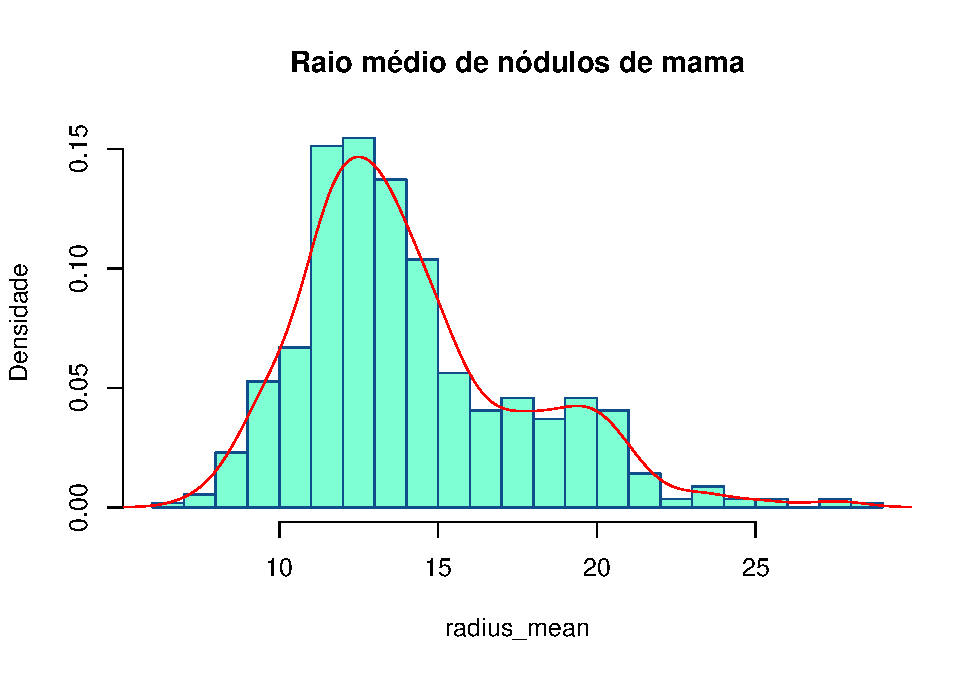
\includegraphics{_main_files/figure-latex/unnamed-chunk-105-1.pdf}

\begin{Shaded}
\begin{Highlighting}[]
\CommentTok{\# Salvar gráfico em PDF}
\CommentTok{\# https://r{-}coder.com/save{-}plot{-}r/}
\CommentTok{\# Nesse link tem outras opções (ex.; svg, pdf, jpeg, bmp, tiff)}
\FunctionTok{pdf}\NormalTok{(}\AttributeTok{file =} \StringTok{"./Meuplot.pdf"}\NormalTok{)}
\FunctionTok{hist}\NormalTok{(brca}\SpecialCharTok{$}\NormalTok{radius\_mean, }\AttributeTok{breaks =} \DecValTok{20}\NormalTok{, }\AttributeTok{col =} \StringTok{"aquamarine"}\NormalTok{,}
     \AttributeTok{border =} \StringTok{"dodgerblue4"}\NormalTok{,}
     \AttributeTok{xlab =} \StringTok{"Raio médio"}\NormalTok{, }\AttributeTok{ylab =} \StringTok{"Densidade"}\NormalTok{,}
     \AttributeTok{main =} \StringTok{"Raio médio de nódulos de mama"}\NormalTok{, }\AttributeTok{freq =}\NormalTok{ F)}
\FunctionTok{lines}\NormalTok{(}\FunctionTok{density}\NormalTok{(brca}\SpecialCharTok{$}\NormalTok{radius\_mean), }\AttributeTok{col =} \StringTok{"red"}\NormalTok{)}
\FunctionTok{dev.off}\NormalTok{()}
\end{Highlighting}
\end{Shaded}

\begin{verbatim}
## pdf 
##   2
\end{verbatim}

\begin{Shaded}
\begin{Highlighting}[]
\CommentTok{\# GGplot2}
\NormalTok{g }\OtherTok{\textless{}{-}} \FunctionTok{ggplot}\NormalTok{(}\AttributeTok{data =}\NormalTok{ brca, }\FunctionTok{aes}\NormalTok{(radius\_mean)) }\SpecialCharTok{+}
  \FunctionTok{geom\_histogram}\NormalTok{(}\AttributeTok{bins =} \DecValTok{20}\NormalTok{, }\AttributeTok{color =} \StringTok{"dodgerblue4"}\NormalTok{, }\AttributeTok{fill =} \StringTok{"aquamarine"}\NormalTok{,}
                 \FunctionTok{aes}\NormalTok{(}\AttributeTok{y =}\NormalTok{ ..density..)) }\SpecialCharTok{+}
  \FunctionTok{geom\_density}\NormalTok{(}\AttributeTok{color =} \StringTok{"red"}\NormalTok{) }\SpecialCharTok{+}
  \FunctionTok{labs}\NormalTok{(}\AttributeTok{title =} \StringTok{"Raio médio de nódulos de mama"}\NormalTok{)}
\NormalTok{g}
\end{Highlighting}
\end{Shaded}

\begin{verbatim}
## Warning: The dot-dot notation (`..density..`) was deprecated in ggplot2 3.4.0.
## i Please use `after_stat(density)` instead.
## This warning is displayed once every 8 hours.
## Call `lifecycle::last_lifecycle_warnings()` to see where this warning was
## generated.
\end{verbatim}

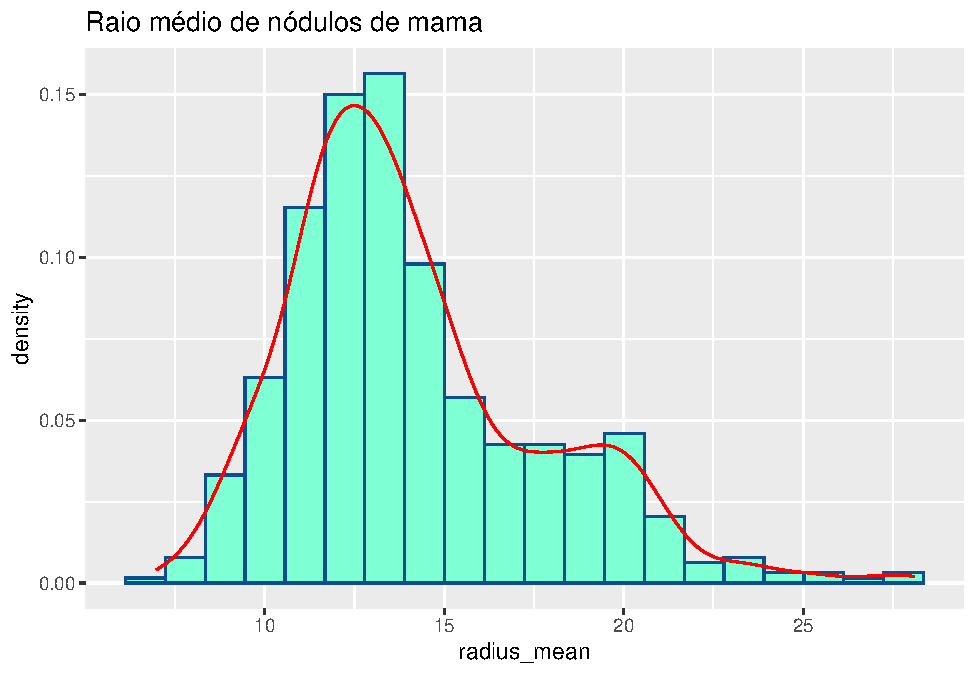
\includegraphics{_main_files/figure-latex/unnamed-chunk-105-2.pdf}

\begin{Shaded}
\begin{Highlighting}[]
\CommentTok{\# Mudando o tema e adicionando subtítulo}
\NormalTok{g }\SpecialCharTok{+} \FunctionTok{theme\_dark}\NormalTok{() }\SpecialCharTok{+}
  \FunctionTok{labs}\NormalTok{(}\AttributeTok{subtitle =} \StringTok{"Dados de Wiscosin"}\NormalTok{)}
\end{Highlighting}
\end{Shaded}

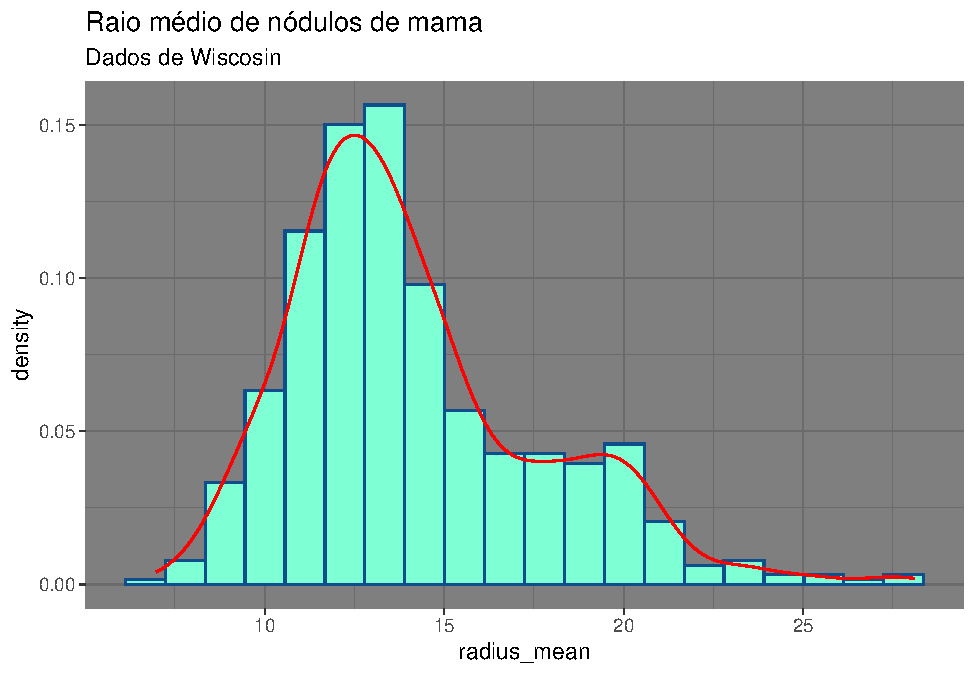
\includegraphics{_main_files/figure-latex/unnamed-chunk-105-3.pdf}

\begin{Shaded}
\begin{Highlighting}[]
\CommentTok{\# R base}
\FunctionTok{plot}\NormalTok{(brca}\SpecialCharTok{$}\NormalTok{radius\_mean, brca}\SpecialCharTok{$}\NormalTok{perimeter\_mean, }\AttributeTok{pch =} \DecValTok{15}\NormalTok{,}
     \AttributeTok{xlab =} \StringTok{"Raio médio"}\NormalTok{, }\AttributeTok{ylab =} \StringTok{"Perímetro médio"}\NormalTok{,}
     \AttributeTok{col =}\NormalTok{ brca}\SpecialCharTok{$}\NormalTok{diagnosis)}
\CommentTok{\# Adicionar legenda}
\CommentTok{\# https://statisticsglobe.com/add{-}legend{-}to{-}plot{-}in{-}base{-}r}
\FunctionTok{legend}\NormalTok{(}\StringTok{"topleft"}\NormalTok{, }\AttributeTok{legend =} \FunctionTok{c}\NormalTok{(}\StringTok{"B"}\NormalTok{,}\StringTok{"M"}\NormalTok{),}
       \AttributeTok{col =} \DecValTok{1}\SpecialCharTok{:}\DecValTok{2}\NormalTok{, }\AttributeTok{pch =} \DecValTok{15}\NormalTok{)}
\end{Highlighting}
\end{Shaded}

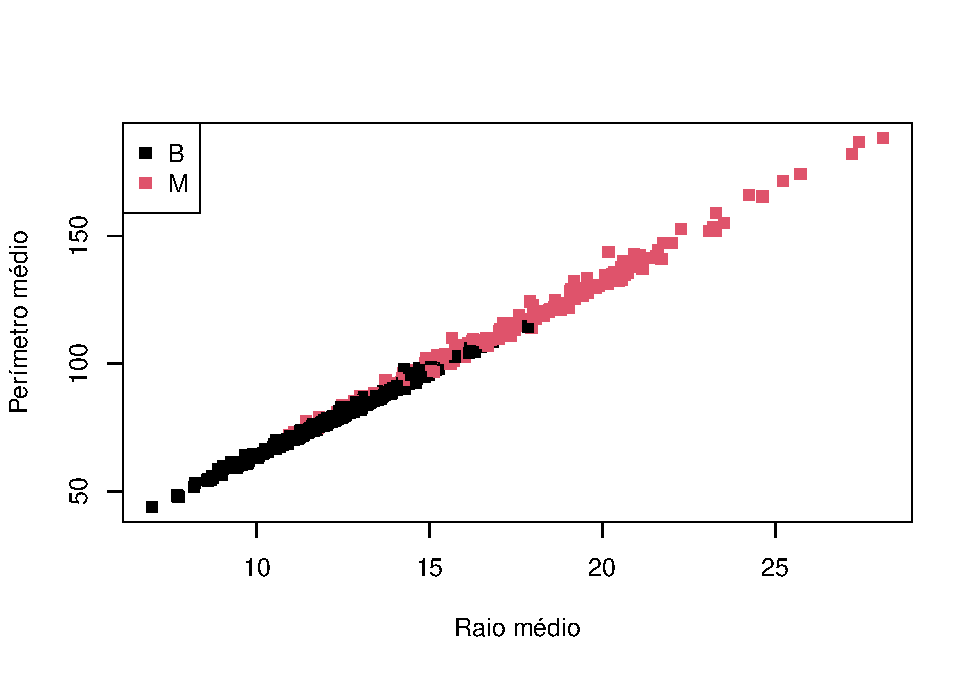
\includegraphics{_main_files/figure-latex/unnamed-chunk-105-4.pdf}

\begin{Shaded}
\begin{Highlighting}[]
\CommentTok{\# GGplot2}
\CommentTok{\# Criando variável categórica para area}
\CommentTok{\# Vamos utilizá{-}la para alterar a forma dos pontos no gráfico}
\FunctionTok{summary}\NormalTok{(brca}\SpecialCharTok{$}\NormalTok{area\_mean)}
\end{Highlighting}
\end{Shaded}

\begin{verbatim}
##    Min. 1st Qu.  Median    Mean 3rd Qu.    Max. 
##   143.5   420.3   551.1   654.9   782.7  2501.0
\end{verbatim}

\begin{Shaded}
\begin{Highlighting}[]
\NormalTok{brca}\SpecialCharTok{$}\NormalTok{Area }\OtherTok{\textless{}{-}}
  \FunctionTok{ifelse}\NormalTok{(brca}\SpecialCharTok{$}\NormalTok{area\_mean }\SpecialCharTok{\textless{}} \DecValTok{420}\NormalTok{,}
         \StringTok{"Baixo"}\NormalTok{,}
         \FunctionTok{ifelse}\NormalTok{(brca}\SpecialCharTok{$}\NormalTok{area\_mean }\SpecialCharTok{\textless{}} \DecValTok{750}\NormalTok{, }\StringTok{"Intermediário"}\NormalTok{, }\StringTok{"Alto"}\NormalTok{))}
\NormalTok{brca}\SpecialCharTok{$}\NormalTok{Area }\OtherTok{\textless{}{-}} \FunctionTok{factor}\NormalTok{(brca}\SpecialCharTok{$}\NormalTok{Area,}
                    \AttributeTok{levels =} \FunctionTok{c}\NormalTok{(}\StringTok{"Baixo"}\NormalTok{, }\StringTok{"Intermediário"}\NormalTok{, }\StringTok{"Alto"}\NormalTok{))}

\CommentTok{\# Agora os comandos para o gráfico em si}
\FunctionTok{ggplot}\NormalTok{(}\AttributeTok{data =}\NormalTok{ brca,}
       \FunctionTok{aes}\NormalTok{(}\AttributeTok{x=}\NormalTok{ radius\_mean, }\AttributeTok{y =}\NormalTok{ perimeter\_mean,}
           \AttributeTok{color =}\NormalTok{ diagnosis, }\AttributeTok{shape =}\NormalTok{ Area))}\SpecialCharTok{+}
  \FunctionTok{geom\_point}\NormalTok{()}\SpecialCharTok{+}
  \FunctionTok{labs}\NormalTok{(}\AttributeTok{x =} \StringTok{"Raio médio"}\NormalTok{,}
       \AttributeTok{y =} \StringTok{"Perímetro médio"}\NormalTok{,}
       \AttributeTok{color =} \StringTok{"Diagnóstico"}\NormalTok{,}
       \AttributeTok{shape =} \StringTok{"Área"}\NormalTok{)}\SpecialCharTok{+}
  \FunctionTok{scale\_fill\_discrete}\NormalTok{(}\AttributeTok{labels =} \FunctionTok{c}\NormalTok{(}\StringTok{"Benigno"}\NormalTok{, }\StringTok{"Maligno"}\NormalTok{))}
\end{Highlighting}
\end{Shaded}

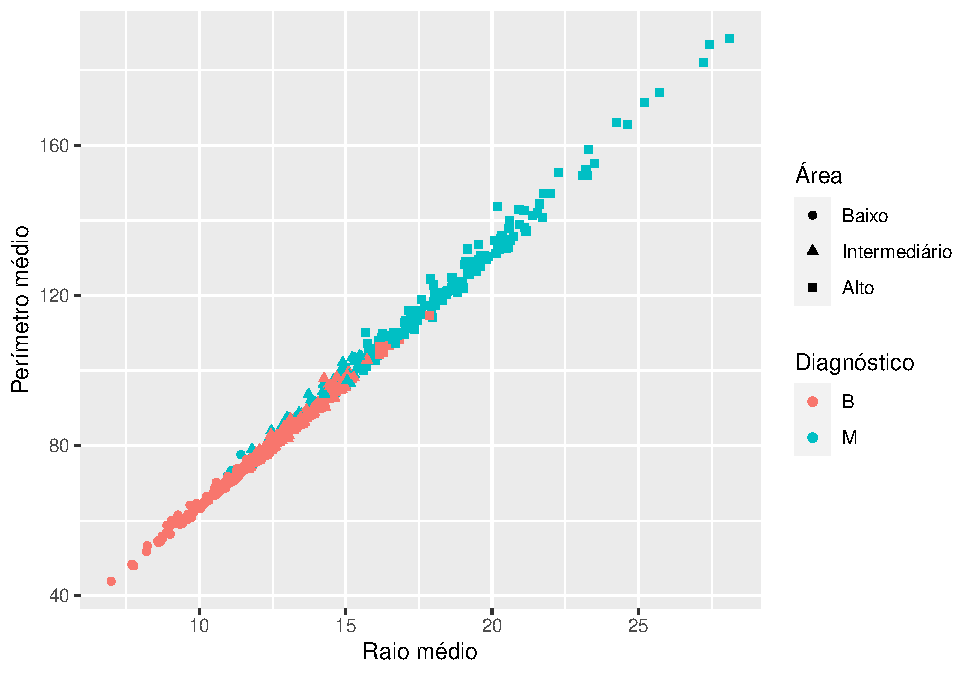
\includegraphics{_main_files/figure-latex/unnamed-chunk-105-5.pdf}

\textbf{Gráfico de barras}

\begin{Shaded}
\begin{Highlighting}[]
\CommentTok{\# Gráfico de barras}
\CommentTok{\# http://www.sthda.com/english/wiki/bar{-}plots{-}r{-}base{-}graphs}

\CommentTok{\# R base}
\FunctionTok{table}\NormalTok{(brca}\SpecialCharTok{$}\NormalTok{Area)}
\end{Highlighting}
\end{Shaded}

\begin{verbatim}
## 
##         Baixo Intermediário          Alto 
##           142           276           151
\end{verbatim}

\begin{Shaded}
\begin{Highlighting}[]
\NormalTok{counts }\OtherTok{\textless{}{-}} \FunctionTok{table}\NormalTok{(brca}\SpecialCharTok{$}\NormalTok{Area)}
\FunctionTok{barplot}\NormalTok{(counts, }\AttributeTok{col =} \FunctionTok{c}\NormalTok{(}\StringTok{"green"}\NormalTok{, }\StringTok{"orange"}\NormalTok{, }\StringTok{"red"}\NormalTok{))}
\end{Highlighting}
\end{Shaded}

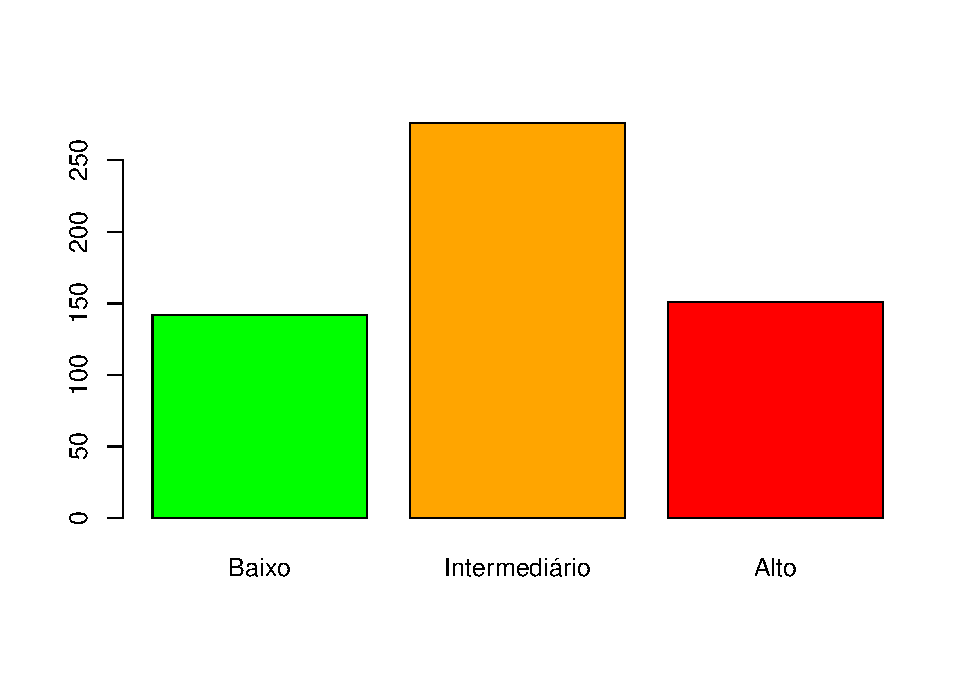
\includegraphics{_main_files/figure-latex/unnamed-chunk-106-1.pdf}

\begin{Shaded}
\begin{Highlighting}[]
\CommentTok{\# Ggplot2}
\CommentTok{\# http://www.sthda.com/english/wiki/ggplot2{-}barplots{-}quick{-}start{-}guide{-}r{-}software{-}and{-}data{-}visualization}
\FunctionTok{ggplot}\NormalTok{(brca,}
       \FunctionTok{aes}\NormalTok{(Area)) }\SpecialCharTok{+}
  \FunctionTok{geom\_bar}\NormalTok{(}\AttributeTok{stat=}\StringTok{"count"}\NormalTok{, }\FunctionTok{aes}\NormalTok{(}\AttributeTok{fill=}\NormalTok{Area))}
\end{Highlighting}
\end{Shaded}

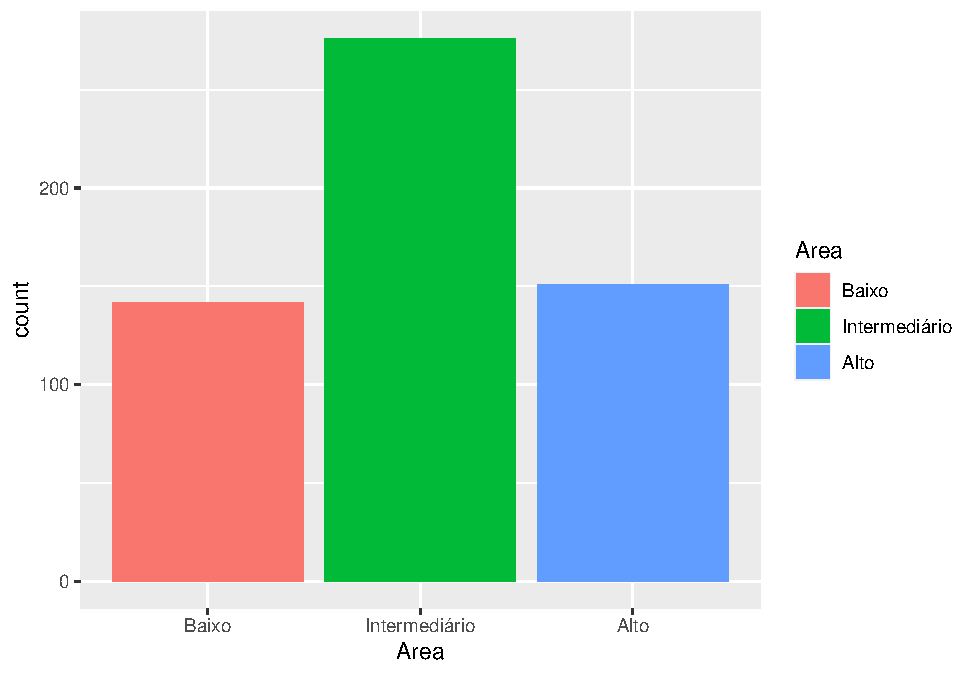
\includegraphics{_main_files/figure-latex/unnamed-chunk-106-2.pdf}

\textbf{Boxplot}

\begin{Shaded}
\begin{Highlighting}[]
\CommentTok{\# R base}
\CommentTok{\# https://statisticsglobe.com/boxplot{-}in{-}r}
\CommentTok{\# \textquotesingle{}\textasciitilde{}\textquotesingle{} éum operador para fórmular no R}
\CommentTok{\# Significa "depende de"}
\CommentTok{\# A aplicação évar\_dep \textasciitilde{} var\_ind}
\FunctionTok{boxplot}\NormalTok{(brca}\SpecialCharTok{$}\NormalTok{radius\_mean }\SpecialCharTok{\textasciitilde{}}\NormalTok{ brca}\SpecialCharTok{$}\NormalTok{diagnosis,}
        \AttributeTok{horizontal =}\NormalTok{ T, }\AttributeTok{las =} \DecValTok{1}\NormalTok{,}
        \AttributeTok{main =} \StringTok{"Raio médio e malignidade"}\NormalTok{,}
        \AttributeTok{col =} \FunctionTok{c}\NormalTok{(}\StringTok{"lightblue"}\NormalTok{, }\StringTok{"mistyrose"}\NormalTok{),}
        \AttributeTok{xlab =} \StringTok{"Raio médio"}\NormalTok{, }\AttributeTok{ylab =} \StringTok{""}\NormalTok{)}
\end{Highlighting}
\end{Shaded}

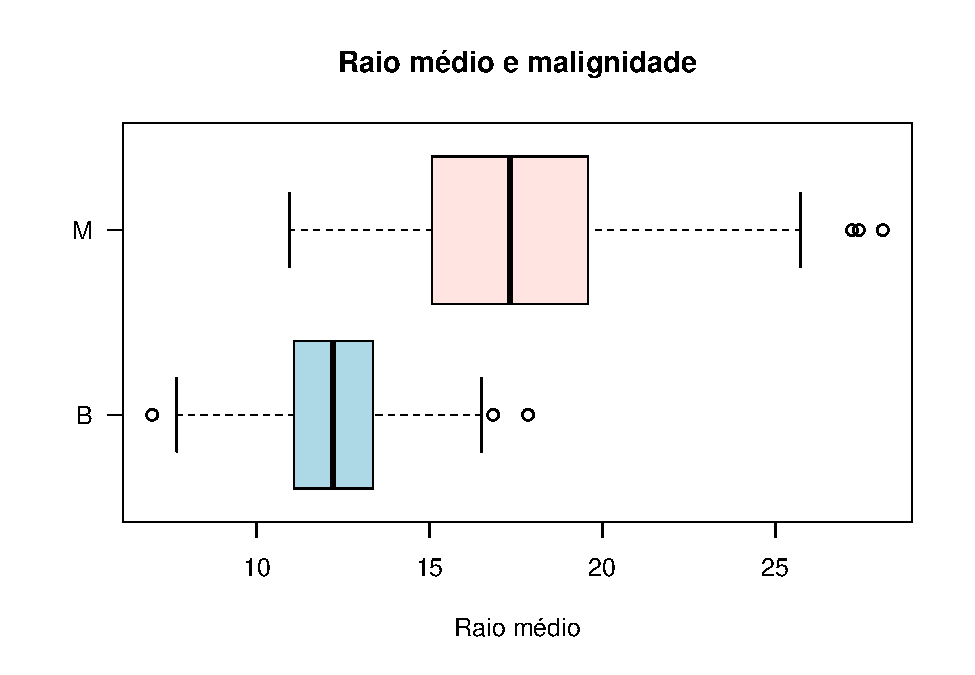
\includegraphics{_main_files/figure-latex/unnamed-chunk-107-1.pdf}

\begin{Shaded}
\begin{Highlighting}[]
\CommentTok{\# GGplot2}
\CommentTok{\# Criar boxplot e ajustar legenda}
\CommentTok{\# https://r{-}charts.com/ggplot2/legend/}
\NormalTok{g }\OtherTok{\textless{}{-}} \FunctionTok{ggplot}\NormalTok{(}\AttributeTok{data =}\NormalTok{ brca,}
            \FunctionTok{aes}\NormalTok{(}\AttributeTok{x=}\NormalTok{ diagnosis, }\AttributeTok{y =}\NormalTok{ radius\_mean, }\AttributeTok{fill =}\NormalTok{ diagnosis))}\SpecialCharTok{+}
  \FunctionTok{geom\_boxplot}\NormalTok{(}\AttributeTok{width =} \FloatTok{0.3}\NormalTok{) }\SpecialCharTok{+}
  \FunctionTok{labs}\NormalTok{(}\AttributeTok{x =} \StringTok{"Diagnóstico"}\NormalTok{,}
       \AttributeTok{y =} \StringTok{" Raio médio"}\NormalTok{,}
       \AttributeTok{fill =} \StringTok{"Legenda"}\NormalTok{) }\SpecialCharTok{+}
  \FunctionTok{scale\_x\_discrete}\NormalTok{(}\AttributeTok{labels =} \FunctionTok{c}\NormalTok{(}\StringTok{"BENIGNO"}\NormalTok{, }\StringTok{"MALIGNO"}\NormalTok{)) }\SpecialCharTok{+}
  \FunctionTok{scale\_fill\_discrete}\NormalTok{(}\AttributeTok{labels =} \FunctionTok{c}\NormalTok{(}\StringTok{"Benigno"}\NormalTok{, }\StringTok{"Maligno"}\NormalTok{))}\SpecialCharTok{+}
  \FunctionTok{theme}\NormalTok{(}\AttributeTok{legend.position =} \StringTok{"bottom"}\NormalTok{)}
\NormalTok{g}
\end{Highlighting}
\end{Shaded}

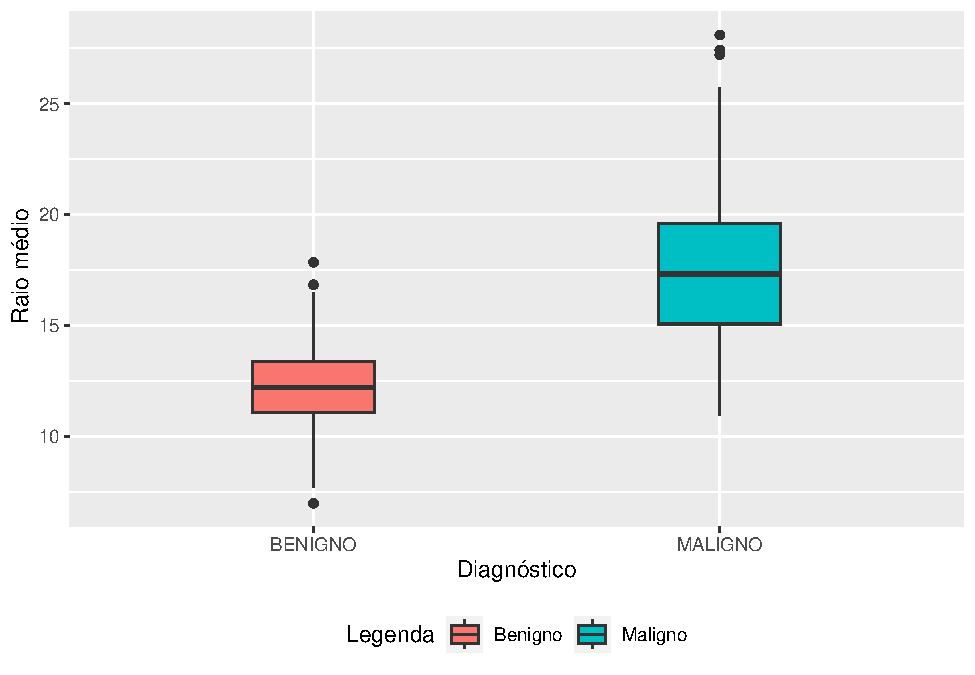
\includegraphics{_main_files/figure-latex/unnamed-chunk-107-2.pdf}

\begin{Shaded}
\begin{Highlighting}[]
\CommentTok{\# Adicionar violion plot}
\NormalTok{g }\OtherTok{\textless{}{-}}\NormalTok{ g }\SpecialCharTok{+} \FunctionTok{geom\_violin}\NormalTok{(}\AttributeTok{alpha =} \FloatTok{0.2}\NormalTok{)}
\NormalTok{g}
\end{Highlighting}
\end{Shaded}

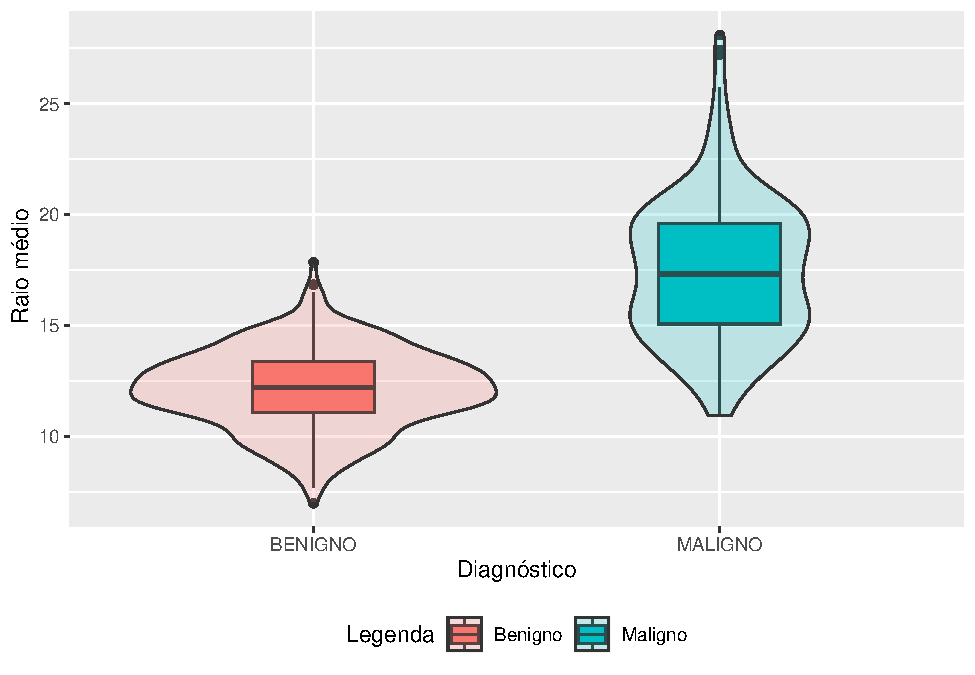
\includegraphics{_main_files/figure-latex/unnamed-chunk-107-3.pdf}

\begin{Shaded}
\begin{Highlighting}[]
\CommentTok{\# Para adicionar teste estatístico}
\CommentTok{\# http://sthda.com/english/articles/24{-}ggpubr{-}publication{-}ready{-}plots/76{-}add{-}p{-}values{-}and{-}significance{-}levels{-}to{-}ggplots/}
\CommentTok{\# Instalar pacote ggpubr caso não esteja instalado}
\FunctionTok{install.packages}\NormalTok{(}\StringTok{"ggpubr"}\NormalTok{)}
\end{Highlighting}
\end{Shaded}

\begin{verbatim}
## Installing package into '/home/jeanresende/R/x86_64-pc-linux-gnu-library/4.3'
## (as 'lib' is unspecified)
\end{verbatim}

\begin{Shaded}
\begin{Highlighting}[]
\CommentTok{\# Carregar pacote}
\FunctionTok{library}\NormalTok{(}\StringTok{"ggpubr"}\NormalTok{)}
\CommentTok{\# Adicionar teste estatístico ao gráfico}
\NormalTok{g }\SpecialCharTok{+}
\FunctionTok{stat\_compare\_means}\NormalTok{(}\AttributeTok{method =} \StringTok{"t.test"}\NormalTok{, }\AttributeTok{label =} \StringTok{"p.signif"}\NormalTok{,}
\AttributeTok{comparisons =} \FunctionTok{list}\NormalTok{(}\FunctionTok{c}\NormalTok{(}\StringTok{"B"}\NormalTok{, }\StringTok{"M"}\NormalTok{)))}
\end{Highlighting}
\end{Shaded}

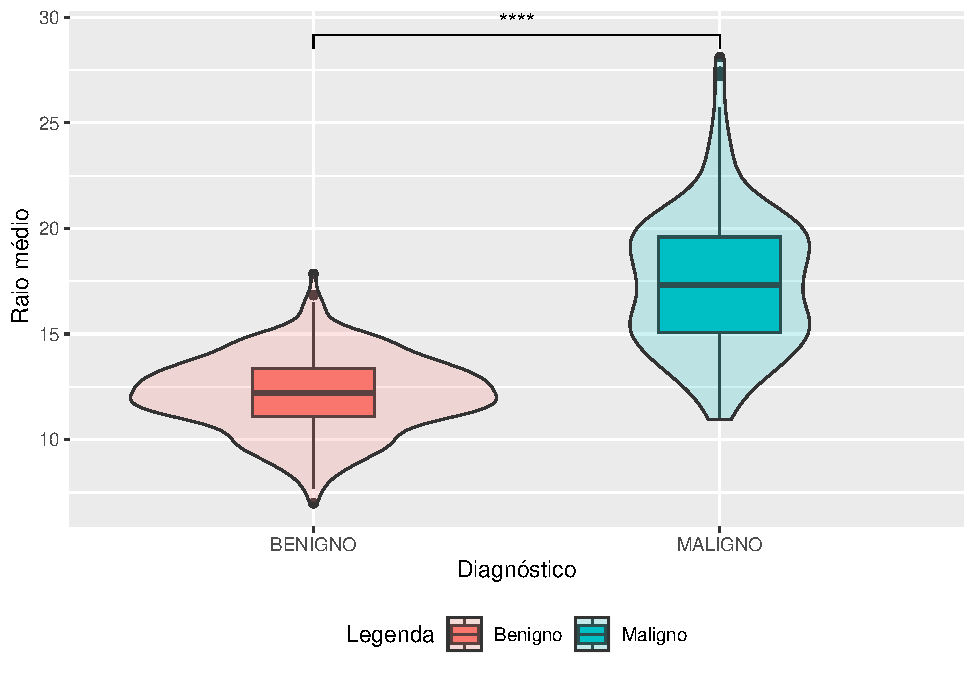
\includegraphics{_main_files/figure-latex/unnamed-chunk-107-4.pdf}

\hypertarget{bonus-track---gruxe1ficos-interativos-com-plotly}{%
\section{Bonus track - Gráficos interativos com plotly}\label{bonus-track---gruxe1ficos-interativos-com-plotly}}

O pacote plotly é uma forma bastante simples de se produzir gráficos interativos. Ele apresenta uma sintaxe própria que pode ser aprendida nas descrições das funções, no site oficial do pacote (\url{https://plotly.com/r/}) ou em vários tutoriais online. Aqui vamos apenas apresentar uma facilidade que o pacote traz a qual é sua compatibilidade com gráficos gerados pelo ggplot2. A função ggplotly() recebe um gráfico do ggplot e torna-o interativo. Essa função é compatível com a maior parte dos recursos do ggplot, apesar de existirem algumas poucas exceções. Além disso, os gráficos interativos gerados pelo plotly são compatíveis com o pacote shiny, podendo ser usado em dashboards e web apps. Abaixo vamos apresentar 2 exemplos simples transformando gráficos gerados com o ggplot em interativos.

\begin{Shaded}
\begin{Highlighting}[]
\CommentTok{\#install.packages("plotly")}
\FunctionTok{library}\NormalTok{(plotly)}
\end{Highlighting}
\end{Shaded}

\begin{verbatim}
## 
## Attaching package: 'plotly'
\end{verbatim}

\begin{verbatim}
## The following object is masked from 'package:ggplot2':
## 
##     last_plot
\end{verbatim}

\begin{verbatim}
## The following object is masked from 'package:stats':
## 
##     filter
\end{verbatim}

\begin{verbatim}
## The following object is masked from 'package:graphics':
## 
##     layout
\end{verbatim}

\begin{Shaded}
\begin{Highlighting}[]
\CommentTok{\# Criando um histograma com ggplot}
\NormalTok{g}\OtherTok{\textless{}{-}}\FunctionTok{ggplot}\NormalTok{(}\AttributeTok{data =}\NormalTok{ brca, }\FunctionTok{aes}\NormalTok{(radius\_mean)) }\SpecialCharTok{+}
  \FunctionTok{geom\_histogram}\NormalTok{(}\AttributeTok{bins =} \DecValTok{20}\NormalTok{, }\AttributeTok{color =} \StringTok{"dodgerblue4"}\NormalTok{, }\AttributeTok{fill =} \StringTok{"aquamarine"}\NormalTok{,}
                 \FunctionTok{aes}\NormalTok{(}\AttributeTok{y =}\NormalTok{ ..density..)) }\SpecialCharTok{+}
  \FunctionTok{geom\_density}\NormalTok{(}\AttributeTok{color =} \StringTok{"red"}\NormalTok{) }\SpecialCharTok{+}
  \FunctionTok{labs}\NormalTok{(}\AttributeTok{title =} \StringTok{"Raio médio de nódulos de mama"}\NormalTok{,}
       \AttributeTok{x =} \StringTok{"Raio médio"}\NormalTok{,}
       \AttributeTok{y =} \StringTok{"Densidade"}\NormalTok{,}
       \AttributeTok{subtitle =} \StringTok{"Dados de Wiscosin"}\NormalTok{)}\SpecialCharTok{+}
  \FunctionTok{theme}\NormalTok{(}\AttributeTok{axis.title.y =} \FunctionTok{element\_text}\NormalTok{(}\AttributeTok{face =} \StringTok{"bold"}\NormalTok{, }\AttributeTok{color=} \StringTok{"red"}\NormalTok{),}
        \AttributeTok{panel.background =} \FunctionTok{element\_rect}\NormalTok{(}\AttributeTok{fill =} \StringTok{"lightblue"}\NormalTok{))}

\CommentTok{\# Tornando{-}o interativo:}
\FunctionTok{ggplotly}\NormalTok{(g)}
\end{Highlighting}
\end{Shaded}

\begin{verbatim}
## PhantomJS not found. You can install it with webshot::install_phantomjs(). If it is installed, please make sure the phantomjs executable can be found via the PATH variable.
\end{verbatim}

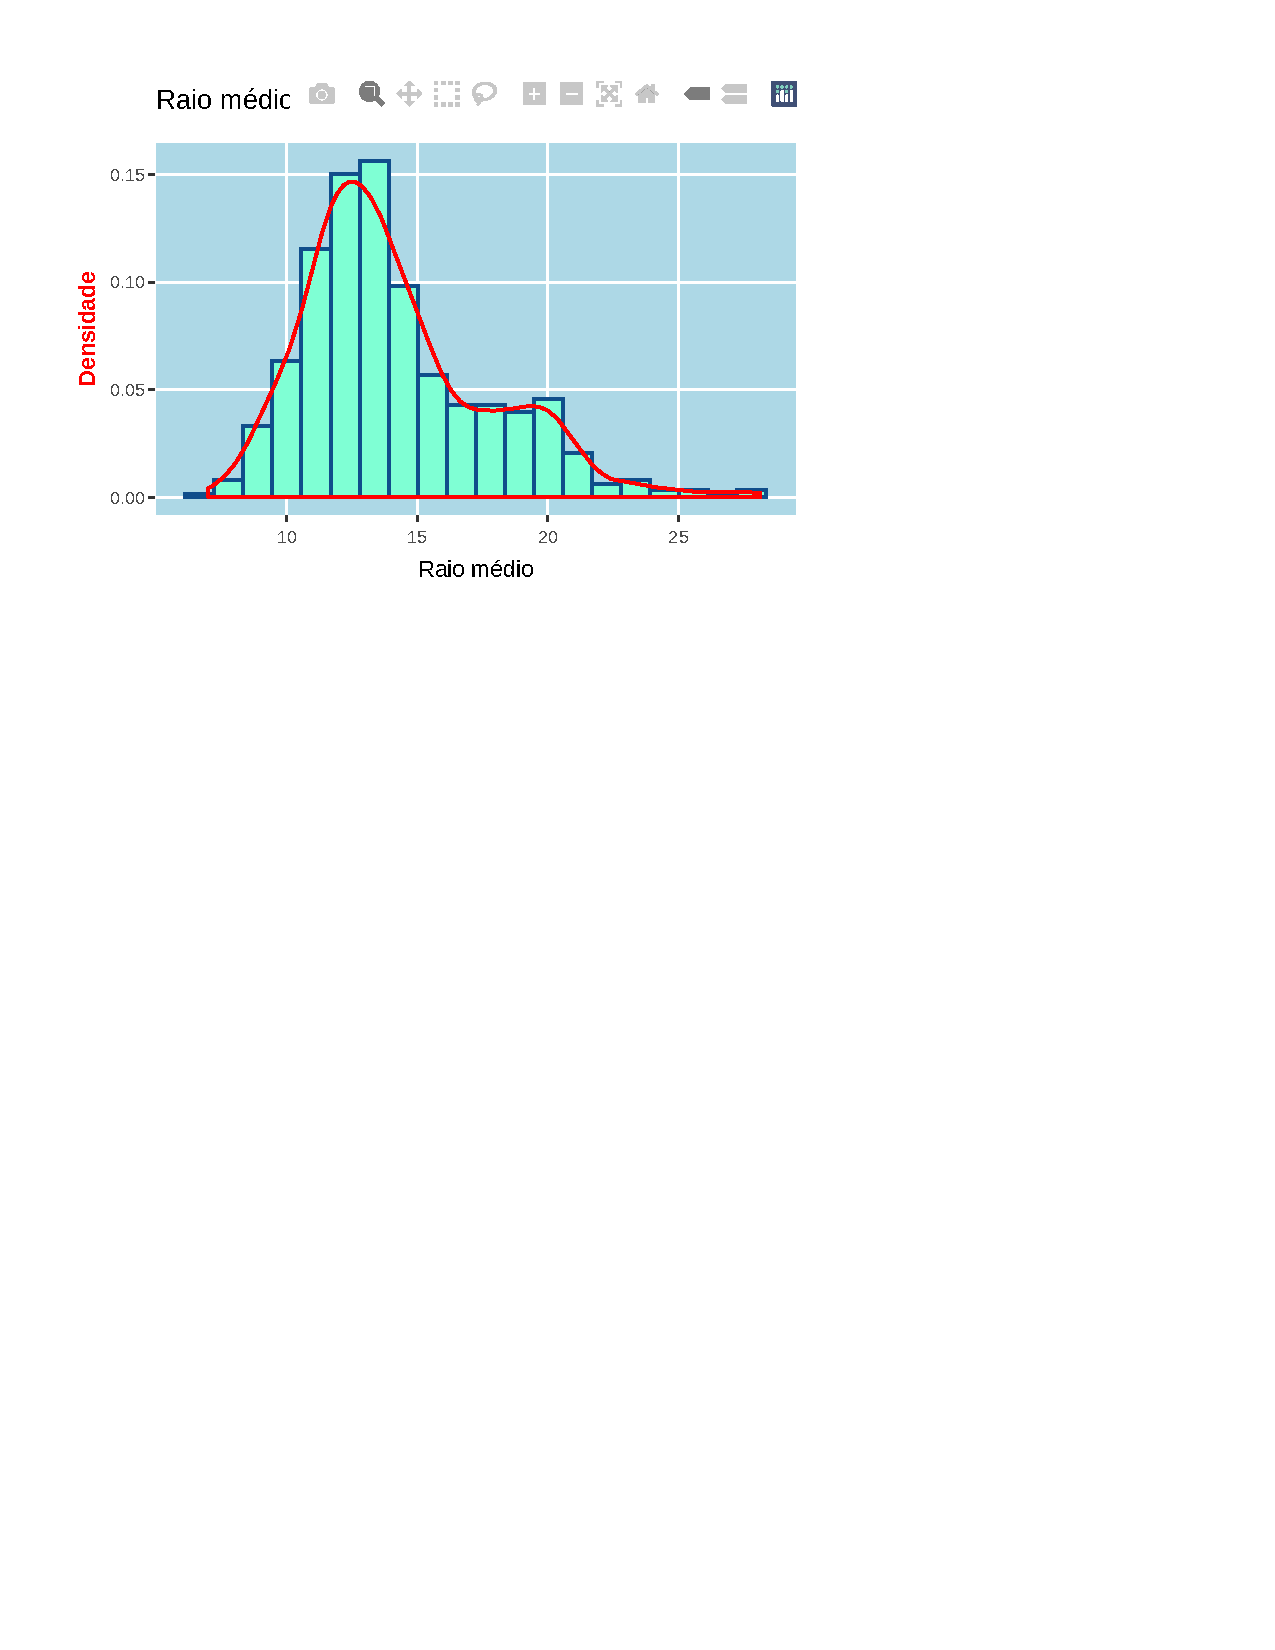
\includegraphics{_main_files/figure-latex/unnamed-chunk-108-1.pdf}

\begin{Shaded}
\begin{Highlighting}[]
\CommentTok{\# Barplot}
\FunctionTok{ggplotly}\NormalTok{(}\FunctionTok{ggplot}\NormalTok{(brca,}
                \FunctionTok{aes}\NormalTok{(Area)) }\SpecialCharTok{+}
           \FunctionTok{geom\_bar}\NormalTok{(}\AttributeTok{stat=}\StringTok{"count"}\NormalTok{, }\FunctionTok{aes}\NormalTok{(}\AttributeTok{fill=}\NormalTok{Area)))}
\end{Highlighting}
\end{Shaded}

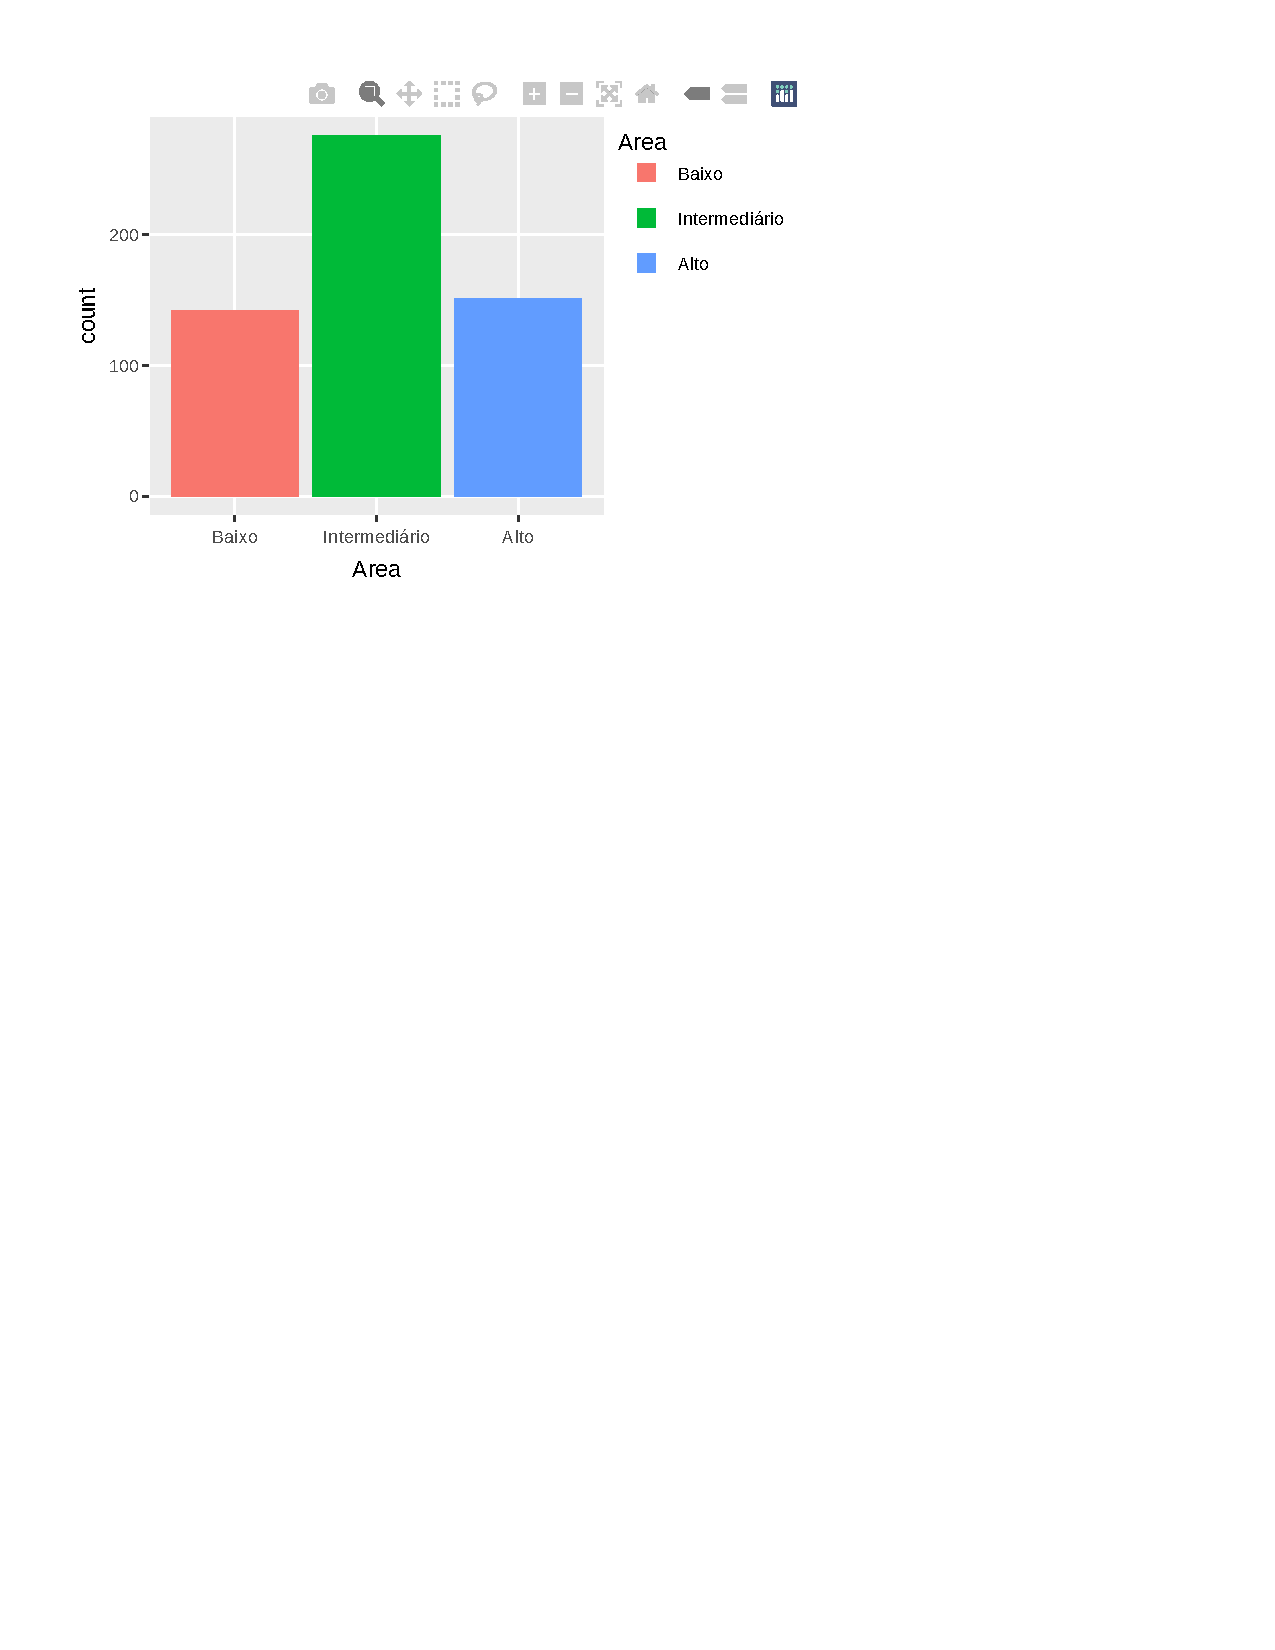
\includegraphics{_main_files/figure-latex/unnamed-chunk-108-2.pdf}

\begin{Shaded}
\begin{Highlighting}[]
\CommentTok{\# Você pode testar com os demais exemplos que criamos na seção anterior}
\CommentTok{\# Crie seu gráfico no ggplot e insira dentro da função ggplotly.}
\CommentTok{\# Perceba que as funções do ggpubr (de comparação estatística)}
\CommentTok{\# ainda não são suportados pelo plotly}

\FunctionTok{ggplotly}\NormalTok{(}\FunctionTok{ggplot}\NormalTok{(mpg, }\FunctionTok{aes}\NormalTok{(}\AttributeTok{x=}\NormalTok{cyl, }\AttributeTok{y=}\NormalTok{hwy, }\AttributeTok{fill=}\FunctionTok{as.factor}\NormalTok{(cyl), }\AttributeTok{group=}\NormalTok{cyl))}\SpecialCharTok{+}
           \FunctionTok{geom\_boxplot}\NormalTok{())}
\end{Highlighting}
\end{Shaded}

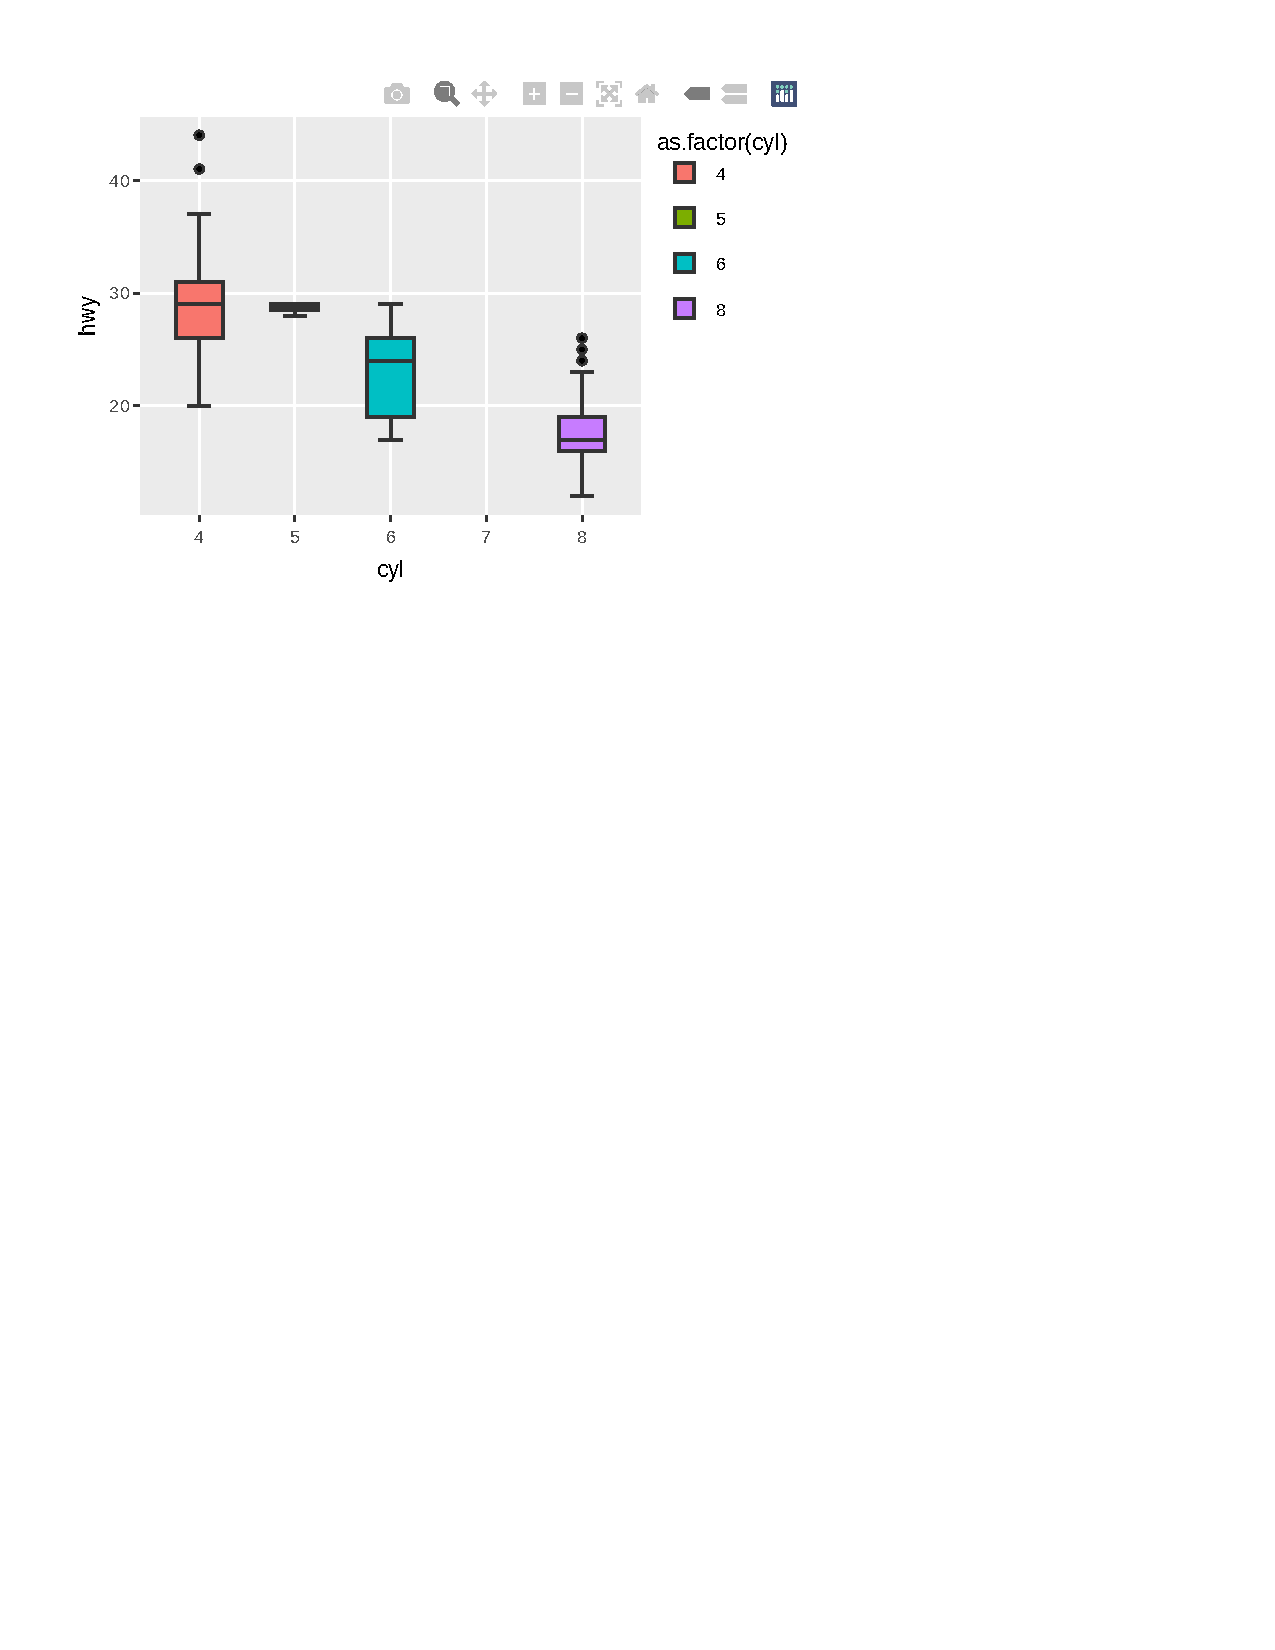
\includegraphics{_main_files/figure-latex/unnamed-chunk-108-3.pdf}

\begin{Shaded}
\begin{Highlighting}[]
\FunctionTok{summary}\NormalTok{(}\FunctionTok{as.factor}\NormalTok{(mpg}\SpecialCharTok{$}\NormalTok{cyl))}
\end{Highlighting}
\end{Shaded}

\begin{verbatim}
##  4  5  6  8 
## 81  4 79 70
\end{verbatim}

\hypertarget{lista-de-exercuxedcios-02}{%
\section{Lista de exercícios 02}\label{lista-de-exercuxedcios-02}}

\begin{enumerate}
\def\labelenumi{\arabic{enumi}.}
\item
  Utilizando o data set mpg: como você plotaria a relação entre as variáveis cty (a milhagem média da cidade) e hwy (a quilometragem média da rodovia)? Como você descreveria essa relação?
\item
  Para adicionar variáveis a um gráfico precisamos mapeá-las em estéticas. Em duas dimensões, podemos usar os eixos x e y. Para adicionar uma terceira (ou quarta, etc) variável precisamos utilizar estéticas tais como forma, cor e tamanho. Utilizando o data set mpg, plote um gráfico de pontos usando a função ggplot, mostrando a relação entre as variáveis displ, hwy e drv. Dica: como se tratam de mais de duas variáveis, use a estética shape para representar drv.
\item
  Continuando a usar o data set mpg, vamos primeiro ver como fica a distribuição dos dados de milhas rodadas na cidade por galões de combustível (cty). Para isso, crie um histograma básico com a variável cty, use o argumento breaks = 10. Os valores se concentram ao redor de qual número?
\item
  Agora vamos investigar como o consumo urbano se comporta dependendo da classe do
  carro. Crie um boxplot onde o eixo x serão as classes dos carros (class) e no eixo y a quantidade de milhas que o carro faz por galão de combustível (cty). Valores mais altos em cty indicam carros que gastam menos combustível. Quais as 2 classes mais econômicas na cidade (maiores valores em cty)? Quais as 2 classes que mais consomem combustível na cidade (menores valores em cty)?
\end{enumerate}

  \bibliography{book.bib,packages.bib}

\end{document}
